\documentclass[a4paper]{article}

%=========================================
% Packages
%=========================================
\usepackage{mathtools}
\usepackage{amsfonts}
\usepackage{amsmath}
\usepackage{amssymb}
\usepackage{amsthm}
\usepackage[a4paper, total={6in, 8in}, margin=1in]{geometry}
\usepackage[utf8]{inputenc}
\usepackage{fancyhdr}
\usepackage[utf8]{inputenc}
\usepackage{graphicx}
\usepackage{physics}
\usepackage[listings]{tcolorbox}
\usepackage{hyperref}
\usepackage{tikz-cd}
\usepackage{adjustbox}
\usepackage{enumitem}
\usepackage[font=small,labelfont=bf]{caption}
\usepackage{subcaption}
\usepackage{wrapfig}
\usepackage{makecell}



\raggedright

\usetikzlibrary{arrows.meta}

\DeclarePairedDelimiter\ceil{\lceil}{\rceil}
\DeclarePairedDelimiter\floor{\lfloor}{\rfloor}

%=========================================
% Fonts
%=========================================
\usepackage{tgpagella}
\usepackage[T1]{fontenc}


%=========================================
% Custom Math Operators
%=========================================
\DeclareMathOperator{\adj}{adj}
\DeclareMathOperator{\im}{im}
\DeclareMathOperator{\nullity}{nullity}
\DeclareMathOperator{\sign}{sign}
\DeclareMathOperator{\dom}{dom}
\DeclareMathOperator{\lcm}{lcm}
\DeclareMathOperator{\ran}{ran}
\DeclareMathOperator{\ext}{Ext}
\DeclareMathOperator{\dist}{dist}
\DeclareMathOperator{\diam}{diam}
\DeclareMathOperator{\aut}{Aut}
\DeclareMathOperator{\inn}{Inn}
\DeclareMathOperator{\syl}{Syl}
\DeclareMathOperator{\edo}{End}
\DeclareMathOperator{\cov}{Cov}
\DeclareMathOperator{\vari}{Var}
\DeclareMathOperator{\cha}{char}
\DeclareMathOperator{\Span}{span}
\DeclareMathOperator{\ord}{ord}
\DeclareMathOperator{\res}{res}
\DeclareMathOperator{\Hom}{Hom}
\DeclareMathOperator{\Mor}{Mor}
\DeclareMathOperator{\coker}{coker}
\DeclareMathOperator{\Obj}{Obj}
\DeclareMathOperator{\id}{id}
\DeclareMathOperator{\GL}{GL}
\DeclareMathOperator*{\colim}{colim}

%=========================================
% Custom Commands (Shortcuts)
%=========================================
\newcommand{\CP}{\mathbb{CP}}
\newcommand{\GG}{\mathbb{G}}
\newcommand{\F}{\mathbb{F}}
\newcommand{\N}{\mathbb{N}}
\newcommand{\Q}{\mathbb{Q}}
\newcommand{\R}{\mathbb{R}}
\newcommand{\C}{\mathbb{C}}
\newcommand{\E}{\mathbb{E}}
\newcommand{\Prj}{\mathbb{P}}
\newcommand{\RP}{\mathbb{RP}}
\newcommand{\T}{\mathbb{T}}
\newcommand{\Z}{\mathbb{Z}}
\newcommand{\A}{\mathbb{A}}
\renewcommand{\H}{\mathbb{H}}
\newcommand{\K}{\mathbb{K}}

\newcommand{\mA}{\mathcal{A}}
\newcommand{\mB}{\mathcal{B}}
\newcommand{\mC}{\mathcal{C}}
\newcommand{\mD}{\mathcal{D}}
\newcommand{\mE}{\mathcal{E}}
\newcommand{\mF}{\mathcal{F}}
\newcommand{\mG}{\mathcal{G}}
\newcommand{\mH}{\mathcal{H}}
\newcommand{\mI}{\mathcal{I}}
\newcommand{\mJ}{\mathcal{J}}
\newcommand{\mK}{\mathcal{K}}
\newcommand{\mL}{\mathcal{L}}
\newcommand{\mM}{\mathcal{M}}
\newcommand{\mO}{\mathcal{O}}
\newcommand{\mP}{\mathcal{P}}
\newcommand{\mS}{\mathcal{S}}
\newcommand{\mT}{\mathcal{T}}
\newcommand{\mV}{\mathcal{V}}
\newcommand{\mW}{\mathcal{W}}

%=========================================
% Colours!!!
%=========================================
\definecolor{LightBlue}{HTML}{2D64A6}
\definecolor{ForestGreen}{HTML}{4BA150}
\definecolor{DarkBlue}{HTML}{000080}
\definecolor{LightPurple}{HTML}{cc99ff}
\definecolor{LightOrange}{HTML}{ffc34d}
\definecolor{Buff}{HTML}{DDAE7E}
\definecolor{Sunset}{HTML}{F2C57C}
\definecolor{Wenge}{HTML}{584B53}
\definecolor{Coolgray}{HTML}{9098CB}
\definecolor{Lavender}{HTML}{D6E3F8}
\definecolor{Glaucous}{HTML}{828BC4}
\definecolor{Mauve}{HTML}{C7A8F0}
\definecolor{Darkred}{HTML}{880808}
\definecolor{Beaver}{HTML}{9A8873}
\definecolor{UltraViolet}{HTML}{52489C}



%=========================================
% Theorem Environment
%=========================================
\tcbuselibrary{listings, theorems, breakable, skins}

\newtcbtheorem[number within = subsection]{thm}{Theorem}%
{	colback=Buff!3, 
	colframe=Buff, 
	fonttitle=\bfseries, 
	breakable, 
	enhanced jigsaw, 
	halign=left
}{thm}

\newtcbtheorem[number within=subsection, use counter from=thm]{defn}{Definition}%
{  colback=cyan!1,
    colframe=cyan!50!black,
	fonttitle=\bfseries, breakable, 
	enhanced jigsaw, 
	halign=left
}{defn}

\newtcbtheorem[number within=subsection, use counter from=thm]{axm}{Axiom}%
{	colback=red!5, 
	colframe=Darkred, 
	fonttitle=\bfseries, 
	breakable, 
	enhanced jigsaw, 
	halign=left
}{axm}

\newtcbtheorem[number within=subsection, use counter from=thm]{prp}{Proposition}%
{	colback=LightBlue!3, 
	colframe=Glaucous, 
	fonttitle=\bfseries, 
	breakable, 
	enhanced jigsaw, 
	halign=left
}{prp}

\newtcbtheorem[number within=subsection, use counter from=thm]{lmm}{Lemma}%
{	colback=LightBlue!3, 
	colframe=LightBlue!60, 
	fonttitle=\bfseries, 
	breakable, 
	enhanced jigsaw, 
	halign=left
}{lmm}

\newtcbtheorem[number within=subsection, use counter from=thm]{crl}{Corollary}%
{	colback=LightBlue!3, 
	colframe=LightBlue!60, 
	fonttitle=\bfseries, 
	breakable, 
	enhanced jigsaw, 
	halign=left
}{crl}

\newtcbtheorem[number within=subsection, use counter from=thm]{eg}{Example}%
{	colback=Beaver!5, 
	colframe=Beaver, 
	fonttitle=\bfseries, 
	breakable, 
	enhanced jigsaw, 
	halign=left
}{eg}

\newtcbtheorem[number within=subsection, use counter from=thm]{ex}{Exercise}%
{	colback=Beaver!5, 
	colframe=Beaver, 
	fonttitle=\bfseries, 
	breakable, 
	enhanced jigsaw, 
	halign=left
}{ex}

\newtcbtheorem[number within=subsection, use counter from=thm]{alg}{Algorithm}%
{	colback=UltraViolet!5, 
	colframe=UltraViolet, 
	fonttitle=\bfseries, 
	breakable, 
	enhanced jigsaw, 
	halign=left
}{alg}




%=========================================
% Hyperlinks
%=========================================
\hypersetup{
    colorlinks=true, %set true if you want colored links
    linktoc=all,     %set to all if you want both sections and subsections linked
    linkcolor=DarkBlue,  %choose some color if you want links to stand out
}


\pagestyle{fancy}
\fancyhf{}
\rhead{Labix}
\lhead{Algebraic Topology 2}
\rfoot{\thepage}

\title{Algebraic Topology 2}

\author{Labix}

\date{\today}
\begin{document}
\maketitle
\begin{abstract}
Algebraic Topology 2 concerns two new algebraic invariants for topological spaces. The homology groups of a space is more powerful than the fundamental group in identifying homeomorphic spaces. However it is also harder to compute, and requires more algebraic background to power the engine. The cohomology ring on the other hand lies in between the homotopy groups and the homology groups. It has a richer structure which enables it to distinguish more spaces, and it is easier to calculate than homology in some cases. \\~\\

References: 
\begin{itemize}
\item Notes on Algebraic Topology by Oscar Randal-Williams
\item Notes on MA3H6 Algebraic Topology 2 by Martin Gallauer
\item Algebraic Topology by Allen Hatcher
\end{itemize}
\end{abstract}
\pagebreak
\tableofcontents

\pagebreak
\section{The Categorical Viewpoint}
Recall that the category of topological spaces $\bold{Top}$ is complete and cocomplete. This means that all kinds of limits and colimits exists in $\bold{Top}$. We have already seen the product space and disjoint union with their universal property as a limit / colimit. There are also more constructs that can be recognized / defined in terms of the universal property. 

\subsection{Different Categories of Spaces}
\begin{defn}{The Category of Pointed Topological Spaces}{} Define the category of pointed topological spaces $\bold{Top}_\ast$ to consist of the following data. 
\begin{itemize}
\item The objects are a pair $(X,x_0)$ where $X$ is a topological space and $x_0\in X$ is a chosen base point. 
\item For $(X,x_0)$ and $(Y,y_0)$ two pointed spaces, the morphisms $$\Hom_{\bold{Top}_\ast}((X,x_0),(Y,y_0))=\{f:X\to Y\;|\;f\text{ is continuous and }f(x_0)=y_0\}$$ are the continuous maps from $X$ to $Y$ such that base points are preserved. 
\item Composition is defined as the composition of functions such that base point is preserved. 
\end{itemize}
\end{defn}

\begin{prp}{}{} Let $(X,x_0)$ and $(Y,y_0)$ be pointed spaces. Then the product and coproduct of the two spaces in $\bold{Top}_\ast$ are $$(X\times Y,(x_0,y_0))\;\;\;\;\text{ and }\;\;\;\;(X\vee Y,x_0=y_0)$$ respectively. 
\end{prp}

\begin{defn}{The Category of CW Complexes}{} Define the category of CW complexes $\bold{CW}$ to consist of the following data. 
\begin{itemize}
\item The objects are CW complexes. 
\item For $X$ and $Y$ two CW complexes, the morphisms $$\Hom_{\bold{CW}}(X,Y)=\{f:X\to Y\;|\;f\text{ is continuous}\}$$ are the continuous maps from $X$ to $Y$. 
\item Composition is defined as the composition of functions. 
\end{itemize}
Define similarly the category $\bold{CW}_\ast$ of pointed topological spaces. 
\end{defn}

\begin{defn}{The Category of Pairs of Spaces}{} Define the category of pairs of topological spaces $\bold{Top}^2$ to consist of the following data. 
\begin{itemize}
\item The objects are a pair $(X,A)$ where $X$ is a topological space $A\subseteq X$ is a subspace of $X$. 
\item For $(X,A)$ and $(Y,B)$ two pointed spaces, the morphisms $$\Hom_{\bold{Top}^2}((X,A),(Y,B))=\{f:X\to Y\;|\;f\text{ is continuous and }f(A)\subseteq B\}$$ are the continuous maps from $X$ to $Y$ such that subspaces are mapped to subspaces. 
\item Composition is defined as the composition of functions such that subspaces are mapped to subspaces. 
\end{itemize}
Define similarly the category $\bold{CW}^2$ of pairs of CW complexes. 
\end{defn}

\begin{defn}{Homotopy Category of Spaces}{} Define the homotopy category of topological spaces $\bold{hTop}$ to consist of the following data. 
\begin{itemize}
\item The objects are topological spaces. 
\item For $X$ and $Y$ two spaces, the morphisms $$\Hom_{\bold{CW}}(X,Y)=\{f:X\to Y\;|\;f\text{ is continuous}\}/\sim$$ are the homotopy classes of continuous maps from $X$ to $Y$. 
\item Composition is defined as the composition of functions. 
\end{itemize}
Define similar the homotopy category $\bold{hTop}_\ast$ of pointed topological spaces and pointed homotopy classes of maps. 
\end{defn}

\subsection{Categorical Constructs in the Category of Spaces}
We have seen pushouts and pullbacks in Category Theory 1. Let us first recall them. 

\begin{defn}{Adjunction Spaces}{} Let $X,Y$ be spaces and $A\subseteq X$ a subspace. Let $f:A\to Y$ be a map. Define the adjunction space of $X$ and $Y$ to be  the space $$X\amalg_fY=\frac{X\amalg Y}{a\sim f(a)}$$ together with the quotient topology. 
\end{defn}

The prototypical example of adjunction spaces come from CW complexes. It is easy to notice that the data of obtaining the $(n+1)$-skeleton inductively is the same content of a pushout diagram: \\~\\
\adjustbox{scale=1.0,center}{\begin{tikzcd}
	{S_\alpha^{n-1}} & {X^n} \\
	{D_\alpha^n} & {X^{n+1}}
	\arrow["{\varphi_\alpha}", from=1-1, to=1-2]
	\arrow[hook, from=1-1, to=2-1]
	\arrow[from=1-2, to=2-2]
	\arrow["{\Phi_\alpha}"', from=2-1, to=2-2]
\end{tikzcd}}\\~\\
Indeed $\Phi_\alpha$ is determined by $\varphi_\alpha$ as a property of the pushout. Collectively, we identify the attaching of all $n$-cells as the following pushout: \\~\\
\adjustbox{scale=1.0,center}{\begin{tikzcd}
	{\coprod_{\alpha\in I_n}S_\alpha^{n-1}} && {X^n} \\
	\\
	{\coprod_{\alpha\in I_n}D_\alpha^n} && {X^{n+1}}
	\arrow["{\coprod_{\alpha\in I_n}\varphi_\alpha}", from=1-1, to=1-3]
	\arrow[hook, from=1-1, to=3-1]
	\arrow[from=1-3, to=3-3]
	\arrow["{\coprod_{\alpha\in I_n}\Phi_\alpha}"', from=3-1, to=3-3]
\end{tikzcd}}\\~\\

The final CW complex $X$ is then obtained by the union with the weak topology. But this is just the explicit description of the colimit of the $n$-skeletons. 

\begin{prp}{}{} Let $X,Y$ be spaces and $A\subseteq X$ a subspace of $X$. Let $f:A\to Y$ be a map. Then the adjunction space $X\amalg_f Y$ is a pushout of $f$ and $i:A\to X$ in $\bold{Top}$. 
\end{prp}

\begin{prp}{}{} Let $X,Y$ be spaces with chosen base point $x_0$ and $y_0$ respectively. Then the wedge product $$X\vee Y=X\amalg_fY$$ is an adjunction space with $Z=\{x_0\}$ and map $f:Z\to Y$ defined by $f(x_0)=y_0$. 
\end{prp}

\pagebreak

\section{Algebra of Chain Complexes}
Homological algebra is the backbone for algebraic topology. In this chapter we will first develop all related notions of chain complexes and exact sequences before diving into the topology side of things. 

\subsection{Chain Complexes}
We begin with a very important notion in homological algebra. A chain complex records a sequence of abelian groups together with group homomorphisms that connect them up. All of homology and cohomology starts with establish a chain complex out of a topological space. 

\begin{defn}{Chain Complex}{1.1.1} Let $R$ be a ring. A chain complex $(C_\bullet,\partial_\bullet)$ is a family of $R$-modules $C_n$ for $n\in\Z$ and $R$-module homomorphisms $\partial_n:C_n\to C_{n-1}$ such that $\partial_n\circ\partial_{n+1}=0$ for all $n$. Explicitly, we have a diagram as follows: \\
\adjustbox{scale=1.0,center}{\begin{tikzcd}
	\cdots & {C_{n+1}} & {C_n} & {C_{n-1}} & \cdots
	\arrow[from=1-1, to=1-2]
	\arrow["{\partial_{n+1}}", from=1-2, to=1-3]
	\arrow["{\partial_n}", from=1-3, to=1-4]
	\arrow[from=1-4, to=1-5]
\end{tikzcd}}\\~\\
for which we require that $$\im(\partial_{n+1})\subseteq\ker(\partial_n)$$ for each $n$. 
\end{defn}

We can relate short exact sequences with chain complexes. In particular, one can always extract short exact sequences from chain complexes. 

\begin{lmm}{}{1.1.2} Let $(C_\bullet,\partial_\bullet)$ be a chain complex over $\Z$. Then for any $n$, the sequence \\~\\
\adjustbox{scale=1.0,center}{\begin{tikzcd}
	0 & {Z_n(C_\bullet)} & {C_n} & {B_{n-1}(C_\bullet)} & 0
	\arrow[from=1-1, to=1-2]
	\arrow["\iota", from=1-2, to=1-3]
	\arrow["{\partial_n}", from=1-3, to=1-4]
	\arrow[from=1-4, to=1-5]
\end{tikzcd}}\\~\\
is a short exact sequence. Moreover, if the terms of the chain complex consist of free abelian groups, then the sequence is split exact. \tcbline
\begin{proof}
The inclusion map is injective. $\partial_n$ is also surjective on its image. Finally, $\ker(\partial_n)$ is by definition $Z_n(C_\bullet)\cong\im(\iota)$. Now since subgroups of a free abelian group are free, we conclude that $B_{n-1}\leq C_n$ is free. Recall that if the third term of a short exact sequence is free, the sequence is split. Hence we conclude. 
\end{proof}
\end{lmm}

It is routine to also define maps between chain complexes. Indeed in Groups and Rings we introduced groups and group homomorphisms. In Topology we defined topological spaces and continuous maps. For chain complexes we have the notion of chain maps. 

\begin{defn}{Chain Map}{1.1.3} Let $R$ be a ring. Let $(C_\bullet,\partial_\bullet)$ and $(D_\bullet,\partial_\bullet')$ be two chain complexes over $R$. A chain map $f_\bullet:C_\bullet\to D_\bullet$ is a family of $R$-module homomorphisms $$f_n:C_n\to D_n$$ such that $\partial_n'\circ f_n=f_{n-1}\circ\partial_n$ for all $n$. Explicitly, we have the following commutative diagram: \\~\\
\adjustbox{scale=1.0,center}{\begin{tikzcd}
	\cdots & {C_{n+1}} & {C_n} & {C_{n-1}} & \cdots \\
	\cdots & {D_{n+1}} & {D_n} & {D_{n-1}} & \cdots
	\arrow[from=1-1, to=1-2]
	\arrow["{\partial_{n+1}}", from=1-2, to=1-3]
	\arrow["{f_{n+1}}"', from=1-2, to=2-2]
	\arrow["{\partial_n}", from=1-3, to=1-4]
	\arrow["{f_n}"', from=1-3, to=2-3]
	\arrow[from=1-4, to=1-5]
	\arrow["{f_{n-1}}", from=1-4, to=2-4]
	\arrow[from=2-1, to=2-2]
	\arrow["{\partial_{n+1}'}"', from=2-2, to=2-3]
	\arrow["{\partial_n'}"', from=2-3, to=2-4]
	\arrow[from=2-4, to=2-5]
\end{tikzcd}}
\end{defn}

It is customary to drop the $n\in\N$ in the notation as it is usually implicit. So for example the condition for chain map becomes $\partial'\circ f=f\circ\partial$. 

\begin{lmm}{}{1.1.4} Let $R$ be a ring. Let $C_\bullet,D_\bullet,E_\bullet$ be chain complexes over $R$. Let $f:C_\bullet\to D_\bullet$ and $g:D_\bullet\to E_\bullet$ be chain maps. Then the term-wise composition of $f$ and $g$ also gives a chain map $g\circ f:C_\bullet\to D_\bullet$. 
\end{lmm}

\begin{defn}{The Category of Chain Complexes}{1.1.5} Let $R$ be a ring. Define the category of chain complexes $$\bold{Ch}(R)$$ over $R$ to consist of the following data. 
\begin{itemize}
\item The objects are the chain complexes over $R$
\item The morphisms are the chain maps
\item Composition is given by the term-wise composition of maps on all levels. 
\end{itemize}
\end{defn}

\begin{defn}{Homology Group}{1.1.6} Let $R$ be a ring. Let $(C_\bullet,\partial_\bullet)$ be a chain complex over $R$. 
\begin{itemize}
\item Define the the $R$-submodule of $n$-cycles of the chain complex to be $$Z_n(C_\bullet)=\ker(\partial_n)$$
\item Define the $R$-submodule of $n$-boundaries of the chain complex to be $$B_n(C_\bullet)=\im(\partial_{n+1})$$
\item Define the $n$th homology of the chain complex to be $$H_n(C_\bullet)=\frac{Z_n(C_\bullet)}{B_n(C_\bullet)}=\frac{\ker(\partial_n)}{\im(\partial_{n+1})}$$
\end{itemize}
\end{defn}

\begin{defn}{Induced Homomorphisms}{1.1.7} Let $R$ be a ring. Let $C_\bullet$ and $D_\bullet$ be chain complexes over $R$. Let $f:C_\bullet\to D_\bullet$ be a chain map. Define the induced map on homology $$f_\ast:H_n(C_\bullet)\to H_n(D_\bullet)$$ by the formula $f_\ast([z])=[f(z)]$. 
\end{defn}

\begin{lmm}{}{1.1.8} Let $R$ be a ring. Let $C_\bullet$ and $C_\bullet'$ be chain complexes over $R$. Let $f:C_\bullet\to C_\bullet'$ be a chain map. Then the induced map on homology $$f_\ast:H_n(C_\bullet)\to H_n(C_\bullet')$$ is a well defined $R$-module homomorphism. \tcbline
\begin{proof}
For every map $f_n:C_n\to C_n'$, we can restrict the domain to cycles so that we obtain a map $f_n:Z_n(C_\bullet)\to C_n'$. Using the relation given between the boundary operator and the family of maps, we check that this map descends to a map in homology. \\~\\

Firstly, $f_n(Z_n(C_\bullet))\subseteq Z_n(C_\bullet')$. Indeed let $x\in Z_n(C_\bullet)$. Then we have that $$\partial_n'(f_n(x))=f_{n-1}(\partial_n(x))=f_{n-1}(0)=0$$ which means that $f_n(x)$ lies in the kernel of $\partial_n'$. Now we have a map $f_n:Z_n(C_\bullet)\to Z_n(C_\bullet')$. At the same time, $f_n$ also restricts to a map $f_n:B_n(C_\bullet)\to B_n(C_\bullet')$. Indeed if $b\in B_n(C_\bullet)$, then there exists some $c\in C_{n+1}$ such that $\partial_{n+1}(c)=b$. Applying $f_n$ on both sides give 
\begin{align*}
f_n(\partial_{n+1}(c))&=f_n(b)\\
\partial_{n+1}'(f_{n+1}(c))&=f_n(b)
\end{align*}
This means that $f_n(b)$ is the boundary of the element $f_{n+1}(c)\in C_{n+1}$, and so $f_n$ restricts to a map of boundaries. Now $f_n:H_n(C_\bullet)\to H_n(C_\bullet')$ is well defined. Indeed if $b_1,b_2\in B_n(C_\bullet)$ lie in the same coset, then $b_1B_n(C_\bullet)=b_2(C_\bullet)$ so that $b_1-b_2\in B_(C_\bullet)$. Then $f_n(b_1-b_2)\in B_n(C_\bullet')$ so that $f_n(b_1)$ and $f_n(b_2)$ lie in the same coset. Thus $f_n$ is well defined. 
\end{proof}
\end{lmm}

We then have functoriality of the induced map. 

\begin{prp}{}{1.1.9} Let $R$ be a ring. Let $C_\bullet,D_\bullet,E_\bullet$ be chain complexes over $R$. Let $f:C_\bullet\to D_\bullet$ and $g:D_\bullet\to E_\bullet$ be chain maps. Then the induced map on the homology groups satisfy the properties: 
\begin{itemize}
\item $g_\ast\circ f_\ast=(g\circ f)_\ast$
\item $\text{id}_\ast=\text{id}_{H_n}$
\end{itemize} \tcbline
\begin{proof}
Firstly, we have that $$\partial\circ g_n\circ f_n=g_{n-1}\circ\partial\circ f_n=g_{n-1}\circ f_{n-1}\circ\partial$$ so that $g\circ f$ is indeed a chain map. \\~\\

We have that $g_\ast(f_\ast([z]))=g_\ast([f(z)])=[g(f(z))]=(g_\ast\circ f_\ast)([z])$. Also, we have that $$\text{id}_\ast([z])=[\text{id}(z)]=[z]=\text{id}_{H^n}([z])$$ and so we conclude. 
\end{proof}
\end{prp}

\begin{defn}{The Homology Functor}{1.1.10} Let $R$ be a ring. Define the homology functors $$H_n(-):\bold{Ch}(R)\to\bold{Ab}$$ for each $n$ as follows. 
\begin{itemize}
\item For each chain complex $C_\bullet$ over $R$, $H_n(C_\bullet)$ is the $n$th homology group of $C_\bullet$. 
\item For each chain map $f:C_\bullet\to C_\bullet'$, $$H_n(f):H_n(C_\bullet)\to H_n(C_\bullet')$$ is the induced map on homology. 
\end{itemize}
\end{defn}

\subsection{Chain Homotopies}
In algebraic topology 1, we defined the notion of homotopies between two maps. In general, algebraic topologists are not only interested in maps between two objects such as groups or vector spaces, we are also interested in the maps between the maps. Therefore homotopies play such a crucial role in Algebraic Topology 1. In order to produce results similar to homotopy invariance of the fundamental groups, we will need the notion of homotopies between chain maps. \\

One can think of the chain complexes as our objects, chain maps as morphisms between chain complexes and morphisms between chain maps as chain homotopies. This is precisely the notion of the category of chain complexes. 

\begin{defn}{Chain Homotopy}{1.2.1} Let $R$ be a ring. Let $C_\bullet,D_\bullet$ be chain complexes over $R$. Let $f:C_\bullet\to D_\bullet$ and $g:C_\bullet\to D_\bullet$ be chain maps. Then a chain homotopy from $f$ to $g$ is a collection of morphisms $$\eta_n:C_n\to C_{n+1}'\;\;\;\;\text{ such that }\;\;\;\;g_n-f_n=\partial_{n+1}'\eta_n+\eta_{n-1}\partial_n$$ for all $n\in\Z$. Explicitly, the following diagram is commutative: \\~\\
\adjustbox{scale=1.2,center}{\begin{tikzcd}
	\cdots & {C_{n+1}} & {C_n} & {C_{n-1}} & \cdots \\
	\cdots & {D_{n+1}} & {D_n} & {D_{n-1}} & \cdots
	\arrow[from=1-1, to=1-2]
	\arrow["{\partial_{n+1}}", from=1-2, to=1-3]
	\arrow[from=1-2, to=2-1]
	\arrow["{g-f}"', from=1-2, to=2-2]
	\arrow["{\partial_n}", from=1-3, to=1-4]
	\arrow["{\eta_n}"{description}, from=1-3, to=2-2]
	\arrow["{g-f}"{description}, from=1-3, to=2-3]
	\arrow[from=1-4, to=1-5]
	\arrow["{\eta_{n-1}}"{description}, from=1-4, to=2-3]
	\arrow["{g-f}", from=1-4, to=2-4]
	\arrow[from=1-5, to=2-4]
	\arrow[from=2-1, to=2-2]
	\arrow["{\partial_{n+1}'}"', from=2-2, to=2-3]
	\arrow["{\partial_n'}"', from=2-3, to=2-4]
	\arrow[from=2-4, to=2-5]
\end{tikzcd}}\\~\\
In this case, $f$ and $g$ are said to be chain homotopic and we write $f\simeq g$. 
\end{defn}

\begin{lmm}{}{1.2.2} Let $R$ be a ring. Let $C_\bullet,D_\bullet$ be chain complexes over $R$. Then the relation $\simeq$ on the chain maps from $C_\bullet$ to $D_\bullet$ is an equivalence relation. \tcbline
\begin{proof}
Let $f_\bullet,g_\bullet,h_\bullet:C_\bullet\to D_\bullet$ be chain maps. Then it is clear that $f_\bullet\simeq f_\bullet$ by the $0$ map. Indeed we have that $\partial 0+0\partial=0=f-f$. Thus $\simeq$ is reflexive. if $f_\bullet$ and $g_\bullet$ are chain homotopic by $\eta$, then we have the identity $$\partial\eta+\eta\partial=g-f$$ But then we have 
\begin{align*}
f-g&=-\partial\eta-\eta\partial\\
&=\partial(-\eta)+(-\eta)\partial
\end{align*}
which means that $-\eta$ gives a chain homotopy from $g$ to $f$. \\~\\

Now if $g_\bullet$ and $h_\bullet$ are chain homotopic by $\nu$, then we have that 
\begin{align*}
h_\bullet-f_\bullet&=h_\bullet-g_\bullet+g_\bullet-f_\bullet\\
&=\partial\nu+\nu\partial+\partial\eta+\eta\partial\\
&=\partial(\nu+\eta)+(\nu+\eta)\partial
\end{align*}
so that $\nu+\eta$ defines a chain homotopy from $f$ to $h$. 
\end{proof}
\end{lmm}

One consequence of chain homotopies is the following. 

\begin{lmm}{}{1.2.3} Let $R$ be a ring. Let $C_\bullet,D_\bullet$ be chain complexes over $R$. Let $f:C_\bullet\to D_\bullet$ and $g:C_\bullet\to D_\bullet$ be chain maps. If $f$ and $g$ are chain homotopic, then $f$ and $g$ induce the same map $$f_n=g_n:H_n(X)\to H_n(Y)$$ in homology. \tcbline
\begin{proof}
Let $c\in\ker(\partial_n)$ be an $n$-cycle. Using the equation for chain homotopy, we have that 
\begin{align*}
b(c)-a(c)&=\partial_{n+1}'(\eta_n(c))+\eta_{n-1}(\partial(c))\\
&=\partial_{n+1}'(\eta(c))
\end{align*}
 is a boundary in $\im(\partial_{n+1}')\subseteq C_n'$. Thus $b_n(c)$ and $a_n(c)$ are of the same coset in $H_n(X)$. 
\end{proof}
\end{lmm}

Chain homotopies are also well defined in compositions. 

\begin{prp}{}{1.2.4} Let $R$ be a ring. Let $C_\bullet,D_\bullet$ be chain complexes over $R$. Let $f_1,g_1:C_\bullet\to D_\bullet$ and $f_2,g_2:C_\bullet\to D_\bullet$ be chain maps. If $f_1\simeq g_1$ and $f_2\simeq g_2$, then $f_2\circ f_1\simeq g_2\circ g_1$. \tcbline
\begin{proof}
The chain homotopies between $f_1$ and $g_1$ imposes the identity $$\partial\eta+\eta\partial=g_1-f_1$$ for $\eta:C_\bullet\to D_\bullet$ the given chain homotopy. Similarly, for $\nu:D_\bullet\to E_\bullet$ we have the identity $$\partial\nu+\nu\partial=g_2-f_2$$ Then we have that 
\begin{align*}
g_2\circ g_1-f_2\circ f-1&=g_2\circ g_1-g_2\circ f_1+g_2\circ f_1-f_2\circ f_1\\
&=g_2(g_1-f_1)+(g_2-f_2)\circ f_1\\
&=g_2(\partial\eta+\eta\partial)+(\partial\nu+\nu\partial)\circ f_1\\
&=\partial g_2\eta+g_2\eta\partial+\partial\nu f_1+\nu f_1\partial\\
&=\partial(g_2\eta+\nu f_1)+(g_2\eta+\nu f_1)\partial
\end{align*}
Thus $g_2\eta+\nu f_1:C_n\to E_{n+1}$ would be a valid chain homotopy from $g_2\circ g_1$ to $f_2\circ f_1$. 
\end{proof}
\end{prp}

While chain maps induce a map on the homology groups, we will see that chain homotopy equivalences induces isomorphisms on the homology groups, intuitively because they produce an inverse for each map on the level of homology. 

\begin{defn}{Chain Homotopy Equivalence}{1.2.5} Let $R$ be a ring. Let $C_\bullet,D_\bullet$ be chain complexes over $R$. We say that they are chain homotopy equivalence if there exists chain maps $f_\bullet:C_\bullet\to D_\bullet$ and $g_\bullet:D_\bullet\to C_\bullet$ such that there are chain homotopies $$g_\bullet\circ f_\bullet\simeq\text{id}_{C_\bullet}\;\;\;\;\text{ and }\;\;\;\;f_\bullet\circ g_\bullet\simeq\text{id}_{D_\bullet}$$ In this case, we say that $g$ is a chain homotopy inverse of $f$. 
\end{defn}

\begin{lmm}{}{1.2.6} Let $R$ be a ring. Let $C_\bullet,D_\bullet$ be chain complexes over $R$. Suppose that $f:C_\bullet\to D_\bullet$ is a chain map that induces a chain homotopy equivalence between $C_\bullet$ and $D_\bullet$. Then $f$ induces an isomorphism $$H_n(C_\bullet)\cong H_n(D_\bullet)$$ in all degrees $n\in\N$. \tcbline
\begin{proof}
Suppose that $g$ is the chain homotopy inverse of $f$. We know that $g_\bullet\circ f_\bullet\simeq\text{id}_{C_\bullet}$ which means that they induce the same map: $$g_\ast\circ f_\ast=\text{id}_{H_n(C_\bullet)}$$ Similarly the chain homotopies $f_\bullet\circ g_\bullet\simeq\text{id}_{D_\bullet}$ induce the same map $$f_\ast\circ g_\ast:\text{id}_{H_n(D_\bullet)}$$ as the identity. Then these two identities mean that $f_\ast$ is both injective and surjective. 
\end{proof}
\end{lmm}

Similar to homotopies in Algebraic Topology, chain homotopy also defines an equivalence relation on all the chain maps. 

\begin{prp}{}{1.2.7} Chain homotopy equivalence defines an equivalence relation on all chain complexes. \tcbline
\begin{proof}
Clearly any chain complex is chain homotopy equivalent to itself by the identity map. If $C_\bullet$ and $D_\bullet$ are chain homotopy equivalent by the chain maps $a_\bullet:C_\bullet\to D_\bullet$ and $b_\bullet:D_\bullet\to C_\bullet$, then we have the identities $b_\bullet\circ a_\bullet=\text{id}_{C_\bullet}$ and $a_\bullet\circ b_\bullet=\text{id}_{D_\bullet}$. We can then read them in reverse so that $D_\bullet$ and $C_\bullet$ are chain homotopy equivalence by the maps $b_\bullet$ and $a_\bullet$. \\~\\

Suppose further that $D_\bullet$ and $E_\bullet$ are chain homotopy equivalent via the maps $u_\bullet:D_\bullet\to E_\bullet$ and $v_\bullet:E_\bullet\to D_\bullet$. Then the maps $u_\bullet\circ a_\bullet$ and $b_\bullet\circ v_\bullet$ give a chain homotopy equivalence between $C_\bullet$ and $E_\bullet$. Indeed, upon composition, we have that they are chain  homtopic to the identity maps. 
\end{proof}
\end{prp}

Be careful that chain homotopy defines an equivalence relation on all chain maps between two fixed chain complexes, while chain homotopy equivalence defines an equivalence relation on all chain complexes. One is an equivalence relation on the objects and one is on the morphisms. \\~\\

This is reminiscent to that of ordinary homotopies between continuous maps. Namely, homotopies defines an equivalence relation on all continuous maps between two fixed topological spaces, while homotopy equivalence defines an equivalence relation on all topological spaces. 

\subsection{Sequences of Chain Complexes}
One can even define short exact sequences of chain complexes themselves. 

\begin{defn}{Short Exact Sequence of Chain Complexes}{} Let $R$ be a ring. Let the following be a sequence of homomorphisms in $\bold{Ch}({_R\bold{Mod}})$. \\~\\
\adjustbox{scale=1.0,center}{\begin{tikzcd}
	0 & {A_\bullet} & {B_\bullet} & {C_\bullet} & 0
	\arrow[from=1-1, to=1-2]
	\arrow["f", from=1-2, to=1-3]
	\arrow["g", from=1-3, to=1-4]
	\arrow[from=1-4, to=1-5]
\end{tikzcd}}\\~\\
We say that it is short exact if for each $n\in\N$, the following sequence\\~\\
\adjustbox{scale=1.0, center}{\begin{tikzcd}
	0 & {A_n} & {B_n} & {C_n} & 0
	\arrow[from=1-1, to=1-2]
	\arrow["{f_n}", from=1-2, to=1-3]
	\arrow["{g_n}", from=1-3, to=1-4]
	\arrow[from=1-4, to=1-5]
\end{tikzcd}}\\~\\
is short exact. 
\end{defn}

Explicitly, we can see that a short exact sequence of chain complexes can be written in diagrams as: \\~\\
\adjustbox{scale=1.0,center}{\begin{tikzcd}
	& \vdots & \vdots & \vdots \\
	0 & {A_{n+1}} & {B_{n+1}} & {C_{n+1}} & 0 \\
	0 & {A_n} & {B_n} & {C_n} & 0 \\
	0 & {A_{n-1}} & {B_{n-1}} & {C_{n-1}} & 0 \\
	& \vdots & \vdots & \vdots
	\arrow[from=1-2, to=2-2]
	\arrow[from=1-3, to=2-3]
	\arrow[from=1-4, to=2-4]
	\arrow[from=2-1, to=2-2]
	\arrow["{f_{n+1}}", from=2-2, to=2-3]
	\arrow["\partial"', from=2-2, to=3-2]
	\arrow["{g_{n+1}}", from=2-3, to=2-4]
	\arrow["\partial"', from=2-3, to=3-3]
	\arrow[from=2-4, to=2-5]
	\arrow["\partial", from=2-4, to=3-4]
	\arrow[from=3-1, to=3-2]
	\arrow["{f_n}", from=3-2, to=3-3]
	\arrow["\partial"', from=3-2, to=4-2]
	\arrow["{g_n}", from=3-3, to=3-4]
	\arrow["\partial"', from=3-3, to=4-3]
	\arrow[from=3-4, to=3-5]
	\arrow["\partial", from=3-4, to=4-4]
	\arrow[from=4-1, to=4-2]
	\arrow["{f_{n-1}}", from=4-2, to=4-3]
	\arrow[from=4-2, to=5-2]
	\arrow["{g_{n-1}}", from=4-3, to=4-4]
	\arrow[from=4-3, to=5-3]
	\arrow[from=4-4, to=4-5]
	\arrow[from=4-4, to=5-4]
\end{tikzcd}}\\~\\

\begin{thm}{}{} Let $R$ be a ring. Let the following be a short exact sequence of chain complexes in $\bold{Ch}({_R\bold{Mod}})$. \\~\\
\adjustbox{scale=1.0,center}{\begin{tikzcd}
	0 & {A_\bullet} & {B_\bullet} & {C_\bullet} & 0
	\arrow[from=1-1, to=1-2]
	\arrow["f", from=1-2, to=1-3]
	\arrow["g", from=1-3, to=1-4]
	\arrow[from=1-4, to=1-5]
\end{tikzcd}}\\~\\
Then there exists a connecting homomorphism $d:H_n(C_\bullet)\to H_{n-1}(A_\bullet)$ such that the following sequence of homology groups \\~\\
\adjustbox{scale=1.0,center}{\begin{tikzcd}
	\cdots & {H_{n+1}(C_\bullet)} & {H_n(A_\bullet)} & {H_n(B_\bullet)} & {H_n(C_\bullet)} & {H_{n-1}(A_\bullet)} & \cdots
	\arrow[from=1-1, to=1-2]
	\arrow["d", from=1-2, to=1-3]
	\arrow["{(f_n)_\ast}", from=1-3, to=1-4]
	\arrow["{(g_n)_\ast}", from=1-4, to=1-5]
	\arrow["d", from=1-5, to=1-6]
	\arrow[from=1-6, to=1-7]
\end{tikzcd}}\\~\\
is long exact. Explicitly, $d$ is defined as follows. 
\begin{itemize}
\item Let $[c]\in H_n(C_\bullet)$. By surjectivity of $g_n$ there exists $b\in B_n$ such that $g_n(b)=c$. 
\item We have $c\in Z_n(C_\bullet)$. Because $g_{n-1}(\partial_B(b))=\partial_C(g_n(b))=\partial_C(c)=0$, we have that $\partial_B(b)\in\ker(g_{n-1})=\im(f_{n-1})$. So there exists $a\in A_{n-1}$ such that $f_{n-1}(a)=\partial_B(b)$. 
\end{itemize} 
We then define $$d([c])=[a]$$ \tcbline
\begin{proof}
We want to show that this is well defined. We have made two choices in the definition of $d$. 
\begin{itemize}
\item Suppose that $b,b'\in B_n$ are such that $g_n(b)=c=g_n(b')$. Then $b-b'\in\ker(g_n)=\im(f_n)$ means that there exists $a'\in A_n$ such that $f_n(a'')=b-b'$. Using the same argument from the construction of the map $d$, we obtain $a,a'\in A_{n-1}$ such that $f_{n-1}(a)=\partial_B(b)$ and $f_{n-1}(a')=\partial_B(b')$. This means that $f_{n-1}(a-a')=\partial_B(b-b')=\partial_B(f_n(a''))$. By commutativity of the diagram, we have that $$\partial_B(f_n(a''))=f_{n-1}(\partial_A(a''))$$ so that we have $f_{n-1}(a-a')=f_{n-1}(\partial_A(a''))$. Since $f_{n-1}$ is injective, we conclude that $a-a'=\partial_A(a'')$. But this means that $[a]=[a']$. This implies that the choice of $b$ did not matter in the definition of $d$. 
\item Suppose that $a,a'\in A_{n-1}$ such that $f_{n-1}(a)=\partial_B(b)=f_{n-1}(a')$. Then by injectivity of $f_{n-1}$ we conclude that $a=a'$. 
\end{itemize}
We now need to show that $d$ is well defined under equivalence classes. Suppose that $c\in\im(\partial_C)$. This implies that there exists $c'\in C_{n+1}$ such that $\partial_C(c')=c$. By surjectivity of $g_{n+1}$, there exists $b\in B_{n+1}$ such that $g_{n+1}(b)=c'$. By commutativity of the diagram, we have that $$c=\partial_C(g_{n+1}(b))=g_n(\partial_B(b))$$ Following the construction of $d$, we obtain $a\in A_{n-1}$ such that $f_{n-1}(a)=\partial_B(\partial_B(b))=0$. Hence $a=0$. We conclude that $d$ is a well defined function. We next show that $d$ is an $R$-module homomorphism. \\~\\

Suppose that $[c],[c']\in H_n(C_\bullet)$. Following the construction of $d$ we obtain $b,b'\in B_n$ and $a,a'\in A_{n-1}$ such that $$g_n(b)=c\;\;\;\;g_n(b')=c'\;\;\;\;f_{n-1}(a)=\partial_B(b)\;\;\;\;f_{n-1}(a')=\partial_B(b')$$ We notice that $g_n(b+b')=c+c'$ and $f_{n-1}(a+a')=\partial_B(b+b')$ so that $$d([c+c'])=[a+a']=[a]+[a']=d([c])+d([c'])$$ The prove is similar in showing that $d([rc])=rd([c])$

We also need to show that the long sequence is exact. 
\end{proof}
\end{thm}

Notice that the above theorem is essentially an application of the snake lemma. One can conclude immediately by the snake lemma. \\~\\

The following theorem looks horrifying but it is not as terrible as it looks. In essence, we want to show a naturality condition. This means that given a morphism of short exact sequences of chain complexes, we want an induced map that satisfies some commutative square. 

\begin{thm}{}{} Let $R$ be a ring. Let the following be a short exact sequence of chain complexes in $\bold{Ch}({_R\bold{Mod}})$. Let $A_\bullet,B_\bullet,C_\bullet,A_\bullet',B_\bullet',C_\bullet'$ be six chain complexes and let the following \\~\\
\adjustbox{scale=1.0,center}{\begin{tikzcd}
	0 & {A_\bullet} & {B_\bullet} & {C_\bullet} & 0 \\
	0 & {A_\bullet'} & {B_\bullet'} & {C_\bullet'} & 0
	\arrow[from=1-1, to=1-2]
	\arrow["i", from=1-2, to=1-3]
	\arrow["j", from=1-3, to=1-4]
	\arrow[from=1-4, to=1-5]
	\arrow[from=2-1, to=2-2]
	\arrow["{i'}"', from=2-2, to=2-3]
	\arrow["{j'}"', from=2-3, to=2-4]
	\arrow[from=2-4, to=2-5]
\end{tikzcd}}\\~\\
be two short exact sequence of chain complexes. Let the following diagram be a morphism of the two short exact sequence of chain complexes. \\~\\
\adjustbox{scale=0.9,center}{\begin{tikzcd}
	&&& 0 && 0 && 0 \\
	&& 0 && 0 && 0 \\
	& \cdots && {A_{n+1}'} && {A_n'} && {A_{n-1}'} && \cdots \\
	\cdots && {A_{n+1}} && {A_n} && {A_{n-1}} && \cdots \\
	& \cdots && {B_{n+1}'} && {B_n'} && {B_{n-1}'} && \cdots \\
	\cdots && {B_{n+1}} && {B_n} && {B_{n-1}} && \cdots \\
	& \cdots && {C_{n+1}'} && {C_n'} && {C_{n-1}'} && \cdots \\
	\cdots && {C_{n+1}} && {C_n} && {C_{n-1}} && \cdots \\
	&&& 0 && 0 && 0 \\
	&& 0 && 0 && 0
	\arrow[from=1-4, to=3-4]
	\arrow[from=1-6, to=3-6]
	\arrow[from=1-8, to=3-8]
	\arrow[from=3-2, to=3-4]
	\arrow["d"{pos=0.3}, from=3-4, to=3-6]
	\arrow["{i'}"{pos=0.7}, from=3-4, to=5-4]
	\arrow["d"{pos=0.3}, from=3-6, to=3-8]
	\arrow["{i'}"{pos=0.7}, from=3-6, to=5-6]
	\arrow[from=3-8, to=3-10]
	\arrow["{i'}"{pos=0.7}, from=3-8, to=5-8]
	\arrow[from=4-1, to=4-3]
	\arrow["\alpha"{description}, from=4-3, to=3-4]
	\arrow["\alpha"{description}, from=4-5, to=3-6]
	\arrow["\alpha"{description}, from=4-7, to=3-8]
	\arrow[from=5-2, to=5-4]
	\arrow["d"{pos=0.3}, from=5-4, to=5-6]
	\arrow["{j'}"{pos=0.7}, from=5-4, to=7-4]
	\arrow["d"{pos=0.3}, from=5-6, to=5-8]
	\arrow["{j'}"{pos=0.7}, from=5-6, to=7-6]
	\arrow[from=5-8, to=5-10]
	\arrow["{j'}"{pos=0.7}, from=5-8, to=7-8]
	\arrow[from=6-1, to=6-3]
	\arrow["\beta"{description}, from=6-3, to=5-4]
	\arrow["\beta"{description}, from=6-5, to=5-6]
	\arrow["\beta"{description}, from=6-7, to=5-8]
	\arrow[from=7-2, to=7-4]
	\arrow["d"{pos=0.3}, from=7-4, to=7-6]
	\arrow[from=7-4, to=9-4]
	\arrow["d"{pos=0.3}, from=7-6, to=7-8]
	\arrow[from=7-6, to=9-6]
	\arrow[from=7-8, to=7-10]
	\arrow[from=7-8, to=9-8]
	\arrow[from=8-1, to=8-3]
	\arrow["\gamma"{description}, from=8-3, to=7-4]
	\arrow[from=8-3, to=10-3]
	\arrow["\gamma"{description}, from=8-5, to=7-6]
	\arrow[from=8-5, to=10-5]
	\arrow["\gamma"{description}, from=8-7, to=7-8]
	\arrow[from=8-7, to=10-7]
	\arrow[from=2-3, to=4-3, crossing over]
	\arrow[from=2-5, to=4-5, crossing over]
	\arrow[from=2-7, to=4-7, crossing over]
	\arrow["d"{pos=0.7}, from=4-3, to=4-5, crossing over]
	\arrow["d"{pos=0.7}, from=4-5, to=4-7, crossing over]
	\arrow[from=4-7, to=4-9, crossing over]
	\arrow["d"{pos=0.7}, from=6-3, to=6-5, crossing over]
	\arrow["d"{pos=0.7}, from=6-5, to=6-7, crossing over]
	\arrow[from=6-7, to=6-9, crossing over]
	\arrow["d"{pos=0.7}, from=8-3, to=8-5, crossing over]
	\arrow["d"{pos=0.7}, from=8-5, to=8-7, crossing over]
	\arrow[from=8-7, to=8-9, crossing over]
	\arrow["i"{pos=0.3}, from=4-3, to=6-3, crossing over]
	\arrow["i"{pos=0.3}, from=4-5, to=6-5, crossing over]
	\arrow["i"{pos=0.3}, from=4-7, to=6-7, crossing over]
	\arrow["j"{pos=0.3}, from=6-3, to=8-3, crossing over]
	\arrow["j"{pos=0.3}, from=6-5, to=8-5, crossing over]
	\arrow["j"{pos=0.3}, from=6-7, to=8-7, crossing over]
\end{tikzcd}}\\~\\
Then the induced diagram \\~\\
\adjustbox{scale=1.0,center}{\begin{tikzcd}
	\cdots & {H_n(A)} & {H_n(B)} & {H_n(C)} & {H_{n-1}(A)} & \cdots \\
	\cdots & {H_n(A')} & {H_n(B')} & {H_n(C')} & {H_{n-1}(A')} & \cdots
	\arrow[from=1-1, to=1-2]
	\arrow["{i_\ast}", from=1-2, to=1-3]
	\arrow["{\alpha_\ast}", from=1-2, to=2-2]
	\arrow["{j_\ast}", from=1-3, to=1-4]
	\arrow["{\beta_\ast}", from=1-3, to=2-3]
	\arrow["\partial", from=1-4, to=1-5]
	\arrow["{\gamma_\ast}", from=1-4, to=2-4]
	\arrow[from=1-5, to=1-6]
	\arrow["{\alpha_\ast}", from=1-5, to=2-5]
	\arrow[from=2-1, to=2-2]
	\arrow["{i_\ast'}"', from=2-2, to=2-3]
	\arrow["{j_\ast'}"', from=2-3, to=2-4]
	\arrow["\partial"', from=2-4, to=2-5]
	\arrow[from=2-5, to=2-6]
\end{tikzcd}}\\~\\
is a commutative diagram. \tcbline
\begin{proof}
The first square is commutative since $\beta\circ i=i'\circ\alpha$ and $i,i',\alpha,\beta$ are all chain maps so that $\beta_\ast\circ i_\ast=i_\ast'\circ\alpha_\ast$ by proposition 1.1.5. Similarly, the second square is also commutative since $\gamma\circ j=j'\circ\beta$ implies $\gamma_\ast\circ j_\ast=j_\ast'\circ\beta_\ast$. Now recall that the connecting homomorphism is defined by $\partial([c])=[a]$ where $j(b)=c$ and $i(a)=d(b)$. Since $$\gamma(c)=\gamma(j(b))=j'(\beta(b))$$ and $$i'(\alpha(a))=\beta(i(a))=\beta(d(b))=d(\beta(b))$$ we have that $\partial[\gamma(c)]=[\alpha(a)]$. Thus we have that $$\partial(\gamma_\ast([c]))=\alpha_\ast([a])=\alpha_\ast(\partial([c]))$$ and so we conclude. 
\end{proof}
\end{thm}

This naturality condition is also satisfied by the exact sequence in the snake lemma. 

\pagebreak
\section{Simplicial Homology}
Before formally defining singular homology, we introduce the notion of simplicial homology to provide a more geometric picture of homology and to motivate the definitions in singular homology. Simplicial homology we will be an algebraic invariant that is only applicable to $\delta$-complexes. 

\subsection{Simplexes}
\begin{defn}{Affinely Independent}{}{} We say that a set of points $\{v_0,\dots,v_n\}\subset\R^n$ is affinely independent if $v_1-v_0,\dots,v_n-v_0$ are linearly independent. 
\end{defn}

\begin{defn}{$n$-Simplexes}{} Let $v_0,\dots,v_n$ be affinely independent. An $n$-simplex is the set of points $$\Delta^n=\left\{\sum_{k=0}^nt_kv_k\bigg{|}\sum_{k=0}^nt_k=1\text{ and }t_k\geq 0\text{ for all }k=0,\dots,n\right\}$$ We write $\Delta^n=[v_0,\dots,v_n]$ to indicate the spanning vectors. The standard $n$-simplex is just the $n$-simplex whose vertices are the standard basis vectors for $\R^{n+1}$. 
\end{defn}

Note that the vertices here are an ordered set so that an orientation is inherently defined. Realistically, the order of the vertices does not change the homology groups which we will define later. 

\begin{defn}{Properties of $n$-Simplexes}{} Let $\Delta^n=[v_0,\dots,v_n]$ be an $n$-simplex. 
\begin{itemize}
\item The $k$th face of $\Delta^n$ is a the $n-1$ simplex $\partial_k\Delta^n=\Delta^n\cap\{x_k=0\}$. We use $[v_0,\dots,\hat{v}_k,\cdots,v_n]$ to indicate the $k$th $n-1$dimensional face
\item The boundary of $\Delta$, written $\partial\Delta^n$ is the union of all its proper faces
\item The interior is defined to be $(\Delta^n)^\circ=\Delta^n\setminus\partial\Delta^n$
\end{itemize}
\end{defn}

It is easy to see that any face of an $n$-simplex is an $n-1$ simplex in its own right. 

\begin{lmm}{}{} Any two $k$-simplexes where one in $\R^m$ and one in $\R^n$ are homeomorphic. 
\end{lmm}

\subsection{Simplicial Complexes}
\begin{defn}{Simplicial Complexes}{} Let $\mK$ be a set of simplexes. We say that $\mK$ is a simplicial complex if the following are true. 
\begin{itemize}
\item For any $S\in\mK$, every face $\partial_k S$ of $S$ lies in $\mK$. 
\item If $S_1$ and $S_2$ are two simplexes in $\mK$, then either $S_1\cap S_2$ is empty or $S_1\cap S_2$ is a common face of both $S_1$ and $S_2$. 
\end{itemize}
\end{defn}

\subsection{Delta Complexes}
\begin{defn}{$\Delta$-Set}{} A $\Delta$-set is a collection of sets $S_n$ (usually $n$-simplexes) together with maps $d_i^n:S_n\to S_{n-1}$ for $0\leq i\leq n$ such that $$d_i^{n-1}\circ d_j^n=d_{j-1}^{n-1}\circ d_i^n$$ called the face relation whenever $i<j$. 
\end{defn}

In particular, $d_i$ sends an $n$-simplex to its $i$th face, which is an $n-1$ simplex. This means that for $s=[v_1,\dots,v_n]\in S_n$, $d_i(s)=[v_1,\dots,\hat{v}_i,\cdots,v_n]$. 

\begin{defn}{Delta Complexes}{} Let $S=(S_\bullet,d_\bullet)$ be a $\Delta$-set. A delta complex (also called the geometric realization of $S$) is a topological space $X$ that is built up inductively as follows: 
\begin{itemize}
\item The $0$-skeleton $X^0$ is a discrete set with points in $S_0$
\item Given the $n-1$ skeleton $X^{n-1}$ and $S_{n-1}$. Now define $$X^n=\left(X^{n-1}\cup\coprod_{\alpha\in I_n}\Delta_\alpha^n\right)/\sim$$ where $\sim$ is the equivalence relation $\Delta_\beta^{n-1}\sim\partial_k\Delta_\alpha^n$ given from the face maps $d_\bullet$. (Intuitively, each face of the $n$-simplex in $S_n$ gets identified with a $n-1$ simplex in $X^{n-1}$)
\item Define $X=\bigcup_nX^n$. The minimal $n$ for which $X=X^n$ is called the dimension of $n$
\end{itemize}
We also write $X$ as $\abs{S}$ to indicate the $\Delta$-set. 
\end{defn}

\begin{thm}{}{} Every simplicial complex is a $\Delta$-complex. 
\end{thm}

$\Delta$-complexes act much nicer than CW complex because they are combinatorial. Indeed the attaching maps $d_j^n$ given by the $\Delta$-set are combinatorial in nature: we just need to define which element in $S_{n-1}$ each face of the simplex gets mapped to. In other words, $d_k^n:S_n\to S_{n-1}$ maps each $\Delta\in S_n$ to its $k$th face in $S_{n-1}$. 

\begin{thm}{}{} Every $\Delta$-complex is a CW complex. 
\end{thm}

We thus have a tower of combinatorial objects $$\text{Simplicial Complexes}\subset\Delta\text{ Complexes}\subset\text{CW Complexes}$$

However, most of the topological spaces are CW complexes rather than $\Delta$-complexes. Indeed the notion of CW complexes are less restrictive on the attaching maps, while that of $\Delta$-complexes are predetermined the face maps: one has to glue them so that each face of the $n$-simplexes is identified as an $n-1$ simplex in the existing skeleton. 

\begin{defn}{Delta-complex Structure}{} Let $X$ be a topological space. A $\Delta$-complex structure on $X$ is a $\Delta$-set $S$ together with a homeomorphism $\abs{S}\cong X$. 
\end{defn}

The $\Delta$-complex structure is not unique. For example, one can have multiple ways of even defining a circle, depending the number of points. 

\subsection{Simplicial Homology}
The main goal is now to associate to every $\Delta$-complex an abelian group. This abelian group will serve as an invariant of the $\Delta$-complex. This is a two step process. To every $\Delta$-complex $S$, we associate a chain complex and then a collection of homology groups $$S\mapsto(\Delta_\bullet(S),\partial_\bullet)\mapsto H_\bullet(S)$$ with both steps being functorial in the sense that it respects associativity and identity when given a map of $\Delta$-complexes. \\~\\

We begin by treating the case of $\Delta$-sets. 

\begin{defn}{Simplicial $n$-Chains}{} Let $S=(S_\bullet,d_\bullet)$ be a $\Delta$-set. Define the group of simplicial $n$-chains on $S$ to be free group $$\Delta_n(S)=\langle\Delta_k^n\;|\;\Delta_k^n\in S_n\rangle$$ on the set of $n$-simplexes. An $n$ chain is then of the form $$\sum_km_k\Delta_k^n$$ for $m_k\in\Z$ and $\Delta_k^N\in S_n$. 
\end{defn}

All the simplicial $n$-chains are related by a formula called the boundary operator. 

\begin{defn}{Boundary Operator}{} Let $S$ be a $\Delta$-set. Define the boundary operator $\partial_n:\Delta_n(S)\to\Delta_{n-1}(S)$ by $$\partial_n(s)=\sum_{k=0}^n(-1)^kd_i^n(s)$$
\end{defn}

\begin{prp}{}{} The family of abelian groups $\Delta_n(S)$ of a $\Delta$-set $S$ and the boundary operator $\partial$ forms a chain complex $$(\Delta_\bullet(S),\partial_\bullet)$$ In particular, $\partial_n\circ\partial_{n+1}=0$ for all $n\in\N$ where $\partial_n$ is the boundary operator above. \tcbline
\begin{proof}
Let $s\in\Delta_{n+1}(X)$. Then we have that $$(\partial_n\circ\partial_{n+1})(s)=\partial_n\left(\sum_{j=0}^{n+1}(-1)^jd_j^{n+1}(s)\right)=\sum_{i=0}^n\sum_{j=0}^{n+1}(-1)^{i+j}d_i^n(d_j^{n+1}(s))$$ Fix a pair $0\leq i<j\leq n+1$. By definition 2.1.5, $A=(-1)^{i+j}d_i^n(d_j^{n+1}(s))$ and $B=(-1)^{i+j}d_{j-1}^n(d_i^{n+1}(s))$ cancel out. Moreover every summand is of the form $A$ or $B$ and not both so that the sum vanishes. In other words, we have that 
\begin{align*}
\sum_{i=0}^n\sum_{j=0}^{n+1}(-1)^{i+j}d_i^n(d_j^{n+1}(s))&=\sum_{0\leq i<j\leq n+1}(-1)^{i+j}d_i^n(d_j^{n+1}(s))+\sum_{0\leq j<i\leq n}(-1)^{i+j}d_i^n(d_j^{n+1}(s))\\
&=\sum_{0\leq i<j\leq n+1}(-1)^{i+j}d_{j-1}^n(d_i^{n+1}(s))+\sum_{0\leq j<i\leq n}(-1)^{i+j}d_i^n(d_j^{n+1}(s))\\
&=\sum_{0\leq i\leq j\leq n}(-1)^{i+j-1}d_j^n(d_i^{n+1}(s))+\sum_{0\leq j\leq i\leq n}(-1)^{i+j}d_i^n(d_j^{n+1}(s))\\
&=0
\end{align*}
We conclude that $(\Delta_\bullet(S),\partial_\bullet)$ forms a chain complex. 
\end{proof}
\end{prp}

Recalling from section $1$, we can now define the homology groups of the chain complex. 

\begin{defn}{The Simplicial Homology Groups}{} Let $S$ be a $\Delta$-set and $(\Delta_\bullet(S),\partial_\bullet)$ the chain complex of $S$. 
\begin{itemize}
\item Define the group of $n$-cycles to be $Z_n(S)=\ker(\partial_n)$
\item Define the group of $n$-boundaries to be $B_n(S)=\im(\partial_{n+1})$
\item Define the $n$th simplicial homology group to be the quotient $$H_n^\Delta(S)=\frac{Z_n(S)}{B_n(S)}=\frac{\ker(\partial_n)}{\im(\partial_{n+1})}=H_n(\Delta_\bullet(S))$$
\end{itemize}
\end{defn}

We will see different forms of chain complexes in the rest of the notes. In fact, we have seen from section $1$ that to every chain complex we can associate a sequence of homology groups. In our case of simplicial homology, there is a very topological way of understanding the homology groups. But this is not necessarily true for general homology groups built out of arbitrary chain complexes. 

\begin{defn}{Simplicial Homology Groups of a Geometric Realization}{} Let $X$ be a topological space with a $\Delta$-complex structure $\abs{S}\cong X$, define its $n$th simplicial homology group to be $$H_n^\Delta(X)=H_n^\Delta(S)$$
\end{defn}

By definition, $H_n^\Delta(X)$ would be nonzero exactly when the cycles in $X$, quotiented out with boundary of the faces is exactly the $n$ dimensional holes. This is because cycles in $X$ does not necessarily capture holes as there may be some faces within the cycles. Therefore we have to quotient out the cycles that encapture faces. \\~\\

Since $H_n(C_\bullet)$ in general just means the homology groups of the chain complex $C_\bullet$, to distinguish between different homologies arising from different chain complexes, we will give special names for specific homology groups. In this instance, the simplicial homology of $X$ will be denoted $H_n^\Delta(X)$ instead of just $H_n(X)$. This is also to distinguish between other types of homology on $X$, such as singular homology. \\~\\

We have seen that a map between two chain complexes induces a map between the homology groups. We can now define a map between two $\Delta$-sets so that they induce a map in chain complexes and in turn, a map in simplicial homology groups. 

\begin{defn}{Map of Delta-Sets}{} Let $S=(S_\bullet,d_\bullet)$ and $S'=(S_\bullet',d_\bullet')$ be two $\Delta$-sets. A map of $\Delta$-sets $f:S\to S'$ is a family of maps $f_n:S_n\to S_n'$ for each $n\in\N$ such that for all $0\leq i\leq n$, we have that $$d_i'\circ f_n=f_{n-1}\circ d_i:S_n\to S_{n-1}'$$
\end{defn}

One can see that this has been nicely set up so that a chain map arises naturally. 

\begin{lmm}{}{} A map of $\Delta$-sets $f_\bullet:S\to S'$ induces a chain map $f_\bullet:\Delta_\bullet(S)\to\Delta_\bullet(S')$. \tcbline
\begin{proof}
Define $f_n:\Delta_n(S)\to\Delta_n(S')$ on each generator $s\in S_n$ by $s\mapsto f_n(s)$ and extend it linearly on the free group. Then $f_n$ is naturally a group homomorphism. We now verify that $f_n$ together with the boundary operators satisfy the required commutativity. For $s\in S_n$, we have that 
\begin{align*}
\partial_n'(f_n(s))&=\sum_{k=0}^n(-1)^kd_k^n(f_n(s))\\
&=\sum_{k=0}^n(-1)^kf_{n-1}(d_k(s))\\
&=f_{n-1}\left(\sum_{k=0}^n(-1)^kd_k(s)\right)\\
&=f_{n-1}(\partial_n(s))
\end{align*}
and so we conclude. 
\end{proof}
\end{lmm}

Combining with the induced map in homology, we thus have that given a map of $\Delta$-sets, it induces a map in homology. 

\subsection{Barycentric Subdivision}
Barycentric subdivisions is the main ingredient for proving one of the major results of singular homology. It is defined first through $\Delta$-set, and then passed on to singular $n$-simplexes, which we will see in the next chapter. 

\begin{defn}{Barycenter}{} Let $\Delta^n=[v_0,\dots,v_n]$ be a standard $n$-simplex. The barycenter of $\Delta^n$ is the point $$b=\frac{1}{n+1}\sum_{i=0}^nv_i$$
\end{defn}

In fact, we can find the barycenter inductively. Knowing the barycenter $b_i$ on the $i$th face $[v_0,\dots,\hat{v}_i,\dots,v_n]$, let $l_i$ be the line connecting $b_i$ and $v_i$. Then $b$ is the intersection of all these lines $l_i$. 

\begin{defn}{Barycentric Cone}{} Let $[w_1,\dots,w_n]\subseteq\Delta^n$ be an $(n-1)$-simplex. Define its barycentric cone to be $$\mB[w_1,\dots,w_n]=[b,w_1,\dots,w_n]\subseteq\Delta^n$$ where $b$ is the barycenter of $\Delta^n$. This definition is extended linearly to linear combinations of $(n-1)$-simplices. 
\end{defn}

Intuitively, this means that given a face of $\Delta^n$ which is an $(n-1)$-simplex, its barycentric cone is the $n$-simplex constructed from the vertices of the face together with the barycenter. \\~\\

Extending it to linearity simply means that if one has a formal linear combination of the faces of $\Delta^n$, say $\sum_{k}m_k\sigma_k$ where each $\sigma_k$ is a face of $\Delta^n$, then we have that $$\mB\sum_km_k\sigma_k=\sum_km_k\mB\sigma_k$$

\begin{defn}{Barycentric Subdivision}{} Let $\Delta^n$ be the standard $n$-simplex. Define inductively the barycentric subdivision $S(\Delta^n)\in C_n(\Delta^n)$ of $\Delta^n$ as
\begin{itemize}
\item When $n=0$, $S(\Delta^0)=\Delta^0$
\item When $n>0$, define $$S(\Delta^n)=\mB S(\partial\Delta^n)=\sum_{i=0}^n(-1)^i\mB S(\partial_i\Delta^n)$$
\end{itemize}
\end{defn}

To elicit a few examples, consider the case of $n=1$. Then we have 
\begin{align*}
S(\Delta^1)&=\mB S(\partial\Delta^1)\\
&=\mB S(\partial_0\Delta^1)-\mB S(\partial_1\Delta^1)\\
&=\mB[v_1]-\mB[v_0]\\
&=[b,v_1]-[b,v_0]
\end{align*}
where $b=\frac{1}{2}(v_0+v_1)$. Intuitively, we are breaking up the $n$-simplex $\Delta^n$ into tiny pieces of $n$-simplexes using the center of mass of each subsimplex in $\Delta^n$. 

\begin{lmm}{}{} Let $\sigma=[w_1,\dots,w_n]\subseteq\Delta^n$ be an $(n-1)$-simplex. Then the following are true. 
\begin{itemize}
\item $\partial(\mB(\sigma))+\mB(\partial\sigma)=\sigma$ 
\item $\partial S(\Delta^n)=S(\partial\Delta^n)$
\end{itemize} \tcbline
\begin{proof}
We have that 
\begin{align*}
\partial\mB[w_1,\dots,w_n]&=\partial[b,w_1,\dots,w_n]\\
&=\sum_{i=0}^n(-1)^i\partial_i[b,w_1,\dots,w_n]\\
&=[w_1,\dots,w_n]-\mB(\partial[w_1,\dots,w_n])
\end{align*}
And thus the first identity is satisfied. \\~\\
We prove the second item inductively. When $n=0$, we have $0$ on both sides. When $n>0$, we have
\begin{align*}
\partial S\Delta^n&=\partial\mB(S(\partial\Delta^n))\\
&=\text{id}(S\partial\Delta^n)-\mB(\partial(S\partial\Delta^n))\tag{First Identity}\\
&=S\partial\Delta^n-\mB(S\partial^2\Delta^n)\tag{Induction}\\
&=S\partial\Delta^n
\end{align*}
\end{proof}
\end{lmm}

\pagebreak
\section{Introduction to Singular Homology}
\subsection{Singular n-Simplexes and Singular Homology}
There are a few problems with simplicial homology. In particular, not every space has a $Delta$-complex structure. We would want to extend this definition to any space, with or without $\Delta$-complex structures. Moreover, we have not yet shown that simplicial homology is independent of the choice of $\Delta$-complex structures. Maps between $\Delta$-complex structures may not necessarily define a map between its homology groups. \\~\\

We therefore want a better version of homology that does all of this, and in particular, to allow any space to have a well defined homology groups. 

\begin{defn}{Singular $n$-Simplexes}{} A singular $n$-simplex in a topological space $X$ is a continuous map $\sigma:\Delta^n\to X$ where $\Delta^n$ is an $n$-simplex. 
\end{defn}

We say that these are singular because we allow potential deformations of the faces. \\~\\

It is clear that every $\Delta$-complex consists of $n$-simplex so the inclusion map of the $n$-simplex to the $\Delta$-complex defines a singular $n$-simplex. In fact by definition, none of these $n$-simplex are ``singular'' in the sense that some of their faces are degenerate. 

\begin{defn}{Singular $n$-Chains}{} Let $X$ be a topological space. Define the group of singular $n$-chains on $X$ to be the free group $$C_n(X)=\langle\sigma:\Delta^n\to X\;|\;\sigma\text{ is a singular }n\text{ simplex}\rangle $$ on the set of all singular $n$-simplexes on $X$. An $n$-chain is then of the form $$\sum_{\substack{\text{Singular} \\ n \text{ simplexes } \sigma}}m_\sigma\sigma$$ where $m_\sigma\in\Z$ and $\sigma:\Delta^n\to X$ is a singular $n$-simplex. 
\end{defn}

This definition is reminiscent of that of $\Delta$-sets and $\Delta$-complexes. The important point is that to every set we can associate a free group on the set. As a set itself there is no algebraic invariants to study. But once we enrich it to include formal linear combinations, we obtain a group structure. \\~\\

It is easy to see that the oriented boundary is also well defined on singular $n$-simplexes simply by a manner of translating the boundary through the continuous map $\sigma$. 

\begin{defn}{Boundary Operator}{} Let $X$ be a topological space. Define the boundary operator $\partial_n:C_n(X)\to C_{n-1}(X)$ to be the homeomorphism given by $$\partial_n(\sigma)=\sum_{k=0}^n(-1)^k\sigma|_{\partial_i\Delta^n}$$
\end{defn}

The same proof as in proposition 2.2.3 gives the following. 

\begin{prp}{}{} The family of abelian groups $C_n(X)$ of a simplicial complex and the boundary operator $\partial$ forms a chain complex. \tcbline
\begin{proof}
Let $\sigma\in C_{n+1}(X)$. Then we have that $$(\partial_n\circ\partial_{n+1})(\sigma)=\partial_n\left(\sum_{j=0}^{n+1}(-1)^j\sigma|_{\partial_j\Delta^{n+1}}\right)=\sum_{i=0}^n\sum_{j=0}^{n+1}(-1)^{i+j}\left(\sigma|_{\partial_j\Delta^{n+1}}\right)|_{\partial_i\Delta^n}$$ Fix a pair $0\leq i<j\leq n+1$. By definition 2.1.5, $A=(-1)^{i+j}\left(\sigma|_{\partial_j\Delta^{n+1}}\right)|_{\partial_i\Delta^n}$ and $B=(-1)^{i+j}\left(\sigma|_{\partial_i\Delta^{n+1}}\right)|_{\partial_{j-1}\Delta^n}$ cancel out. Moreover every summand is of the form $A$ or $B$ and not both so that the sum vanishes. In other words, we have that 
\begin{align*}
&\;\;\;\;\sum_{i=0}^n\sum_{j=0}^{n+1}(-1)^{i+j}\left(\sigma|_{\partial_j\Delta^{n+1}}\right)|_{\partial_i\Delta^n}\\
&=\sum_{0\leq i<j\leq n+1}(-1)^{i+j}\left(\sigma|_{\partial_j\Delta^{n+1}}\right)|_{\partial_i\Delta^n}+\sum_{0\leq j<i\leq n}(-1)^{i+j}\left(\sigma|_{\partial_j\Delta^{n+1}}\right)|_{\partial_i\Delta^n}\\
&=\sum_{0\leq i<j\leq n+1}(-1)^{i+j}\left(\sigma|_{\partial_i\Delta^{n+1}}\right)|_{\partial_{j-1}\Delta^n}+\sum_{0\leq j<i\leq n}(-1)^{i+j}\left(\sigma|_{\partial_j\Delta^{n+1}}\right)|_{\partial_i\Delta^n}\\
&=0
\end{align*}
We conclude that $(C_\bullet,\partial_\bullet)$ forms a chain complex. 
\end{proof}
\end{prp}

Being a chain complex means that the group of $n$-cycles and $n$-boundaries are automatically defined. 

\begin{defn}{The Singular Homology Group}{} Let $X$ be a topological space. Define the singular chain complex of $X$ to be $(C_\bullet,\partial_\bullet)$. The $n$-th singular homology group of $X$ is defined to be $$H_n(X)=H_n(C_\bullet(X))$$
\end{defn}

One can imagine that in order to deduce the homology groups of a space, the computations involved are highly non-trivial. For instance, one has first work out how the boundary maps are defined in order to deduce their kernel and images. But the set of singular $n$-simplexes of a space is a much larger set than that of $\Delta$-complexes. When the dimension of the space $X$ (whatever this means) is larger, one can also imagine that the singular homology groups $H_n(X)$ are non-trivial in most of $n\in\N$. We will see how to compute them in the next section. 

\begin{eg}{}{} Let $X=\ast$ be a point. Then the homology of the one point space is $$H_n(\ast)\cong\begin{cases}
\Z & \text{if } n=0\\
0 & \text{otherwise}
\end{cases}$$ \tcbline
\begin{proof}
For each $n\geq 0$, there is a unique singular $n$-simplex, $c_n:\Delta^n\to\ast$ the constant map. Thus the singular chain complex becomes \\~\\
\adjustbox{scale=1.0,center}{\begin{tikzcd}
	\cdots & \Z & \Z & \Z & 0
	\arrow[from=1-1, to=1-2]
	\arrow["{\partial_2}", from=1-2, to=1-3]
	\arrow["{\partial_1}", from=1-3, to=1-4]
	\arrow[from=1-4, to=1-5]
\end{tikzcd}}\\~\\
Now notice that 
\begin{align*}
\partial_n(c_n)&=\sum_{i=0}^n(-1)^nc_n|_{\partial_i\Delta^n}\\
&=\sum_{i=0}^n(-1)^nc_{n-1}\\
&=\begin{cases}
c_{n-1} & \text{if } n>0\text{ is even }\\
0 & \text{otherwise }
\end{cases}
\end{align*}
This means that $\partial_n$ is an isomorphism when $n$ is even, $\partial_n$ is the zero map when $n$ is odd. When $n\neq 0$ is even, we have that $$H_n(\ast)=\frac{\ker(\partial_n)}{\im(\partial_{n+1})}=\frac{\{0\}}{\{0\}}=0$$ When $n$ is odd, we have that $$H_n(\ast)=\frac{\ker(\partial_n)}{\im(\partial_{n+1})}=\frac{\Z}{\Z}=0$$ Finally when $n=0$, we have that $H_0(\ast)=\Z$. 
\end{proof}
\end{eg}

For now, we are concerned with some immediate consequences of this definition, such as functoriality. 

\begin{prp}{}{} Let $f:X\to Y$ be a continuous map. Then $f$ induces a chain map $$f_\ast:H_n(X)\to H_n(Y)$$ defined by $[\sigma]\mapsto[f\circ\sigma]$ for each $\sigma:\Delta^n\to X$ a singular $n$-simplex. This map satisfies 
\begin{itemize}
\item $\text{id}_\ast=\text{id}_{H_n(X)}$
\item If $g:Y\to Z$ is another continuous map, then $(g\circ f)_\ast=g_\ast\circ f_\ast$
\end{itemize} \tcbline
\begin{proof}
Let $\sigma:\Delta^n\to X$ be a singular $n$-simplex in $X$. Then $f\circ\sigma:\Delta^n\to Y$ is a singular $n$-simplex in $Y$ by continuity of $f$. We can linearly extend this to a group homomorphism $f_n:C_n(X)\to C_n(Y)$. The collection of these group homomorphisms lead to a chain map $f_\ast:C_\bullet(X)\to C_\bullet(Y)$: Indeed we have that 
\begin{align*}
f_{n-1}\circ\partial_n(\sigma)&=f_{n-1}\left(\sum_{k=0}^n(-1)^k\sigma|_{\partial_i\Delta^n}\right)\\
&=\sum_{k=0}^n(-1)^kf_{n-1}\left(\sigma|_{\partial_i\Delta^n}\right)\\
&=\sum_{k=0}^n(-1)^k\left(\sigma|_{\partial_i(f_n(\Delta^n))}\right)\\
&=\partial_n(f_n(\sigma))
\end{align*}
which shows that $f$ is a chain map. By lemma 1.1.4, this yields a group homomorphism $f_n:H_n(X)\to H_n(Y)$ on each degree. \\~\\

It is clear that the chain map $\text{id}_\ast:C_\bullet(X)\to C_\bullet(Y)$ is the identity and so it also descends to the identity map on homology groups. The second property also follows immediately from the construction above. 
\end{proof}
\end{prp}

\begin{prp}{}{} Let $X$ be a topological space and that $\{X_\alpha|\alpha\in I\}$ is the path components of $X$. Then $$H_n(X)=\bigoplus_{\alpha\in I} H_n(X_\alpha)$$ \tcbline
\begin{proof}
Let $\sigma:\Delta^n\to X$ be a singular $n$-simplex. Then its image is path-connected and therefore lies entirely in one of the $X_\alpha$. This means that $$C_n(X)=\bigoplus_{\alpha\in I}C_n(X_\alpha)$$ Moreover, the boundary of $\sigma$ is a linear combination of $(n-1)$ simplices which all lie in $X_\alpha$. This means that the chain complex splits into $$C_\bullet(X)=\bigoplus_{\alpha\in I}C_\bullet(X_\alpha)$$ This decomposition therefore passes down to cycles, boundaries and homology. 
\end{proof}
\end{prp}

\subsection{Relation to the Low Degree Homotopy Groups}
We follow up with a geometric interpretation of $H_0$ and $H_1$. This will make calculations slightly easier, especially since we are able to relate $H_1$ with the fundamental group, which we have seen various examples of in Algebraic Topology 1

\begin{defn}{Homologous Elements}{} Let $X$ be a topological space. Let $x,y\in C_n(X)$. We say that $x$ and $y$ are homologous if there exists $z\in C_{n+1}(X)$ such that $\partial_{n+1}(z)=x-y$. 
\end{defn}

Intuitively, two elements are homologous if they bound some sort of higher dimensional singular complex. In terms of $\Delta$-complexes and CW complexes, two $n$-chains are homologous if they form the boundary of an $(n+1)$-chain. 

\begin{lmm}{}{} Let $X$ be a path connected space. Then the $0$th homology is the integers $$H_0(X)\cong\Z$$ \tcbline
\begin{proof}
Define a map $\text{deg}:C_0(X)\to\Z$ by $\text{deg}(x)=1$ for every $x$ in the generator of $C_0(X)$ and extend it linearity so that $\text{deg}$ is a group homomorphism. Firstly $\deg$ is surjective since $X$ is non-empty. Indeed there exists $x\in X$ with its image a generator in $\Z$. \\~\\

Now we show $B_0(X)\subseteq\ker(\deg)$. Let $\gamma:\Delta^1\to X$. Then 
\begin{align*}
\deg(\partial_1\gamma)&=\deg(\gamma(1)-\gamma(0))\\
&=\deg(\gamma(1))-\deg(\gamma(0))\\
&=1-1\\
&=0
\end{align*}
Thus we are done. Now we show that $\ker(\deg)\subseteq B_0(X)$. Suppose that $L=\sum_{x\in X}\lambda_x\cdot x\in\ker(\deg)$ for $\lambda_x\in\Z$ and finitely many non-zero. Then we have the following: 
\begin{align*}
L&=\sum_{\substack{x\in X\\\lambda_x\geq 0}}\lambda_x\cdot x-\sum_{\substack{y\in X\\\lambda_y<0}}(-\lambda_y)\cdot y\\
0=\deg(L)&=\deg\left(\sum_{\substack{x\in X\\\lambda_x\geq 0}}\lambda_x\cdot x-\sum_{\substack{y\in X\\\lambda_y<0}}(-\lambda_y)\cdot y\right)\\
&=\sum_{\substack{x\in X\\\lambda_x\geq 0}}\lambda_x-\sum_{\substack{y\in X\\\lambda_y<0}}(-\lambda_y)
\end{align*}
This means that we can pair up the positives and the negatives so that $$L=\sum(x_i-y_i)$$ for $x_i\in X$ with positive coefficient and $y_i\in X$ for negative coefficients. \\~\\ 

Now observe the following: If $\gamma:[0,1]=\Delta^1\to X$ is a singular $1$-simplex with $\gamma(0)=x$ and $\gamma(1)=y$ with $x,y\in C_0(X)$, then $$\partial_1(\gamma)=\gamma|_{\partial_0\Delta^1}-\gamma|_{\partial_1\Delta^1}=\gamma(1)-\gamma(0)=y-x$$ Since $X$ is path connected, for any $x_i,y_i$, there exists $\gamma_i:[0,1]=\Delta^1\to X$ such that $\gamma_i(0)=x_i$, $\gamma_i(1)=y_i$. Then 
\begin{align*}
L&=\sum(x_i-y_i)\\
&=\sum\partial_1\gamma_i\\
&=\partial_1\left(\sum_i\gamma_i\right)
\end{align*}
Thus $L\in B_0(X)$. Combining the fact that $\deg$ is surjective and $B_0(X)=\ker(\deg)$, we obtain $$H_0(X)\cong\Z$$ by the first isomorphism theorem and thus we are done. 
\end{proof}
\end{lmm}

Using the lemma, we can now interpret $H_0(X)$ as the free group on the path components of $X$. 

\begin{crl}{}{} Let $X$ be a space. Then $$H_0(X)\cong\Z\pi_0(X)$$ \tcbline
\begin{proof}
For any space $X$, $\pi_0(X)$ is the path components of $X$. We know from proposition 3.2.2 that the zero homology of each path connected components is $\Z$. Proposition 3.1.7 shows that we can split the homology of $X$ into direct sum of homology of path connected components. This leaves us with the claim. 
\end{proof}
\end{crl}

The remainder of this section is dedicated to the first homology group $H_1(X)$ and its relation to the fundamental group $\pi(X,x)$. In fact we almost have a well defined map $$h_1:\pi_1(X,x)\to H_1(X)$$ given as follows. Start with a loop $\gamma:\Delta^1\to X$ in $\pi_1(X,x)$. It follows that $\partial_1(\gamma)=\gamma(1)-\gamma(0)=x-x=0$ so that $\gamma$ is a cycle in $C_1(X)$. Since $\pi_1(X,x)$ is defined as an equivalence class of homotopic loops, we would like $h_1$ to send an equivalence class to $H_1(X)$ instead of just a loop itself. For this, we need to show that any two homotopic loops map to the same element is homologous. 

\begin{lmm}{}{} Let $\gamma_1,\gamma_2$ be two paths in a space $X$ that are homotopic relative to their end points. Then $\gamma_1$ and $\gamma_2$ are homologous elements of $C_1(X)$. \tcbline
\begin{proof}
Suppose that $H:I\times I\to X$ is the homotopy between $\gamma_1$ and $\gamma_2$ relative to end points $x$ and $y$. Let $c_x$ be the constant loop at $x$ and vice versa for $c_y$. Define $\gamma(t)=H(t,t)$. Then $\gamma_1\cdot c_y\cdot \overline{\gamma}=0$ which means that it is the boundary of some $2$-chain, say $\sigma_1$. Similarly, $c_x\cdot\gamma_2\cdot\overline{\gamma}=0$ and so it is the boundary of a $2$-chain, say $\sigma_2$. We then have that 
\begin{align*}
\partial_2(\sigma_2-\sigma_1)&=\gamma_2-\gamma+c_x-c_y+\gamma-\gamma_1\\
&=(\gamma_2-\gamma_1)+(c_x-c_y)
\end{align*}
Our goal is to show that $c_x-c_y\in B_1(X)$ so that $\gamma_1$ and $\gamma_2$ are homologous via the $2$-chain $\sigma_2-\sigma_1$. \\~\\

Let $\sigma:\Delta^2\to X$ be the constant map with value $x$. Then $$\partial_2(\sigma)=c_x-c_x+c_x=c_x$$ shows that $c_x\in B_1(X)$. This is the same for $c_y$ and so every constant path on $X$ lie in $B_1(X)$. 
\end{proof}
\end{lmm}

Thus now we have a map of sets $$h_1:\pi_1(X,x)\to H_1(X)$$ we still need to show that it is a group homomorphism. The following lemma will help in the proof. 

\begin{lmm}{}{} Let $\gamma_1,\gamma_2$ be two paths in $X$ with $\gamma_1(1)=\gamma_2(0)$. Then $\gamma_1\cdot\gamma_2$ is homologous to $\gamma_1+\gamma_2$. Moreover, $\overline{\gamma}$ is homologous to $-\gamma$. \tcbline
\begin{proof}
It is clear that $\gamma_1,\gamma_2,\gamma_1\cdot\gamma_2$ form the boundary of a $2$-simplex, say $\sigma=[v_0,v_1,v_2]$ since $\gamma_1\cdot\gamma_2\cdot\overline{\gamma_1\cdot\gamma_2}=0$. Now project $v_1$ orthogonally down to the face $[v_0,v_2]$ to get a new two simplex $$\sigma:[v_0,v_1,v_2]\to[v_0,v_2]\to X$$ Then we have $\partial_2(\sigma)=\gamma_1+\gamma_2-\gamma_1\cdot\gamma_2$ which shows that $\gamma_1+\gamma_2$ and $\gamma_1\cdot\gamma_2$ are homologous. \\~\\

Now we have that $\gamma+\overline{\gamma}$ is homologous to $\gamma\cdot\overline{\gamma}$, and this is homologous to the trivial loop. This means that $\overline{\gamma}$ is homologous to $-\gamma$. 
\end{proof}
\end{lmm}

This gives the following proposition. 

\begin{prp}{}{} Let $X$ be a topological space. The map $$h_1:\pi_1(X,x)\to H_1(X)$$ defined by $h_1([\gamma])=[\gamma]$ for $[\gamma]\in\pi_1(X,x)$ is a group homomorphism. \tcbline
\begin{proof}
We have shown from lemma 3.2.4 that every constant path on $X$ lie in $B_1(X)$. Then $h_1([c_x])=(0+B_1(X))\in H_1(X)$ implies that $h_1$ maps units to units. Now let $\gamma_1,\gamma_2$ be two loops based at $x$ and $\gamma_1\cdot\gamma_2$ be their concatenation. Our goal is to show that $h_1([\gamma_1]\cdot[\gamma_2])=h_1([\gamma_1])+h_1([\gamma_2])$. This amounts to showing that $\gamma_1\cdot\gamma_2$ is homologous to $\gamma_1+\gamma_2$. Then by the above lemma, we are done. 
\end{proof}
\end{prp}

In general, $h_1:\pi_1(X,x)\to H_1(X)$ is a map to an abelian group $H_1(X)$. However as we have seen in Algebraic Topology 1, not every space has an abelian fundamental group. However, if we forcefully abelianize the fundamental group, we in fact obtain an isomorphism. 

\begin{thm}{}{} Let $X$ be a non-empty path connected topological space. Then there is an isomorphism $$\pi_1(X,x)^\text{ab}\cong H_1(X)$$ \tcbline
\begin{proof}
Since $X$ is path connected, for every $y\in X$, we can once and for all, choose a path $\eta_y$ from $x$ to $y$. Given any path $\gamma:\Delta^1\to X$, we associate a loop based at $x$, as the following concatenation: $$g(\gamma)=\eta_{\gamma(0)}\cdot\gamma\cdot\eta_{\gamma(1)}^{-1}$$ We can extend this map linearly to obtain a homomorphism $$g:Z_1(X)\subseteq C_1(X)\to\pi_1(X,x)^\text{ab}$$ Now we want $g(b)=0$ for any boundary $b\in B_1(X)$. Now notice that for a singular $2$-simplex with boundary $\gamma_1:I\to[v_0,v_1],\gamma_2:I\to[v_1,v_2],\gamma_3:I\to[v_0,v_2]$, we have that $\gamma_1\cdot\gamma_2$ is homotopic relative to their end points. It follows that for $\partial_2(\sigma)\in B_1(X)$, we have 
\begin{align*}
g(\partial_2(\sigma))&=g(\gamma_1+\gamma_2-\gamma_3)\\
&=g(\gamma_1)+g(\gamma_2)-g(\gamma_3)\\
&=[\eta_{v_0}\cdot\gamma_1\cdot\eta_{v_1}^{-1}]+[\eta_{v_1}\cdot\gamma_2\cdot\eta_{v_2}^{-1}]+[\eta_{v_2}\cdot\overline{\gamma_3}\cdot\eta_{v_0}^{-1}]\\
&=[\eta_{v_0}\cdot\gamma_1\cdot\gamma_2\cdot\overline{\gamma_3}\cdot\eta_{v_0}^{-1}]\\
&=[\eta_{v_0}\eta_{v_0}^{-1}]\\
&=0
\end{align*}
This means that $\overline{g}:H_1(X)\to\pi_1(X,x)^\text{ab}$ is well defined. \\~\\

It remains to show that the two composites are the identity. Let $[gamma]\in\pi_1(X,x)^\text{ab}$. Then we have 
\begin{align*}
\overline{g}(\overline{h}_1([\gamma]))&=\overline{[\gamma]}\\
&=[\eta_x\cdot\gamma\cdot\eta_x^{-1}]\\
&=[\eta_x]+[\gamma]+[\eta_x^{-1}]\\
&=[\gamma]
\end{align*}
Thus $\overline{g}\circ\overline{h}_1=\text{id}$. Now let $L=\sum\lambda_\gamma\gamma\in Z_1(X)$ by a $1$-cycle where $\lambda_\gamma\in\Z$. By replacing $-\gamma$ by $\overline{\gamma}$ if necessary (Lemma 3.2.5), we may assume that $\lambda_\gamma\in\N\setminus\{0\}$. Relabelling gives $$L=\sum_{i=1}^n\gamma_i$$ where $\gamma_i$ can possibly repeat. If $\gamma_1$ is not a loop, then there must exist $i>1$ such that $\gamma_1(1)=\gamma_i(0)$. Replacing $\gamma_1+\gamma_i$ by the concatenation $\gamma_1\cdot\gamma_i$ (By lemma 3.2.5) and doing induction reduces the claim for $L=\gamma$ a single loop, say based at $y$. In this case we have that 
\begin{align*}
\overline{h_1}(\overline{g}([\gamma]))&=[\eta_y\cdot\gamma\cdot\eta_y^{-1}]\\
&=[\eta_y]+[\gamma]-[\eta_y]\\
&=[\gamma]
\end{align*}
and this completes the proof. 
\end{proof}
\end{thm}

This gives a rather nice interpretation of the first homology group: It is the abelianization of the fundamental group. Intuitively, since $H_1(X)$ is abelian, it makes detecting differences in this invariant easier, when compared to the non-abelian $\pi_1(X,x)$, which also depends on base point. \\~\\

We have an immediate application based on calculations of the fundamental group. 

\begin{crl}{}{} If $X$ is simply connected then $H_1(X)=0$. \tcbline
\begin{proof}
In this case the fundamental group is trivial and by the above theorem, we have that $H_1(X)=0$. 
\end{proof}
\end{crl}

\subsection{Reduced Homology}
Using corollary 3.2.3, we see that path-connected spaces will have non-trivial $0$th homology group. This motivates the minor modification into reduced homology since the intuition should show that homology groups of single points should be equal to $0$. \\~\\
We shall see in later chapters that this also simplifies the statements of homology in many cases. 

\begin{defn}{Reduced Homology}{} Let $X$ be a topological space and let $(C_\bullet(X),\partial_\bullet)$ be its group of $n$-chains. Consider the augmented chain complex \\~\\
\adjustbox{scale=1.0,center}{\begin{tikzcd}
\cdots\arrow[r, "\partial_{n+1}"] & C_n(X)\arrow[r, "\partial_n"] & \cdots\arrow[r, "\partial_2"] & C_1(X)\arrow[r, "\partial_1"] & C_0(X)\arrow[r, "\varepsilon"] & \Z\arrow[r] & 0
\end{tikzcd}}\\~\\
where the map $\varepsilon:C_0\to\Z$ is defined by $$\varepsilon\left(\sum_{i\in I}n_i\sigma_i\right)=\sum_{i\in I}n_i$$ Define the reduced homology $$\widetilde{H}_n(X)$$ to be the homology of the augmented chain complex. 
\end{defn}

It is clear that for $n\geq 1$, singular homology and reduced homology gives the same homology groups, but not for $n=0$. 

\begin{lmm}{}{} Let $X$ be a topological space. Then for $n\geq 1$, the homology and the reduced homology are equal. This means that $$\widetilde{H}_n(X)\cong H_n(X)$$ for all $n\geq 1$. \tcbline
\begin{proof}
The chain complex is entirely the same for $n\geq 1$ so their homology groups will also be the same. 
\end{proof}
\end{lmm}

When $n=0$, we must have that $$\tilde{H}_0(X)\cong\frac{\ker(\varepsilon)}{\im(\partial_1)}$$ There is in fact an alternate definition of the reduced homology groups, given as follows. 

\begin{prp}{}{} Let $X$ be a topological space. Let $\pi:X\to\ast$ be the map to the one point space. Then we have the isomorphism $$\widetilde{H}_0(X)\cong\ker(H_0(X)\overset{\pi_\ast}{\longrightarrow}\Z)$$ of degree $0$ homology groups. Moreover, we have that $$H_0(X)\cong\widetilde{H}_0(X)\oplus\Z$$ \tcbline
\begin{proof}
By definition $\pi_\ast$ sends every $[\sigma]\in H_0(X)$ to the generator of $H_0(X)\cong\Z$. Let $\left[\sum_{k=1}^n m_k\sigma_k\right]$ be a coset in $H_0(X)$. Then this is sent to $$\pi_\ast\left(\sum_{k=1}^n m_k\sigma_k\right)=\sum_{k=1}^nm_k$$ Define a map $f:\ker(\varepsilon)\to\ker(\pi_\ast)$ by $$f\left(\sum_{k=1}^n m_k\sigma_k\right)=\left[\sum_{k=1}^n m_k\sigma_k\right]$$ Note that this is well defined. Indeed $\ker(\varepsilon)\subseteq C_0(X)$ and $\ker(\pi_\ast)\subseteq H_0(X)$ so that elements of $\ker(\pi_\ast)$ are also cosets of $C_0(X)$. Moreover, if two elements $\left(\sum_{k=1}^n m_k\sigma_k\right)$ and $\left(\sum_{j=1}^s b_j\tau_j\right)$ lie in the same coset of $B_0(X)$ in $\ker(\varepsilon)\subseteq C_0(X)$, then $p=\left(\sum_{k=1}^n m_k\sigma_k-\sum_{j=1}^s b_j\tau_j\right)$ lies in $B_0(X)$. Then $f(p)=[p]=0$ together with linearity implies that $$f\left(\sum_{k=1}^n m_k\sigma_k\right)=f\left(\sum_{j=1}^s b_j\tau_j\right)$$ so that $f$ descends to a well defined map $$f:\frac{\ker(\varepsilon)}{\im(\partial_1)}\to\ker(\pi_\ast)$$ Clearly $f$ is also surjective. By the first isomorphism theorem, we obtain $$\tilde{H}_0(X)\cong\frac{\ker(\varepsilon)}{\im(\partial_1)}\cong\ker(\pi_\ast)$$ 
\end{proof}
\end{prp}

Note that the upcoming two theorems: homotopy invariance and Mayer Vietoris also holds for reduced homology. 

\subsection{Homotopy Invariance}
The goal of this subsection is to establish homotopy invariance for singular homology. This is not at all obvious compared to that of fundamental groups. We will split the proof into the part involving topology, and the part involving algebra. In fact, we have already completed the proof on the algebra side in chapter $1$. This is the notion of chain homotopy. In category terms they represent homotopy between morphisms of objects. Therefore the notion of chain maps is important in proving any theorem involving homotopies. \\~\\

For the topological side, we define the prism operator on $\Delta$-sets first. 

\begin{defn}{Prism Operator}{} Let $\Delta^n=[v_0,\dots,v_n]$ be an $n$-simplex. Define the prism operator by $$P(\Delta^n)=\sum_{i=0}^n(-1)^i[v_{00},\dots,v_{i0},v_{i1},\dots,v_{n1}]\in C_{n+1}(\Delta^n\times[0,1])$$ where $v_{ij}$ denotes the $i$th vertex of the $j$th $\Delta^n$ simplex for $0\leq i\leq n$ and $0\leq j\leq 1$. 
\end{defn}

As we have already seen that chain homotopies produce equal maps, our goal is now to establish a chain homotopy from two homotopic maps $f,g:X\to Y$ of spaces. Given a homotopy $H:X\times I\to Y$ of $f$ and $g$ and a simplex $\sigma:\Delta^n\to X$ in $X$, we can compose them to obtain a map: $$H\circ(\sigma\times\text{id}):\Delta^n\times I\to Y$$ so that we now have a homotopy between two singular $n$-simplexes, namely $f\circ\sigma:\Delta^n\to Y$ and $g\circ\sigma:\Delta^n\to Y$. Recalling from the definition of chain homotopies, we need to produce an $(n+1)$-simplex from this datum. This is done by considering the prism in between $f\circ\sigma$ and $g\circ\sigma$. In particular, $\sigma\times I$ is a prism, and we could divide up the prism into simplexes. This is precisely the content of the Prism operator. \\~\\

The sign changes in the prism operator is defined so that the boundary of the prism produces the following equality, which is reminiscent with that of chain homotopies. 

\begin{lmm}{}{} For every $n\geq 0$, we have in $C_n(\Delta^n\times[0,1])$ that $$\partial P(\Delta^n)=[v_{01},\dots,v_{n1}]-[v_{00},\dots,v_{n0}]-P(\partial\Delta^n)$$ \tcbline
\begin{proof} We have that
\begin{align*}
\partial_{n+1}P(\Delta^n)&=\sum_{j\leq i}(-1)^{i+j}[v_{00},\dots,\hat{v}_{j0},\dots,v_{i0},v_{i1},\dots,v_{n1}]\\
&+\sum_{j\geq i}(-1)^{i+j+1}[v_{00},\dots,v_{i0},v_{i1},\dots,\hat{v}_{j1},\dots,v_{n1}]
\end{align*}
Notice that for $i=j$, we get $$\sum_{i=0}^n[v_{00},\dots,v_{(i-1)0},v_{i1},\dots,v_{n1}]-\sum_{i=0}^n[v_{00},\dots,v_{i0},v{(i+1)1},\dots,v_{n1}]$$
All but two of which cancel out, leaving us with $$[v_{01},\dots,v_{n1}]-[v_{00},\dots,v_{n0}]$$~\\
For $i\neq j$, apply the prism operator $P$ to each face $[v_0,\dots,\hat{v}_j,\dots,v_n]$ of $\Delta^n$ to get 
\begin{align*}
P([v_0,\dots,\hat{v}_j,\dots,v_n])&=\sum_{i<j}(-1)^i[v_{00},\dots,v_{i0},v_{i1},\dots,\hat{v}_{j1},\dots,v_{n1}]\\
&+\sum_{j<i}(-1)^{i+1}[v_{00},\dots,\hat{v}_{j0},\dots,v_{i0},v_{i1},\dots,v_{n1}]
\end{align*}
Taking the alternating sum over all $j$, we get 
\begin{align*}
P(\partial_n\Delta^n)&=\sum_{i<j}(-1)^{i+j}[v_{00},\dots,v_{i0},v_{i1},\dots,\hat{v}_{j1},\dots,v_{n1}]\\
&+\sum_{j<i}(-1)^{i+j+1}[v_{00},\dots,\hat{v}_{j0},\dots,v_{i0},v_{i1},\dots,v_{n1}]
\end{align*}
This is precisely the negative terms of of $\partial_{n+1}P(\Delta^n)$ yet to be accounted for (terms for which $i\neq j$) Combining the results concludes the proof. 
\end{proof}
\end{lmm}

We can now prove homotopy invariance of the singular homology groups. 

\begin{thm}{Homotopy Invariance}{} Suppose $f,g:X\to Y$ are homotopic continuous maps. Then they induce the same homomorphism $$f_n=g_n:H_n(X)\to H_n(Y)$$ In particular, if $X$ and $Y$ are homotopy equivalent then $H_n(X)\cong H_n(Y)$. \tcbline
\begin{proof}
Suppose that $H:X\times I\to Y$ is a homotopy from $f$ to $g$. Let $\sigma:\Delta^n\to X$ be a singular $n$-simplex in $X$. Consider $H\circ(\sigma\times\text{id}):\Delta^n\times[0,1]\to Y$. This map induces a map on $(n+1)$-chains: $$(H\circ(\sigma\times\text{id}))_\ast:C_{n+1}(\Delta^n\times[0,1])\to C_{n+1}(Y)$$ Then define a chain homotopy $\eta_n:C_n(X)\to C_{n+1}(Y)$ by $$\eta_n(\sigma)=(H\circ(\sigma\times\text{id}))_\ast(P(\Delta^n))$$ Indeed the calculation
\begin{align*}
\partial(\eta_n(\sigma))&=\partial(H\circ(\sigma\times\text{id})_\ast(P(\Delta^n)))\tag{Definition of $\eta_n$}\\
&=H\circ(\sigma\times\text{id})_\ast(P(\Delta^n))\tag{Chain map}\\
&=H\circ(\sigma\times\text{id})_\ast([v_{01},\dots,v_{n1}]-[v_{00},\dots,v_{n0}]-P(\partial\Delta^n))\tag{By the above lemma}\\
&=g_\ast(\sigma)-f_\ast(\sigma)-\eta_{n-1}(\partial(\sigma))
\end{align*}
shows that $\eta_n$ satisfies the chain homotopy equation. Since chain homotopy induces the same map in homology, we are done. 
\end{proof}
\end{thm}

The following result is immediate from homotopy invariance. In fact, it is the important result that we will use all the time. For example, by deformation retracting a space into a known subspace, we can deduce at once its singular homology groups. 

\begin{crl}{}{} Let $X$ and $Y$ be homotopy equivalent, then $H_n(X)\cong H_n(Y)$ are isomorphic. \tcbline
\begin{proof}
Suppose that the homotopy equivalence is given by $f:X\to Y$ and $g:Y\to X$. That is, we have $f\circ g\simeq\text{id}_Y$ and $g\circ f\simeq\text{id}_X$. Then by propsition 3.1.6 and homotopy invariance, we have that $$f_\ast\circ g_\ast=(f\circ g)_\ast=(\text{id}_Y)=\text{id}$$ and similarly $g_\ast\circ f_\ast=\text{id}$. Thus $g_\ast$ and $f_\ast$ are inverses of each other and so $H_n(X)\cong H_n(Y)$. 
\end{proof}
\end{crl}

Homotopy invariance is also true for reduced homology. 

\begin{eg}{}{} Let $X$ be a contractible space. Then $$H_n(X)\cong\begin{cases}
\Z & \text{if } n=0\\
0 & \text{otherwise}
\end{cases}$$ \tcbline
\begin{proof}
Follows from the homology of one point space and homotopy invariance. 
\end{proof}
\end{eg}

\subsection{Mayer-Vietoris Sequence}
Seifert-van Kampen theorem allows the fundamental group of a space to be computed by considering appropriate subspaces. There is a similar method for homology provided by the Mayer-Vietoris sequence. \\~\\

The Mater-Vietoris sequence is another powerful for breakdown spaces into subspaces in order to compute homology groups. We will make use of the notion of Barycentric subdivisions to proof the theorem. \\~\\

We can transfer the definition of barycentric subdivision simply by pushing forward. 

\begin{defn}{Barycentric Subdivision of Singular Simplices}{} Let $X$ be a space and $\sigma:\Delta^n\to X$ a singular $n$-simplex. Define the barycentric subdivision of $\sigma$ to be the $n$-chain $$S(\sigma)=\sigma_\ast(S\Delta^n)\in C_n(X)$$ Extending linearly, we have a homomorphism $$S:C_n(X)\to C_n(X)$$
\end{defn}

We have set up the definitions nicely in the previous subsection so that we obtain the following lemmas and propositions. 

\begin{lmm}{}{} The map $S:C_\bullet(X)\to C_\bullet(X)$ is a chain map. \tcbline
\begin{proof}
We have that 
\begin{align*}
\partial S(\sigma)&=\partial(\sigma_\ast(S\Delta^n))\\
&=\sigma_\ast(\partial(S\Delta^n))\tag{$\sigma_\ast$ is a chain map}\\
&=\sigma_\ast(S(\partial\Delta^n))\tag{Lemma 4.2.4}\\
&=\sum_{i=0}^n(-1)^i\sigma_\ast(S(\partial_i\Delta^n))\\
&=\sum_{i=0}^n(-1)^iS(\partial_i\sigma)\tag{Definition of $S$}\\
&=S(\partial\sigma)
\end{align*}
Thus we are done. 
\end{proof}
\end{lmm}

\begin{prp}{}{} The barycentric subdivision is chain homotopic to the identity map. \tcbline
\begin{proof}
Recall the prism $\Delta^n\times[0,1]$. Write $\Delta_0^n$ for the bottom face and $\Delta_1^n$ the top face. Let $b$ be the barycenter of $\Delta_1^n$. Define $T:C_n(X)\to C_{n+1}(X)$ first on $n$-simplexes recursively as follows: 
\begin{itemize}
\item When $n=0$, $T(\Delta^0)=[b,v_{00}]=[v_{0,1},v_{00}]$
\item When $n>0$, $T(\Delta^n)=\mB\Delta_0^n-\mB T(\partial\Delta_0^n)$
\end{itemize}
where $\mB[v_0,\dots,v_n]=[b,v_0,\dots,v_n]$ instead of just the barycentric cone itself. 
We wish to prove the relation $$\partial(T(\Delta^n))+T(\partial(\Delta_0^n))=\Delta_0^n-S\Delta_1^n$$ It is trivially true for $n=0$. We then induct on $n$. Suppose that the previous cases are true. We have that 
\begin{align*}
\partial(T(\Delta^n))&=\partial(\mB\Delta_0^n)-\partial(\mB(T(\partial\Delta_0^n)))\\
&=\Delta_0^n-\mB(\partial\Delta_0^n)-T(\partial\Delta_0^n)+\mB(\partial T(\partial\Delta_0^n))\tag{Lemma 4.2.4}\\
&=\Delta_0^n-T(\partial\Delta_0^n)+\mB(\partial T(\partial\Delta_0^n)-\partial\Delta_0^n)\\
&=\Delta_0^n-T(\partial\Delta_0^n)-\mB(S(\partial\Delta_1^n)+T(\partial^2\Delta_0^n))\tag{By induction}\\
&=\Delta_0^n-T(\partial\Delta_0^n)-S(\Delta_1^n)
\end{align*}
Let $\sigma:\Delta^n\to X$ be a singular $n$-simplex. Let $\sigma':\Delta^n\times I\to\Delta^n\overset{\sigma}{\longrightarrow}X$ be the composition of $\sigma$ with the projection away from the second factor. Define $T:C_n(X)\to C_{n+1}(X)$ by $$\sigma\mapsto\sigma_\ast'(T(\Delta^n))$$ Then this $T$ defined on the free group also satisfies the chain homotopy relation by linearity. Thus $T$ is now a chain homotopy from $S$ to $\text{id}$ and so we conclude. 
\end{proof}
\end{prp}

\begin{lmm}{}{} Let $[w_0,\dots,w_n]$ be a simplex in the barycentric subdivision of $[v_0,\dots,v_n]$. Then $$\diam([w_0,\dots,w_n])\leq\frac{n}{n+1}\diam([v_0,\dots,v_n])$$ \tcbline
\begin{proof}
If $n=0$, then the claim is true since $[w_0]=[v_0]$ has diameter $0$. Assume that $n>0$. We first prove the following subclaim: For every $x\in[x_0,\dots,x_n]$ an $n$-simplex, its maximum distance to points in the simplex is attained at a vertex $x_i$. Indeed if $y\in[x_0,\dots,x_n]$ with $\|x-y\|$ maximal, then we can write $y=\sum_{i=1}^nt_ix_i$ with $\sum_{i=1}^nt_i=1$ and $t_i\geq 0$. Then we have that 
\begin{align*}
\|x-y\|&=\left\|x-\sum_{i=1}^nt_ix_i\right\|\\
&=\left\|\sum_{i=1}^nt_i(x-x_i)\right\|\\
&\leq\sum_{i=1}^nt_i\|x-x_i\|\\
&\leq\max\|x-x-i\|
\end{align*}
with equality if $y$ is one of the vertices with $\|x-x_i\|$ being maximal. By applying the above twice, we have that the diameter of $[w_0,\dots,w_n]$ is the length of the longest edge $[x,y]$ in $[w_0,\dots,w_n]$. Now there are two cases. \\~\\

Case 1: None of $x,y$ is the barycenter $b$ of $[w_0,\dots,w_n]$. Then they must be the vertices of a simplex in the barycentric subdivision of one of the faces $[v_0,\dots,\hat{v_i},\dots,v_n]$. By induction, we have that 
\begin{align*}
\diam([w_0,\dots,w_n])&=\|x-y\|\\
&\leq\frac{n-1}{n}\diam([v_0,\dots,\hat{v_i},\dots,v_n])\\
&\leq\frac{n}{n+1}\diam([v_0,\dots,v_n])
\end{align*}
and so we are done. \\~\\

Case 2: Without loss of generality, $x=b$. \\
Then $y$ lies on some face of $[v_0,\dots,v_n]$ and the claim above implies that we can take $y=v_i$ for some vertex $v_i$ of that face. Let $b_i$ be the barycenter of $[v_0,\dots,\hat{v_i},\dots,v_n]$. Then we have that the barycenter of $[v_0,\dots,v_n]$ is $$b=\frac{1}{n+1}\sum_{j=1}^nv_j=\frac{1}{n+1}v_i+\frac{n}{n+1}b_i$$ We thus have that 
\begin{align*}
\diam([w_0,\dots,w_n])&=\|v_i-b\|\\
&\leq\frac{n}{n+1}\|v_i-b_i\|\\
&\leq\frac{n}{n+1}\diam([v_0,\dots,v_n])
\end{align*}
and so we conclude. 
\end{proof}
\end{lmm}

We now come to the final ingredient of the proof. The subgroup of $n$-chains consists of linear combinations of $n$-chains contained in $U_1$ and $U_2$. 

\begin{defn}{Subgroup of $n$-Chains from Subspaces}{} Let $X$ be a space and $U_1,U_2$ be open such that $X=U_1\cup U_2$. Define $$C_n(U_1+U_2)=\left\{\sum_{i\in I}\sigma_i+\sum_{j\in J}\tau_j\bigg{|}\sigma_i\in C_n(U_1)\text{ and }\tau_i\in C_n(U_2)\right\}$$ the subgroup of $C_n(X)$ of $n$-chains that can be written as the sum of $n$-chains in $U_1$ and $n$-chains in $U_2$. 
\end{defn}

We can form a short exact sequence using the subgroup of $n$-chains. This allows to use the fact that short exact sequences produces a long exact sequence in homology groups. 

\begin{prp}{}{} Let $X$ be a space and $U_1,U_2$ be open such that $X=U_1\cup U_2$. Let $j_1:U_1\to X$, $j_2:U_2\to X$ and $i_1:U_1\cap U_2\to U_1$, $i_2:U_1\cap U_2\to X$ be inclusions. Then the sequence of chain complexes \\~\\
\adjustbox{scale=1.0,center}{\begin{tikzcd}
0\arrow[r] & C_\bullet(U_1\cap U_2)\arrow[rr, "(i_1)_\ast-(i_2)_\ast"] && C_\bullet(U_1)\oplus C_\bullet(U_2)\arrow[rr, "(j_1)_\ast+(j_2)_\ast"] && C_\bullet(U_1+U_2)\arrow[r] & 0
\end{tikzcd}}\\~\\
is exact. \tcbline
\begin{proof}
We have to show exactness at the three spots in each degree $n$. 
\begin{itemize}
\item Since the inclusion $(i_1)_\ast:C_n(U_1\cap U_2)\to C_n(U_1)$ is already injective, so is $(i_1)_\ast-(i_2)_\ast$. 
\item We have that the composite map is equal to $$((j_1)_\ast+(j_2)_\ast)\circ((i_1)_\ast-(i_2)_\ast)=(j_1)_\ast\circ(i_1)_\ast-(j_2)_\ast\circ(i_2)_\ast=(j_1\circ i_1)_\ast-(j_2\circ i_2)_\ast=0$$ since $j_1\circ i_1$ and $j_2\circ i_2$ are both inclusions from $U_1\cap U_2$ to $X$. This shows that $\im((i_1)_\ast-(i_2)_\ast)\subseteq\ker((j_1)_\ast+(j_2)_\ast)$. \\~\\

Conversely, if $(c_1,c_2)\in C_n(U_1)\oplus C_n(U_2)$, such that $(j_1)_\ast(c_1)+(j_2)_\ast(c_2)=0$, then we have that $(j_1)_\ast(c_1)=(j_2)_\ast(-c_2)$ so that $c_1$ and $c_2$ must both be in $U_1\cap U_2$. This means that there exists some $c\in U_1\cap U_2$ such that $k_\ast(c)=(j_1)_\ast(c_1)=(j_2)_\ast(-c_2)$ for some $k_\ast:U_1\cap U_2\to X$. By injectivity of $(i_1)_\ast$ and $(i_2)_\ast$, we deduce that $(i_1)_\ast(c)=c_1$ and $(i_2)_\ast(c)=c_2$. 
\item The subgroup $C_n(U_1+U_2)$ is defined precisely as the image of $(j_1)_\ast+(j_2)_\ast$, so this map is surjective. 
\end{itemize}
And so the sequence of chain complexes is exact. 
\end{proof}
\end{prp}

Note that the choice of the minus sign can be place arbitrarily. The important point is that the place of the minus is so that we can prove $\im((i_1)_\ast-(i_2)_\ast)=\ker((j_1)_\ast+(j_2)_\ast)$. \\~\\

The final piece is the following proposition. 

\begin{prp}{}{} Let $X$ be a space and $U_1,U_2$ be open such that $X=U_1\cup U_2$. Then the inclusion $C_\bullet(U_1+U_2)\hookrightarrow C_\bullet(X)$ induces isomorphisms in homology. \tcbline
\begin{proof}
We want that the map $\iota_\ast:H_n(C_\bullet(U_1+U_2))\to H_n(X)$ is injective and surjective. \\~\\

Let $z\in Z_n(X)$ be an $n$-cycle in $X$. Thus $z$ is a linear combination of finitely many $n$-simplexes $\sigma_k:\Delta^n\to X$. Choose $k\in\N$ such that $S^k(\sigma_i)\in C_n(U_1+U_2)$. By lemma 4.3.3, this is possible as by repeating the process of barycentric subdivision, we have that the factor $\left(\frac{n}{n+1}\right)^k$ as $k$ tends to infinity, the factor tends to $0$. Continuing the proof, we also have that $S^k(z)\in C_n(U_1+U_2)$ is a cycle. Since $S\simeq\text{id}$ by the proposition 4.3.3 and composition of chain homotopic maps are chain homotopic, we have that $S^k\simeq\text{id}$ via some chain homotopy $\eta$. Thus we have that $$z-S^k(z)=\partial\eta(z)+\eta\partial(z)=\partial\eta(z)$$ In particular, this shows that $z$ and $S^k(z)$ are homologous in $H_n(X)$ so that $[z]=\iota([S^k(z)])$. \\~\\

For injectivity, let $w\in Z_n(C_\bullet(U_1+U_2))$ such that $\iota([w])=0$. This means that $w=\partial(z)$ for some $z\in C_{n+1}(X)$. Similar to the above, there exists $k\in\N$ such that $S^k(z)\in C_{n+1}(U_1+U_2)$ and $\eta$ such that $z-S^k(z)=\partial\eta(z)+\eta\partial(z)$. But then $\partial S^k(z)=\partial(z)-\partial^2\eta(z)-\partial\eta\partial(z)=w-\partial\eta(w)$ so that $[w]=0$ as required. 
\end{proof}
\end{prp}

We can now combine all the results to prove the Mayer-Vietoris sequence. 

\begin{thm}{Mayer-Vietoris Sequence}{} Let $X=A\cup B$ be the union of two open subspaces with $j_1:U_1\to X$ and $j_2:U_2\to X$ the inclusion maps. Let $i_1:A\cap B\to A$ and $i_2:A\cap B\to B$ also be the inclusion maps. Then there exists connecting homomorphisms $\partial:H_n(X)\to H_{n-1}(U_1\cap U_2)$ such that \\~\\
\adjustbox{scale=0.80,center}{\begin{tikzcd}
\cdots\arrow[r] & H_{n+1}(X)\arrow[r, "\partial"] & H_n(U_1\cap U_2)\arrow[rr, "(i_1)_\ast-(i_2)_\ast"] && H_n(U_1)\oplus H_n(U_2)\arrow[rr, "(j_1)_\ast+(j_2)_\ast"] && H_n(X)\arrow[r, "\partial"] & H_{n-1}(U_1\cap U_2)\arrow[r] & \cdots
\end{tikzcd}}\\~\\
is a long exact sequence. \tcbline
\begin{proof}
The short exact sequence in proposition 4.3.6 induces a long exact sequence by theorem 1.4.2. By the above proposition, we can replace $H_n(C_\bullet(U_1+U_2))$ by $H_n(X)$ and so we are done. 
\end{proof}
\end{thm}

Note that the Mayer-Vietoris sequence also holds for reduced homology. \\

Our first application of the Mayer-Vietoris sequence comes with the computation of the homology groups of the $k$-spheres. 

\begin{eg}{}{} Let $k\in\N$. Then the homology of the $k$-sphere $S^k$ is $$H_n(S^k)\cong\begin{cases}
\Z & \text{if } n=k,0\\
0 & \text{otherwise}
\end{cases}$$ \tcbline
\begin{proof}
We first consider the case of $S^1$. Since $S^1$ is path connected, $H_0(S^1)\cong\Z$. Moreover, $\pi_1(S^1,1)\cong\Z$ is already abelian and so $H_1(X)\cong\Z$. Let $U_1$ be the upper half of $S^1$ and $U_2$ the lower half. It is clear that $U_1$ and $U_2$ are contractible, and that $U_1\cap U_2\simeq\ast\amalg\ast$. By Mayer Vietoris sequence and homotopy invariance, we have \\~\\
\adjustbox{scale=1.0,center}{\begin{tikzcd}
	\cdots & {H_{n+1}(S^1)} & {H_n(\ast\amalg\ast)} & {H_n(\ast)\oplus H_n(\ast)} & {H_n(S^1)} & \cdots
	\arrow[from=1-1, to=1-2]
	\arrow[from=1-2, to=1-3]
	\arrow[from=1-3, to=1-4]
	\arrow[from=1-4, to=1-5]
	\arrow[from=1-5, to=1-6]
\end{tikzcd}}\\~\\
Combining the homology of one point space and the fact that homology can be decomposed into the homology of its path connected components, we have an exact sequence \\~\\
\adjustbox{scale=1.0,center}{\begin{tikzcd}
	0 & {H_n(S^1)} & 0
	\arrow[from=1-1, to=1-2]
	\arrow[from=1-2, to=1-3]
\end{tikzcd}}\\~\\
for all $n\geq 1$. This shows that $$H_n(S^1)\cong\begin{cases}
\Z & \text{if } n=0,1\\
0 & \text{otherwise}
\end{cases}$$ and so we have computed the homology groups of $S^1$. \\~\\

We now induct on $k$ where $S^k$ means the $k$-sphere in $\R^{k+1}$. Suppose that the homology of the sphere $S^{k-1}$ is given by the formula. Write $S^k$ as the union of the open upper hemisphere $U_1$ and the open lower hemisphere $U_2$ each containing the equator. Then $U_1\cap U_2\simeq S^{k-1}$ and $U_1,U_2$ are contractible. By Mayer Vietoris sequence and homotopy invariance, we have \\~\\
\adjustbox{scale=1.0,center}{\begin{tikzcd}
	\cdots & {H_{n+1}(S^k)} & {H_n(S^{k-1})} & {H_n(\ast)\oplus H_n(\ast)} & {H_n(S^k)} & \cdots
	\arrow[from=1-1, to=1-2]
	\arrow[from=1-2, to=1-3]
	\arrow[from=1-3, to=1-4]
	\arrow[from=1-4, to=1-5]
	\arrow[from=1-5, to=1-6]
\end{tikzcd}}\\~\\
$S^k$ is path connected and so $H_0(S^k)=\Z$. We know that $\pi_1(S^k,x)=0$ and thus $H_1(S^k)=0$. Now consider the case of $n>1$. Combining the homology of one point space and induction hypothesis, we have an exact sequence \\~\\
\adjustbox{scale=1.0,center}{\begin{tikzcd}
	0 & {H_n(S^k)} & {H_{n-1}(S^{k-1})} & 0
	\arrow[from=1-1, to=1-2]
	\arrow[from=1-2, to=1-3]
	\arrow[from=1-3, to=1-4]
\end{tikzcd}}\\~\\
Again using induction hypothesis, we see that $$H_n(S^k)\cong H_{n-1}(S^{k-1})\cong\begin{cases}
\Z & \text{if } n=k\\
0 & \text{otherwise}
\end{cases}$$
and so we conclude. 
\end{proof}
\end{eg}

Recall that the torus and the Klein bottle can be expressed by a quotient of $I\times I$. Together with Mayer-Vietoris sequence and homotopy invariance we can compute the singular homology groups of the two. 

\begin{eg}{}{} Let $\T=S^1\times S^1$ denote the torus. Then the homology of the torus $\T$ is $$H_k(\T)=\begin{cases}
\Z & \text{if } k=0,2\\
\Z^2 & \text{if } k=1\\
0 & \text{otherwise}
\end{cases}$$ \tcbline
\begin{proof}
Cover the torus by two open sets. 

\begin{center}
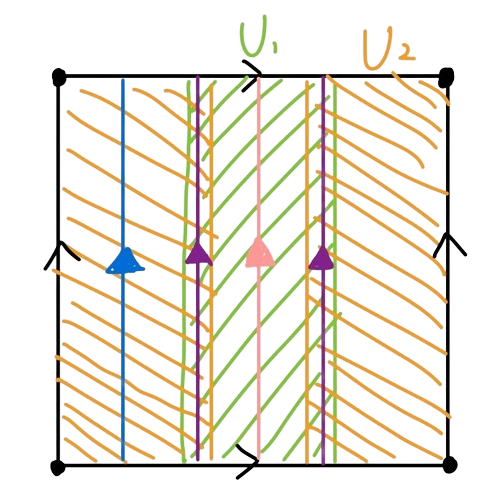
\includegraphics[scale = 0.3]{Image 1}
\end{center}

The two open sets $U_1,U_2$ each deformation retract to a circle and $U_1\cap U_2$ deformation retracts to a disjoint union of two circles. Using homotopy invariance, we obtain $$H_k(U_1),H_k(U_2)\cong\begin{cases}
\Z & \text{ if } k=0,1\\
0 & \text{ otherwise }
\end{cases}$$ and since the disjoint union of two circles consists of two path connected components, together with proposition 3.1.7, we have that $$H_k(U_1\cap U_2)\cong\begin{cases}
\Z\oplus\Z & \text{ if } k=0,1\\
0 & \text{ otherwise }
\end{cases}$$
By the Mayer-Vietoris sequence, the non-trivial terms of the sequence are precisely given by \\~\\
\adjustbox{scale=0.95,center}{\begin{tikzcd}
	0 & {\tilde{H}_2(T)} & {\tilde{H}_1(U_1\cap U_2)} & {\tilde{H}_1(U_1)\oplus \tilde{H}_2(U_2)} & {\tilde{H}_1(T)} & {\tilde{H}_0(U_1\cap U_2)} & 0
	\arrow[from=1-1, to=1-2]
	\arrow["\partial", from=1-2, to=1-3]
	\arrow["i", from=1-3, to=1-4]
	\arrow["j", from=1-4, to=1-5]
	\arrow["\partial", from=1-5, to=1-6]
	\arrow[from=1-6, to=1-7]
\end{tikzcd}}\\~\\
where $\partial$ are the connecting homomorphisms, $i$ and $j$ are induced by the inclusion maps $i=(\iota_1)_\ast-(\iota_2)_\ast$ and $j=(j_1)_\ast+(j_2)_\ast$. Also because $U_1,U_2$ and $T$ are all path connected the end terms are $0$. Rewriting them into known homology groups, we obtain \\~\\
\adjustbox{scale=1,center}{\begin{tikzcd}
	0 & {\tilde{H}_2(T)} & {\Z^2} & {\Z^2} & {\tilde{H}_1(T)} & {\Z} & 0
	\arrow[from=1-1, to=1-2]
	\arrow["\partial", from=1-2, to=1-3]
	\arrow["i", from=1-3, to=1-4]
	\arrow["j", from=1-4, to=1-5]
	\arrow["\partial", from=1-5, to=1-6]
	\arrow[from=1-6, to=1-7]
\end{tikzcd}}\\~\\
Consider the sequence \\~\\
\adjustbox{scale=1,center}{\begin{tikzcd}
	0 & {\tilde{H}_2(T)} & {\Z^2} & {\im(i)} & 0
	\arrow[from=1-1, to=1-2]
	\arrow["\partial", from=1-2, to=1-3]
	\arrow["i", from=1-3, to=1-4]
	\arrow[from=1-4, to=1-5]
\end{tikzcd}}\\~\\
This sequence is exact by definition. Moreover, since $\im(i)$ is a subgroup of the abelian group $\Z^2$, $\im(i)$ is finite free and so is isomorphic to $\Z^n$ for some $0\leq n\leq 2$. Then by proposition 1.2.6, the sequence is split exact and by proposition 1.2.5, we obtain that $$\Z^2\cong\tilde{H}_2(T)\oplus\im(i)$$ Since $\im(i)$ is a subgroup of $\Z^2$ we can divide both sides by $\im(i)$ to obtain $$\tilde{H}_2(T)\cong\frac{\Z^2}{\im(i)}\cong\ker(i)$$ Also, by considering the split exact sequence \\~\\
\adjustbox{scale=1,center}{\begin{tikzcd}
	0 & {\ker(\partial)} & {\tilde{H}_1(T)} & \Z & 0
	\arrow[from=1-1, to=1-2]
	\arrow["\iota", from=1-2, to=1-3]
	\arrow["\partial", from=1-3, to=1-4]
	\arrow[from=1-4, to=1-5]
\end{tikzcd}}\\~\\
we obtain an isomorphism $\tilde{H}_1(T)\cong\Z\oplus\ker(\partial)$. Now $\ker(\partial)=\im(j)$ since the sequence is exact. Also, we have that $$\frac{\Z^2}{\ker(j)}\cong\im(j)$$ by the first isomorphism theorem. Using the fact that the sequence being exact implies $\im(i)=\ker(j)$, we have that $$\tilde{H}_1(T)\cong\Z\oplus\im(j)\cong\Z\oplus\frac{\Z^2}{\ker(j)}\cong\frac{\Z^2}{\im(i)}\cong\Z\oplus\text{coker}(i)$$ We know have to compute what $i$ does to the generators of $\tilde{H}_1(U_1\cap U_2)\cong\Z$ marked in purple. Recall that $i$ is defined as $(\iota_1)_\ast-(\iota_2)_\ast$. $i$ then sends the generators to the positive generator (pink) in $U_1$. It sends the generators also to the positive generator (blue) in $U_2$. This means that our map $i$ can be written as $$i=\begin{pmatrix}
1 & 1\\
1 & 1
\end{pmatrix}$$ with basis vectors the two generators in $\tilde{H}_1(U_1\cap U_2)$ and the two in $\tilde{H}_1(U_1)\oplus\tilde{H}_2(U_2)$. The smith normal form of this map reduces it to the matrix $$\begin{pmatrix}
1 & 0\\
0 & 0
\end{pmatrix}$$ Its kernel is one copy of $\Z$ and its cokernel is also one copy of $\Z$. Thus we conclude that $$H_k(\T)=\begin{cases}
\Z & \text{if } k=0,2\\
\Z^2 & \text{if } k=1\\
0 & \text{otherwise}
\end{cases}$$
and so we are done. 
\end{proof}
\end{eg}

Note that the choice of the orientation of the generators is arbitrary, one can choose the opposite orientation and deduce the same homology groups. 

\begin{eg}{}{} Let $K$ denote the Klein bottle. Then the homology of the Klein bottle $K$ is $$H_k(K)=\begin{cases}
\Z & \text{if } k=0\\
\Z\oplus\Z/2\Z & \text{if } k=1\\
0 & \text{otherwise}
\end{cases}$$
\end{eg}

\subsection{Three Applications of Singular Homology}
In Algebraic Topology 1, we have seen Brouwer fixed point theorem for $D$ the unit disc in $\R^2$. Using homology groups, we can finally state and prove the result for $n$-dimensional discs. 

\begin{lmm}{}{} For any $k\in\N$, $S^{k-1}$ is not a retract of $D^k$. \tcbline
\begin{proof}
Assume to the contrary that $i:S^{k-1}\hookrightarrow D^k$ admits a retraction $r:D^k\to S^{k-1}$. Then $\text{id}_{S^k}=r\circ i$ so that \\~\\
\adjustbox{scale=1.0,center}{\begin{tikzcd}
	{\widetilde{H}_{k-1}(S^{k-1})} & {\widetilde{H}_{k-1}(D^k)} & {\widetilde{H}_{k-1}(S^{k-1})}
	\arrow["{i_\ast}", from=1-1, to=1-2]
	\arrow["{r_\ast}", from=1-2, to=1-3]
\end{tikzcd}}\\~\\
is the identity map. Substituting the homology of $S^{k-1}$ and $D^k$, we have that \\~\\
\adjustbox{scale=1.0,center}{\begin{tikzcd}
	\Z & 0 & \Z
	\arrow["{r_\ast}", from=1-2, to=1-3]
	\arrow["{i_\ast}", from=1-1, to=1-2]
\end{tikzcd}}\\~\\
is the identity map which is impossible. 
\end{proof}
\end{lmm}

\begin{thm}{Brouwer Fixed-point Theorem}{} Every continuous map $f:D^k\to D^k$ has a fixed point. \tcbline
\begin{proof}
Suppose not, then the ray starting at $f(x)$ in the direction of $x$ meets $S^{k-1}$ in exactly one point $g(x)\neq f(x)$. Then $g:D^k\to S^{k-1}$ defines a retraction. By the above corollary, this is a contradiction. 
\end{proof}
\end{thm}

Using topological properties preserved by homeomorphisms, we are only able to prove that $\R^1$ and $\R^2$ are not homeomorphic using the argument on the number of connected components. Using homology, we can prove the full form of invariance of domain. 

\begin{crl}{Invariance of Domain}{} If $n\neq m$, then $\R^n$ is not isomorphic $\R^m$. \tcbline
\begin{proof}
Assume that $\R^n\cong\R^m$. Then $f:\R^n\setminus\{0\}\to\R^m\setminus\{0\}$ is also a homeomorphism. Since $\R^n\setminus\{0\}\simeq S^{n-1}$ and $\R^m\setminus\{0\}\simeq S^{m-1}$, we have that $f_\ast$ induces an isomorphism $$\Z\cong\widetilde{H}_{n-1}(S^{n-1})\cong\widetilde{H}_{n-1}(S^{m-1})$$ by homotopy invariance and the computation of the homology groups of the $n$-sphere. This can only be true when $n=m$ by our computations. 
\end{proof}
\end{crl}

The Jordan curve theorem is a highly non-trivial result that looks deceptively easy to prove. Using homology we can give an algebraic proof. 

\begin{defn}{Jordan Curve}{} A Jordan Curve is a simple closed curve in $\R^2$. 
\end{defn}

\begin{lmm}{}{} Let $\gamma:I\to S^2$ be an injective continuous map with image $C=\gamma(I)$. Then $$H_n(S^2\setminus C)=\begin{cases}
\Z & \text{ if } n=0\\
0 & \text{ otherwise}
\end{cases}$$ \tcbline
\begin{proof}
Let $J\subseteq I$ be an interval. Define $C_J=\gamma(J)$. Let $U=S^2\setminus C_{[0,1/2]}$ and $V=S^2\setminus C_{[1/2,1]}$. Note that $U\cap V=S^2\setminus C$ and $$U\cup V=S^2\setminus C_{[1/2,1/2]}\cong\R^2\simeq\ast$$ By Mayer-Vietoris, we obtain isomorphisms $$H_n(S^2\setminus C)\cong H_n(S^2\setminus C_{[0,1/2]})\oplus H_n(S^2\setminus C_{[1/2,1]})$$ for $n\geq 1$ together with a short exact sequence \\~\\
\adjustbox{scale=1.0,center}{\begin{tikzcd}
	0 & {H_0(S^2\setminus C)} & {H_0(S^2\setminus C_{[0,1/2]})\oplus H_0(S^2\setminus C_{[1/2,1]})} & \Z & 0
	\arrow[from=1-1, to=1-2]
	\arrow[from=1-2, to=1-3]
	\arrow[from=1-3, to=1-4]
	\arrow[from=1-4, to=1-5]
\end{tikzcd}}\\~\\
Assume for a contradiction that for some $n\geq 1$ there exists $\sigma\in H_n(S^2\setminus C)$ which is non-zero. By the isomorphism above, it remains non-zero in one of the two groups of the direct sum. By repeating this argument cutting the interval where its homology group contains $\sigma$ in half, we obtain a nested sequence of intervals $$I\supset J_1\supset J_2\supset\cdots$$ with non zero intersection $p\in\bigcap_{i=1}^\infty J_i$ such that $\sigma\neq 0$ in all of $H_n(S^2\setminus C_{J_l})$. However we have that $S^2\setminus C_{[p,p]}\cong\R^2$ is contractible hence $\sigma$ vanishes in $H_n(S^2\setminus\{\gamma(p)\})$. Let $\tau\in C_{n+1}(S^2\setminus C_{[p,p]}$ such that $\partial\tau=\sigma$. Write $\tau$ as a finite linear combination of singular simplexes. Each of the singular simplexes has compact image in $S^2\setminus C_{[p,p]}$ since $\Delta^{n+1}$ is compact. The union of these images is covered by open subsets $(S^2\setminus C_{J_l})_l$ so by compactness, there exists $l$ such that $\tau\in C_{n+1}(S^2\setminus C_{J_l})$. But then $\sigma=0$ in $H_n(S^2\setminus C_{J_l})$, which is a contradiction. Thus $H_n(S^2\setminus C)=0$ for all $n\geq 1$. \\~\\

For $n=0$, assume that $x,y\in S^2\setminus C$ are distinct in different path components. Then similar to the above we obtain a nested sequence of intervals $J_l$ such that $x$ and $y$ are in different path components of $S^2\setminus C_{J_l}$ for all $l$. Since $S^2\setminus\{\gamma(p)\}$ is contractible, it must contain a path connecting $x$ and $y$. By compactness, this path misses $C_{J_l}$ for large $l$. Thus $x$ and $y$ lie in the same path component of $S^2\setminus C_{J_l}$ for large $l$, which is a contradiction. We deduce that $H_0(S^2\setminus C)=\Z$. 
\end{proof}
\end{lmm}

\begin{thm}{Jordan Curve Theorem}{} Let $\gamma:[0,1]\to\R^2$ be a Jordan curve with image $C$. Then $\R^2\setminus C$ has two connected components.  \tcbline
\begin{proof}
Choose $S_+^1$ and $S_-^1$ the upper and lower hemicircles of $S^1$ so that the intersection is $S^0$. Define the following: $X=S^2\setminus\gamma(S^0)$, $U_+=S^2\setminus\gamma(S_+^1)$, $U_-=S^2\setminus\gamma(S_-^1)$ and $U_+\cap U_-=S^2\setminus C$. Since $S_\pm^1\cong I$, the homology groups of $U_\pm$ is given by the above lemma. Also $X\simeq S^1$. By Mayer-Vietoris applied to $U,V,X$, we obtain an exact sequence \\~\\
\adjustbox{scale=1.0,center}{\begin{tikzcd}
	0 & {H_{n+1}(S^2\setminus\gamma(S^0))} & {H_n(S^2\setminus C)} & {H_n(U_+)\oplus H_n(U_-)}
	\arrow[from=1-1, to=1-2]
	\arrow[from=1-2, to=1-3]
	\arrow[from=1-3, to=1-4]
\end{tikzcd}}\\~\\
for $n>0$ in which the first and third term vanish so that $H_n(S^2\setminus C)=0$. For $n=0$, we have an exact sequence \\~\\
\adjustbox{scale=1.0,center}{\begin{tikzcd}
	0 & {H_{1}(S^2\setminus\gamma(S^0))} & {\widetilde{H}_0(S^2\setminus C)} & {\widetilde{H}_0(U_+)\oplus\widetilde{H}_0(U_-)}
	\arrow[from=1-1, to=1-2]
	\arrow[from=1-2, to=1-3]
	\arrow[from=1-3, to=1-4]
\end{tikzcd}}\\~\\
where the last term vanishes. Thus we have an isomorphism $\widetilde{H}_0(S^2\setminus C)\cong\Z$. It follows that $H_0(S^2\setminus C)\cong\Z^2$. So now we have $$H_n(S^2\setminus C)=\begin{cases}
\Z^2 & \text{ if } n=0\\
0 & \text{ otherwise }
\end{cases}$$

Now consider $X=S^2\setminus C$ and $U=\R^2\setminus C$ identified in $\R^2\cup\{\infty\}\cong S^2$. Let $V$ be an open disk around $\infty$ that does not meet $C$. Using Mayer-Vietoris sequence, the only interesting terms are this sequence \\~\\
\adjustbox{scale=1.0,center}{\begin{tikzcd}
	0 & {H_n(\R^2\setminus C)} & 0
	\arrow[from=1-1, to=1-2]
	\arrow[from=1-2, to=1-3]
\end{tikzcd}}\\~\\
for $n\geq 2$, which gives $H_n(\R^2\setminus C)=0$ and the lower degree terms give an exact sequence \\~\\
\adjustbox{scale=1.0,center}{\begin{tikzcd}
	0 & \Z & {H_1(\R^2\setminus C)} & 0 & 0 & {\widetilde{H}_0(\R^2\setminus C)} & \Z & 0
	\arrow[from=1-1, to=1-2]
	\arrow[from=1-2, to=1-3]
	\arrow[from=1-3, to=1-4]
	\arrow[from=1-4, to=1-5]
	\arrow[from=1-5, to=1-6]
	\arrow[from=1-6, to=1-7]
	\arrow[from=1-7, to=1-8]
\end{tikzcd}}\\~\\
which is due to the fact that $U\cap V\simeq S^1$ and $V$ is contractible. Then it is clear that $H_1(\R^2\setminus C)\cong\Z$ and $\widetilde{H}_0(\R^2\setminus C)\cong\Z$ so that $H_0(\R^2\setminus C)\cong\Z^2$ and so we obtain $$H_n(\R^2\setminus C)=\begin{cases}
\Z^2 & \text{ if } n=0\\
\Z & \text{ if } n=1\\
0 & \text{ if } n>1
\end{cases}$$
Since $\R^2\setminus C$ is locally path connected, by corollary 3.2.3 we thus have that $\R^2\setminus C$ has two connected components. 
\end{proof}
\end{thm}

\pagebreak
\section{Relative Homology}
\subsection{Relative Homology Groups}
Given a subspace $A$ of a space $X$, we know that the inclusion map $A\hookrightarrow X$ induces an inclusion $C_n(A)\hookrightarrow C_n(X)$. Unfortunately, this does not induce an injection $H_n(A)\to H_n(X)$. Relative homology gives a precise measure of the failure of injectivity and surjectivity of the map in homology. 

\begin{defn}{Relative Homology Group}{} Let $X$ be a topological space and $A\subseteq X$ a subspace. Define the relative homology group $H_n(X,A)$ to be the homology group of the chain complex \\~\\
\adjustbox{scale=1.1,center}{\begin{tikzcd}
\cdots\arrow[r] & C_n(X,A)\arrow[r, "\partial"] & C_{n-1}(X,A)\arrow[r] & \cdots
\end{tikzcd}}\\~\\
where $C_n(X,A)$ denotes the quotient group $C_n(X)/C_n(A)$. In other words, $$H_n(X,A)=\frac{\ker(\partial:C_n(X,A)\to C_{n-1}(X,A))}{\im(\partial:C_{n+1}(X,A)\to C_n(X,A))}=H_n(C_\bullet(X,A))$$~\\
Elements of $Z_n(X,A)$ are called relative $n$-cycles, while elements of $B_n(X,A)$ are called relative $n$-boundaries. 
\end{defn}

Geometrically, relative $n$-cycles are $n$-cycles in $C_n(X)$ such that $\partial z\in C_{n-1}(A)$ which means that the boundary of $z$ is contained in the subspace $A$. Intuitively, we are treating cycles in the subspace $A$ as $0$ and so the homology groups measure the homology of $X$ without $A$. 

\begin{thm}{Exact Sequence of Pairs of Spaces}{} Let $(X,A)$ be a pair of spaces. Then there is an exact sequence \\~\\
\adjustbox{scale=1.0,center}{\begin{tikzcd}
\cdots\arrow[r] & H_n(A)\arrow[r, "\iota_\ast"] & H_n(X)\arrow[r, "j_\ast"] & H_n(X,A)\arrow[r, "\partial"] & H_{n-1}(A)\arrow[r] & \cdots
\end{tikzcd}}\\~\\
where 
\begin{itemize}
\item $\iota:A\to X$ is the inclusion map
\item $j:X\to X\setminus A$ is the quotient map
\item The connecting homomorphism $\partial:H_n(X,A)\to H_{n-1}(A)$ is defined by $[z]\mapsto[dz]$ for $z\in C_n(X)$ a relative cycle. 
\end{itemize}
Moreover, the exact sequence is natural with respect to maps $f:(X,A)\to(Y,B)$. \tcbline
\begin{proof}
Notice that \\~\\
\adjustbox{scale=1.0,center}{\begin{tikzcd}
0\arrow[r] & C_\bullet(A)\arrow[r, "\iota"] & C_\bullet(X)\arrow[r, "j"] & C_\bullet(X,A)\arrow[r] & 0
\end{tikzcd}}\\~\\
is a short exact sequence by construction. Thus it induces a long exact sequence in homology groups. \\~\\

Consider $[z]=z+C_n(A)\in C_n(X,A)$ a cycle in $C_n(X,A)$. The surjective map $j$ is the projection map so $j(z)=[z]$. Now $d(z)\in\ker(j)$ because $$j(d(z))=d(j(z))=d([z])=0$$ by assumption So $d(z)\in\ker(j)=\im(i)$. Since $i$ is the inclusion, $[d(z)]\in C_{n-1}(A)$ is precisely the element that $\partial$ maps $[z]$ to. 
\end{proof}
\end{thm}

We obtain an immediate result of the singular homology of the space $X$ and its subspace $A$. 

\begin{lmm}{}{} Let $(X,A)$ be a pair of spaces. The inclusion map $\iota:A\to X$ induces an isomorphism $$H_n(A)\cong H_n(X)$$ for all $n\in\N$ if and only if $H_n(X,A)=0$ for all $n$. \tcbline
\begin{proof}
If $H_n(X,A)=0$ for all $n\in\N$, then the long exact sequence above shows that there are isomorphisms $H_n(A)\cong H_n(X)$. If $H_n(A)\cong H_n(X)$ in the long exact sequence above, then the map $H_n(X)\to H_n(X,A)$ is the zero map and the map $H_n(X,A)\to H_{n-1}(A)$ is the zero map. Thus for $n\geq 0$ there is an exact sequence \\~\\
\adjustbox{scale=1.0,center}{\begin{tikzcd}
	0 & {H_n(X,A)} & 0
	\arrow[from=1-1, to=1-2]
	\arrow[from=1-2, to=1-3]
\end{tikzcd}}\\~\\
showing that $H_n(X,A)=0$. 
\end{proof}
\end{lmm}

Notice that relative homology is more generalized than reduced homology in the following sense: 

\begin{lmm}{}{} Let $X$ be space and $x\in X$ be a point. Then there is an isomorphism $$H_n(X,x)\cong\widetilde{H}_n(X)$$ of homology groups for all $n\in\N$. \tcbline
\begin{proof}
We have a long exact sequence as in theorem 4.1.3. In particular, since $H_n(\{x\})=0$ for all $n\geq 1$, we have an isomorphism $$H_n(X,x)\cong H_n(X)$$ which descends to an isomorphism in reduced homology. We are now left with the exact sequence: \\~\\
\adjustbox{scale=1.0,center}{\begin{tikzcd}
0\arrow[r] & H_1(X)\arrow[r, "j_\ast"] & H_1(X,x)\arrow[r, "\partial"] & H_0(x)\arrow[r, "\iota_\ast"] & H_0(X)\arrow[r, "j_\ast"] & H_0(X,x)\arrow[r] & 0
\end{tikzcd}}\\~\\
Now since $\iota:\{x\}\to X$ is the inclusion map, the projection map $p:X\to\{x\}$ is such that $p\circ\iota=\text{id}$. By proposition 3.1.6 we have $p_\ast\circ\iota_\circ=\text{id}_\ast$ and thus $\iota_\ast$ is injective and has kernel $0$. Exactness then implies that $\im(\partial)=\ker(\iota_\ast)=0$ and thus $\partial$ is the zero map. This means that $\tilde{H}_1(X)\cong H_1(X)\cong H_1(X,x)$. \\~\\

We are now left with a short exact sequence\\~\\
\adjustbox{scale=1.0,center}{\begin{tikzcd}
0\arrow[r] & \Z\arrow[r, "\iota_\ast"] & H_0(X)\arrow[r, "j_\ast"] & H_0(X,x)\arrow[r] & 0
\end{tikzcd}}\\~\\
Since $H_0(\ast)\cong\Z$. The map $p_\ast:H_0(X)\to H_0(x)$ has the property that $p_\ast\circ\iota_\ast=\text{id}_\ast$. This means that the short exact sequence is split exact and we have that $$H_0(X)\cong\Z\oplus H_0(X,x)$$ Consider the map \\~\\
\adjustbox{scale=1.0,center}{\begin{tikzcd}
H_0(X)\arrow[r, "p_\ast\times j_\ast", "\cong"'] & H_0(x)\oplus H_0(X,x)\arrow[r, "\pi"] & H_0(x)
\end{tikzcd}}\\~\\
where $\pi:H_0(x)\oplus H_0(X,x)\to H_0(x)$ is defined by $\pi(a,c)=a$. This map sends $b\in H_0(X)$ to $p_\ast(b)$. Then we have 
\begin{align*}
\widetilde{H}_0(X)&\cong\ker(H_0(X)\to H_0(x))\\
&\cong\ker(H_0(X)\oplus H_0(X,x)\overset{p_\ast}{\to}H_0(x))\\
&=H_0(X,x)
\end{align*}
Therefore we conclude. 
\end{proof}
\end{lmm}

Relative homology also satisfies the homotopy invariance property and has the Mayer-Vietoris sequence. 

\begin{thm}{Homotopy Invariance}{} Let $(X,A),(Y,B)$ be pairs of spaces. Let $f,g:(X,A)\to(Y,B)$ be homotopic maps. Then the induced map on relative homology are the same: $$f_\ast=g_\ast:H_n(X,A)\to H_n(Y,B)$$ 
\end{thm}

\begin{crl}{}{} Let $f:(X,A)\to (Y,B)$ be a map such that both $f:X\to Y$ and $f|_A:A\to B$ are homotopy equivalences. Then $$f_\ast:H_n(X,A)\to H_n(Y,B)$$ induces an isomorphism for all $n\in\N$. 
\end{crl}

\begin{prp}{Long Exact Sequence of a Triple}{} Let $(X,A,B)$ be a triplet of space such that $B\subset A\subset X$. Then \\~\\
\adjustbox{scale=1.0,center}{\begin{tikzcd}
	0 & {C_n(A,B)} & {C_n(X,B)} & {C_n(X,A)} & 0
	\arrow[from=1-1, to=1-2]
	\arrow[from=1-2, to=1-3]
	\arrow[from=1-3, to=1-4]
	\arrow[from=1-4, to=1-5]
\end{tikzcd}}\\~\\
is a short exact sequence that gives rise to a long exact sequence \\~\\
\adjustbox{scale=1.0,center}{\begin{tikzcd}
	\cdots & {H_n(A,B)} & {H_n(X,B)} & {H_n(X,A)} & {H_{n-1}(A,B)} & \cdots
	\arrow[from=1-1, to=1-2]
	\arrow[from=1-2, to=1-3]
	\arrow[from=1-3, to=1-4]
	\arrow[from=1-4, to=1-5]
	\arrow[from=1-5, to=1-6]
\end{tikzcd}}\\~\\
in relative homology. Moreover, the exact sequence is natural with respect to maps $f:(X,A,B)\to(Y,C,D)$. 
\end{prp}

\begin{thm}{Relative Mayer-Vietoris Sequence}{} Let $(X,Y)$ be a pair of space such that $A,B\subset X$ cover $X$ and $C,D\subset Y$ cover $Y$ with $C\subset A$ and $D\subset B$. Then there is an exact sequence \\~\\
\adjustbox{scale=1.0,center}{\begin{tikzcd}
	\cdots & {H_n(A\cap B,C\cap D)} && {H_n(A,C)\oplus H_n(B,D)} && {H_n(X,Y)} & \cdots
	\arrow[from=1-1, to=1-2]
	\arrow["\Phi", from=1-2, to=1-4]
	\arrow["\Psi", from=1-4, to=1-6]
	\arrow[from=1-6, to=1-7]
\end{tikzcd}}\\~\\
in relative homology. 
\end{thm}

Using the lemma, we have a low degree interpretation for relative homology. 

\begin{prp}{}{} Let $(X,A)$ be a pair of space. Then the following are true. 
\begin{itemize}
\item $H_0(X,A)=0$ if and only if every path component of $X$ contains at least one path component of $A$. 
\item $H_1(X,A)=0$ if and only if $H_1(A)\to H_1(X)$ is surjective and each path component of $X$ contains at most one path-component of $A$. 
\end{itemize}
\end{prp}

\subsection{Quotient Spaces and Excision}
The excision theorem is a powerful theorem for computing relative homology groups. This statement is derived directly from Mayer-Vietoris. 

\begin{thm}{The Excision Theorem}{} Let $X$ be a space and $Z,A$ be subspaces of $X$ such that $\overline{Z}\subseteq A^\circ$. Then the inclusion map $(X\setminus Z,A\setminus Z)\hookrightarrow (X,A)$ induces an isomorphism $$H_n(X\setminus Z,A\setminus Z)\cong H_n(X,A)$$ for all $n$. Moreover, the excision isomorphism is natural in maps $f:(X,A,Z)\to(Y,B,C)$. \tcbline
\begin{proof}
Let $B=X\setminus Z$. Then notice that $A\cap B=A\setminus Z$, $A^\circ\cup B^\circ=A^\circ\cup(X\setminus\overline{Z})=X$. Moreover, we have that 
\begin{align*}
C_n(X\setminus Z,A\setminus Z)&=C_n(B,A\cap B)\\
&=\frac{C_n(B)}{C_n(A\cap B)}\tag{By definition}\\
&\cong\frac{C_n(A+B)}{C_n(A)}\tag{Second Isomorphism Theorem}
\end{align*}
This implies that \\~\\
\adjustbox{scale=1.0,center}{\begin{tikzcd}
0\arrow[r] & C_\bullet(A)\arrow[r] & C_\bullet(A+B)\arrow[r] & C_\bullet(X\setminus Z,A\setminus Z)\arrow[r] & 0
\end{tikzcd}}\\~\\
is a short exact sequence of chain complexes. Moreover, by considering inclusion maps, we have the following commutative diagram: \\~\\
\adjustbox{scale=1.0,center}{\begin{tikzcd}
0\arrow[r] & C_\bullet(A)\arrow[r]\arrow[d, "="] & C_\bullet(A+B)\arrow[r]\arrow[d] & C_\bullet(X\setminus Z,A\setminus Z)\arrow[r]\arrow[d] & 0\\
0\arrow[r] & C_\bullet(A)\arrow[r] & C_\bullet(X)\arrow[r] & C_\bullet(X,A)\arrow[r] & 0
\end{tikzcd}}\\~\\
Considering that the rows are short exact sequences of chain complexes, they induce long exact sequences in homology by naturality in theorem 1.4.3: \\~\\
\adjustbox{scale=0.9,center}{\begin{tikzcd}
\cdots\arrow[r] & H_n(A)\arrow[r]\arrow[d, "="] & H_n(A+B)\arrow[r]\arrow[d] & H_n(X\setminus Z,A\setminus Z)\arrow[r]\arrow[d] & H_{n-1}(A)\arrow[r]\arrow[d, "="] & H_{n-1}(A+B)\arrow[r]\arrow[d] & \cdots\\
\cdots\arrow[r] & H_n(A)\arrow[r] & H_n(X)\arrow[r] & H_n(X,A)\arrow[r] & H_{n-1}(A)\arrow[r] & H_{n-1}(X)\arrow[r] & \cdots
\end{tikzcd}}\\~\\
where the vertical arrows are naturally induced by inclusion. By proposition 8.2.3, the second the fifth arrows are isomorphisms. Thus by the five lemma, we have that $$H_n(X\setminus Z,A\setminus Z)\cong H_n(X,A)$$ and so we are done. 
\end{proof}
\end{thm}

\begin{lmm}{}{} The Excision Theorem is equivalent to the following version: If $A,B\subset X$ are subspaces such that $X=A^\circ\cup B^\circ$, then the inclusion $(B,A\cap B)\to (X,A)$ induces isomorphisms $$H_n(B,A\cap B)\overset{\cong}{\longrightarrow} H_n(X,A)$$ for all $n$. 
\end{lmm}

When $X$ and $A$ in relative homology is nice enough, we can interpret the result from relative homology as the homology groups of the quotient space. The following notation is due to Hatcher. 

\begin{defn}{Good Pairs}{} Let $X$ be a space and $A$ a closed subspace of $X$. We say that the pair $(X,A)$ is a good pair if there exists an open set $V$ such that $A\subset V$ and $V$ deformation retracts to $A$. 
\end{defn}

It is clear by definition that any CW-complex $X$ and subcomplex $A$ forms a good pair. 

\begin{lmm}{}{} Both CW-complexes and $\Delta$-complexes are good pairs. 
\end{lmm}

\begin{prp}{}{} Let $X$ be a space and $A$ a closed subspace of $X$ such that $(X,A)$ is a good pair. Then the quotient map $X\to X/A$ induces a natural isomorphism $$H_n(X,A)\cong H_n(X/A,A/A)\cong\widetilde{H}_n(X/A)$$ in homology groups. \tcbline
\begin{proof}
Let $V$ be a open neighbourhood of $A$ satisfying the good pair condition. Then there is an obvious inclusion map $(X,A)\to(X,V)$. Applying the long exact sequence of relative homology for both $(X,A)$ and $(X,V)$, we obtain the following diagram by naturality in theorem 1.4.3: \\~\\
\adjustbox{scale=1.0,center}{\begin{tikzcd}
	\cdots & {H_n(A)} & {H_n(X)} & {H_n(X,A)} & {H_{n-1}(A)} & {H_{n-1}(X)} & \cdots \\
	\\
	\cdots & {H_n(V)} & {H_n(X)} & {H_n(X,V)} & {H_{n-1}(V)} & {H_{n-1}(X)} & \cdots
	\arrow[from=1-1, to=1-2]
	\arrow[from=1-2, to=1-3]
	\arrow["\cong"{description}, from=1-2, to=3-2]
	\arrow[from=1-3, to=1-4]
	\arrow["\cong"{description}, from=1-3, to=3-3]
	\arrow[from=1-4, to=1-5]
	\arrow[from=1-4, to=3-4]
	\arrow[from=1-5, to=1-6]
	\arrow["\cong"{description}, from=1-5, to=3-5]
	\arrow[from=1-6, to=1-7]
	\arrow["\cong"{description}, from=1-6, to=3-6]
	\arrow[from=3-1, to=3-2]
	\arrow[from=3-2, to=3-3]
	\arrow[from=3-3, to=3-4]
	\arrow[from=3-4, to=3-5]
	\arrow[from=3-5, to=3-6]
	\arrow[from=3-6, to=3-7]
\end{tikzcd}}\\~\\
where the isomorphisms come from the fact that $V$ deformation retracts onto $V$ since $(X,A)$ is a good pair. By the five lemma, we obtain an isomorphism $$H_n(X,A)\cong H_n(X,V)$$ By excision, we obtain another isomorphism $$H_n(X,A)\cong H_n(X,V)\cong H_n(X\setminus A,V\setminus A)$$ Repeating the argument with $(X/A,A/A)$, we obtain an isomorphism $$H_n(X/A,A/A)\cong H_n(X\setminus A,V\setminus A)\cong H_n\left(\left(\frac{X}{A}\right)\setminus\left(\frac{A}{A}\right),\left(\frac{V}{A}\right)\setminus\left(\frac{A}{A}\right)\right)$$ Combining the two gives the desired result. 
\end{proof}
\end{prp}

Most pairs of spaces are good pairs. We provide some examples that are not. \\~\\

The Hawaiian earrings with its wedge point is not a good pair since any open neighbourhood of the wedge point contains an infinite number of circles and so cannot be contractible. \\~\\

The interval together with $A=\left\{\frac{1}{n}\;|\;n\in\N\setminus\{0\}\right\}$ is not a good pair. In fact, one can show that the pair $(X/A,A/A)$ is homeomorphic to the Hawaiian earring with the wedge point. 

\begin{prp}{}{} Let $k\geq 0$, we have that $$H_n(\Delta^k,\partial\Delta^k)=\begin{cases}
\Z & \text{ if } n=k\\
0 & \text{ otherwise }
\end{cases}$$ \tcbline
\begin{proof}
Since $\Delta^k$ is also a CW-complex, $(\Delta^k,\partial\Delta^k)$ is a good pair thus we can apply proposition 6.2.4 to obtain $$\widetilde{H}_n(\Delta^k,\partial\Delta^k)\cong\tilde{H}_n(S^k)$$ and so the desired results follows. 
\end{proof}
\end{prp}

\begin{lmm}{}{} Assume that each $(X_i,x_i)$ is a good pair. Then we have an isomorphism $$\widetilde{H}_n\left(\bigvee_{i\in I}(X_i,x_i)\right)=\bigoplus_{i\in I}\widetilde{H}_n(X_i)$$ in reduced homology. 
\end{lmm}

\subsection{Local Homology Groups}
Local homology groups forgets every homological information about the space $X$, under than a small neighbourhood around some subset $A\subseteq X$. 

\begin{defn}{The Local Homology Groups}{} Let $X$ be a space. Let $A\subseteq X$ be a subspace. Define the local homology group of $X$ in $A$ to be the homology groups $$H_n(X\;|\;A)=H_n(X,X\setminus A)$$ for each $n\in\N$. 
\end{defn}

Elements of the local homology group are represented by cycles in $X$ whose boundary lie outside of $x$. It is called local because it only captures local topological data of $X$ surrounding $x$. 

\begin{prp}{}{} For all $n,k\in\N$, there is an isomorphism $$H_n(\R^k\;|\;\{\ast\})\cong\begin{cases}
\Z & \text{ if } n=k\\
0 & \text{ if } n\neq k
\end{cases}$$ \tcbline
\begin{proof}
Now if $k=0$, the results are clear. If $k\geq 1$, then the long exact sequence of the pair $(\R^k,\R^k\setminus\ast)$ together with the fact that $\R^k\setminus\ast\simeq S^{k-1}$ and $\R^k\simeq\ast$ gives $$H_n(\R^k\;|\;\ast)=0$$ for $n>k$ and $n<k$. When $n=k$, we have an exact sequence \\~\\
\adjustbox{scale=1.0,center}{\begin{tikzcd}
	0 & {H_k(\R^k\;|\;\ast)} & {H_{k-1}(S^{k-1})} & {H_{k-1}(\R^k)}
	\arrow[from=1-1, to=1-2]
	\arrow[from=1-2, to=1-3]
	\arrow[from=1-3, to=1-4]
\end{tikzcd}}\\~\\
when $k>1$ since $H_{k-1}(\R^k)=0$. Thus $H_k(\R^k\;|\;\ast)\cong\Z$. If $k=1$, then the last map $H_0(S^0)\to H_0(\R)$ is given by the matrix $\begin{pmatrix}
1 & 1
\end{pmatrix}:\Z^2\to\Z$ thus also giving isomorphism. 
\end{proof}
\end{prp}

The excision theorem gives the following stronger version of invariance of domain. 

\begin{crl}{}{} Let $U\subseteq\R^m$ and $V\subseteq\R^n$ be non empty open subsets. If $U\cong V$ then $m=n$. \tcbline
\begin{proof}
Let $x\in U$. By excision, we obtain an isomorphism $$H_k(U\;|\;\{x\})\cong H_k(\R^m\;|\;\{x\})\cong\begin{cases}
\Z & \text{ if } m=k\\
0 & \text{ if } n\neq k
\end{cases}$$ and similarly for $H_k(V\;|\;\{\phi(x)\})$ if $\phi:U\to V$ gives the homeomorphism. Then it is clear that if the homology groups are equal, then $m=n$. 
\end{proof}
\end{crl}

This shows that no connected manifold can have atlases mapping to different dimensions of $\R$ so that the notion of dimension is well defined. 

\pagebreak
\section{Degree Theory and Cellular Homology}
\subsection{Degree of Continuous Maps}
The degree is a main component of the explicit construction of maps in cellular homology. Therefore we develop some of the basic theory here. Degree theory is also an important subject in its own right. 

\begin{defn}{Degree of a Continuous Map}{} Let $f:S^k\to S^k$ be a continuous map. Let $$f_\ast:\widetilde{H}_k(S^k)\cong\Z\to\widetilde{H}_k(S^k)\cong\Z$$ be induced by $f$ and let $f_\ast(1)=n$. Define the degree of $f$ to be $\deg(f)=n$. 
\end{defn}

\begin{lmm}{}{} Let $f,g:S^k\to S^k$ be continuous maps. Then the following are true regarding the degree. 
\begin{itemize}
\item $\deg(\text{id})=1$
\item $\deg(g\circ f)=\deg(g)\cdot\deg(f)$
\item If $f\simeq g$ then $\deg(g)=\deg(f)$
\item If $f$ is a homotopy equivalence then $\deg(f)=\pm1$
\item If $f$ is not surjective then $\deg(f)=0$. 
\end{itemize} \tcbline
\begin{proof}~\\
\begin{itemize}
\item The identity map on the $k$-sphere induces the identity map on the homology groups. 
\item Direct consequence of functoriality of the induced map. 
\item Direct consequence of homotopy invariance. 
\item If $f$ is a homotopy equivalence that $f\simeq\text{id}$. By the third and first point we are done. 
\item Let $x\in S^k$ not be in the image of $f$. Then we obtain a factorization of $f$. \\~\\
\adjustbox{scale=1.0,center}{\begin{tikzcd}
	{S^k} && {S^k} \\
	& {S^k\setminus\{x\}}
	\arrow["f", from=1-1, to=1-3]
	\arrow[from=1-1, to=2-2]
	\arrow[from=2-2, to=1-3]
\end{tikzcd}}\\~\\
Passing to reduced homology, we see that $f_\ast$ factors through $0$: \\~\\
\adjustbox{scale=1.0,center}{\begin{tikzcd}
	{\Z} && {\Z} \\
	& {0}
	\arrow["f_\ast", from=1-1, to=1-3]
	\arrow[from=1-1, to=2-2]
	\arrow[from=2-2, to=1-3]
\end{tikzcd}}\\~\\
so that $f_\ast$ is the $0$ map. 
\end{itemize} 
and so we conclude. 
\end{proof}
\end{lmm}

It is easy to compute all the possible degrees when $k=0$ or $1$. When $k=0$, there are two points to map to and so there are two obvious maps: the identity and the continuous map taking one point to the other. Any other map must be homotopic to one of these two thus the only possible degree maps of $S^0$ is just the identity with degree $0$ and the non-trivial map with degree $1$. \\~\\

When $k=1$, the set of maps $f:S^1\to S^1$ defined by $z\mapsto z^n$ has degree $n$. Indeed from Algebraic Topology 1 we have seen that every $\omega_n:I\to S^1$ defined by $t\mapsto e^{2\pi int}$ induces a map of sending the generator in $H_1(S^1)\cong\pi_1(S^1,1)$ to $n$ times the generator. Explicitly, if $\sigma:I\to S^1$ is the generator in $H_1(S^1)$ defined by $\sigma(t)=e^{2\pi it}$, then $f\circ\sigma$ is homologous to $n\sigma$ again via $\pi_1(S^1,1)\cong H_1(S^1)$. 

\begin{prp}{}{} For all $k\geq 1$ and for all $n\in\Z$, there exists a continuous map $f:S^k\to S^k$ of degree $n$. \tcbline
\begin{proof}
Define $SX=\frac{X\times[-1,1]}{X\times\{-1\},X\times\{1\}}$ (the suspension of $X$). The two open sets $$C_+X=\frac{X\times(\epsilon,1]}{X\times\{1\}}\;\;\;\;\text{ and }\;\;\;\; C_-X=\frac{X\times[-1,\epsilon)}{X\times\{-1\}}$$ are contractible. By Mayer-Vietoris sequence, we obtain an isomorphism $$H_{k+1}(SX)\overset{\partial}{\cong}H_k(X)$$ It is clear that every map $f:X\to Y$ induces a map $Sf:SX\to SY$ by $Sf(x,t)=(f(x),t)$. Now notice that the following diagram \\~\\
\adjustbox{scale=1.0,center}{\begin{tikzcd}
	{H_{k+1}(SX)} & {H_{k+1}(SY)} \\
	{H_k(X)} & {H_k(Y)}
	\arrow["{Sf_\ast}", from=1-1, to=1-2]
	\arrow["\partial"', from=1-1, to=2-1]
	\arrow["\partial", from=1-2, to=2-2]
	\arrow["{f_\ast}"', from=2-1, to=2-2]
\end{tikzcd}}\\~\\
commutes by naturality in theorem 1.4.3. Applying this with $X=Y=S^{k-1}$ and since $S(S^{k-1})\cong S^k$, we deduce that $\deg(Sf)=\deg(f)$ so if we use induction, we are done. But the base case is already treated by the above paragraph, and so we conclude. 
\end{proof}
\end{prp}

Using the fundamental class of a sphere, we can compute the degree of a reflection. 

\begin{lmm}{}{} Let $S^k\subseteq\R^{k+1}$ be the unit circle. Let $f:S^k\to S^k$ be the reflection of a hyperplane through $0$ in $\R^{k+1}$. Then $\deg(f)=-1$. \tcbline
\begin{proof}
The top $S_+^k$ and bottom $S_-^k$ half of the sphere cut by the hyperplane  are homeomorphic to $k$-simplicies. Choose $k$-simplicies $\sigma_+:\Delta^k\overset{\cong}{\longrightarrow}S_+^k$ and $\sigma_-^k:\Delta^k\overset{\cong}{\longrightarrow}S_-^k$ such that $\partial\Delta^k$ is mapped homeomorphically to the equator $S_+^k\cap S_-^k$ in both cases, and that the composition $$\partial\Delta^k\overset{\sigma_+}{\longrightarrow}S_+^k\cap S_-^k\overset{(\sigma_-)^{-1}}{\longrightarrow}\partial\Delta^k$$ is the identity. \\~\\

It is clear that it is a cycle since it is a boundary in the chain complex $C_\bullet(\Delta^{k+1})$. I claim that $[\sigma_+-\sigma_-]$ is a generator of $H_k(S^k)$. \\~\\

We proceed by induction. When $k=0$, the statement is clear. So suppose that $k>0$. Let $U_1,U_2$ be open subspaces of $\Delta^{k+1}$ as follows. $U_1$ is an open neighbourhood of the last face of $\partial_{k+1}\Delta^{k+1}$ which deformation retracts onto $\partial\Delta^{k+1}$. $U_2$ is an open neighbourhood of the remaining faces $U_2=\bigcup_{i=0}^k\partial_i\Delta^{k+1}$ which deformation retracts onto $\bigcup_{i=0}^k\partial_i\Delta^{k+1}$. Moreover, choose them in such a way that $U_1\cap U_2$ deformation retract onto $\partial\partial\Delta^{k+1}=\partial[v_0,\dots,v_k]$ and $U_1\cup U_2$ deformation retracts onto $\partial[v_0,\dots,v_{k+1}]$. By induction hypothesis, we know that $\widetilde{H}_{k-1}(U_1\cap U_2)\cong\Z$ is generated by $$\partial([v_0,\dots,v_k])=\sum_{i=0}^k(-1)^i[v_0,\dots,\hat{v}_i,\dots,v_k]$$ From Mayer-Vietoris sequence, since $U_1\cup U_2$ deformation retracts onto $\partial\Delta^{k+1}$, the connecting homomorphism $$\widetilde{H}_k(U_1\cup U_2)\to\widetilde{H}_{k-1}(U_1\cap U_2)$$ since $U_1$ and $U_2$ are contractible so we only need to show that $\partial\sigma$ is sent to the generator or its negative. \\~\\

For this we will explicitly compute the connecting homomorphism. It is clear that $$\left((-1)^{k+1}[v_0,\dots,v_k],\sum_{i=0}^k(-1)^i[v_0,\dots,\hat{v}_i,\dots,v_{k+1}]\right)\in C_k(U_1)\oplus C_k(U_2)$$ is such that it is a lift of the cycle $\partial\sigma$. Its image under the connecting homomorphism is the unique $(k-1)$-cycle $\tau$ in $U_1\cap U_2$ which satisfies $$\left((i_1)_\ast(\tau),-(i_2)_\ast(\tau)\right)=\left((-1)^{k+1}\partial([v_0,\dots,v_k]),\sum_{i=0}^k(-1)^i\partial([v_0,\dots,\hat{v}_i,\dots,v_{k+1}])\right)$$ It is clear that $\tau=(-1)^{k+1}\partial([v_0,\dots,v_k])$ is a generator in $\widetilde{H}_k(U_1\cap U_2)$. \\~\\

We have seen that $s=[\sigma_+-\sigma_-]$ generates $H_k(S^k)$. Thus $$f_\ast(s)=[f\circ\sigma_+]-[f\circ\sigma_-]=[\sigma_-]-[\sigma_+]=-f_\ast(s)$$ and thus the degree of $f$ is $-1$ since it send a the generator to the negative of itself. 
\end{proof}
\end{lmm}

\begin{prp}{}{} Let $T:\R^{k+1}\to\R^{k+1}$ be a linear orthogonal transformation. The restriction of $T$ to the homeomorphism $$f:S^k\to S^k$$ has degree $\deg(f)=\det(T)$. \tcbline
\begin{proof}
Choose an orthonormal basis for $\R^{k+1}$ such that $T$ can be represented by a block sum matrix where each block is either a $2\times 2$ rotation or a $1\times 1$ matrix with entry $\pm 1$. This is possible from the notes Geometry. Any rotation is homotopic to the identity by undoing the rotation be rewinding. Thus $T$ is homotopic to a diagonal matrix with $m$ entries having $-1$ and $k+1-m$ entries having $1$. But then $T$ is just the composition of $m$ reflections and $\det(T)=(-1)^m$. By the above lemma, we conclude. 
\end{proof}
\end{prp}

As a result, we can compute the degree of the following two maps. 

\begin{crl}{}{} Let $f:S^k\to S^k$ be the antipodal map. Then $\deg(f)=(-1)^{k+1}$. \tcbline
\begin{proof}
The antipodal map is a composition of $n+1$ reflections. By the above proposition we conclude. 
\end{proof}
\end{crl}

\begin{crl}{}{} Let $f:S^k\to S^k$ have no fixed points. Then $\deg(f)=(-1)^{k+1}$. \tcbline
\begin{proof}
The line through $f(x)$ and $-x$ passes through the origin if and only if $f(x)=x$. Since $f$ has no fixed points, the line never passes through the origin so that the map $g:S^k\times I\to S^k$ defined by $$g(x,t)=\frac{tf(x)+(1-t)(-x)}{\|tf(x)+(1-t)(-x)\|}$$ defines a homotopy from $f$ to the antipodal map. By homotopy invariance and the above corollary, we conclude that $\deg(f)=(-1)^{k+1}$. 
\end{proof}
\end{crl}

We can now prove a famous result from manifold theory. Recall that a tangent vector field $v:M\to TM$ on a smooth manifold is a vector field such that $v(x)$ and $x$ is orthogonal. 

\begin{thm}{Hairy Ball Theorem}{} Every tangent vector field on an even-dimensional sphere vanishes at some point. \tcbline
\begin{proof}
Assume the contrary. This means that there exists a vector field $v:S^k\to\R^{k+1}$ that is non-zero everywhere, where $k$ is even. Consider the map $g:S^k\times I\to\R^{k+1}$ defined by $$g(x,t)=\cos(\pi t)x+\sin(\pi t)v(x)$$ Since $x$ and $v(x)$ are orthogonal and $v(x)\neq 0$, the two vectors $x$ and $v(x)$ are linearly independent. It follows that the map lands in $\R^{k+1}\setminus\{0\}$ and we can divide by the norm to obtain a homotopy $S^k\times I\to S^k$. This homotopy is in fact a homotopy from the identity to the antipodal map. They have degree $1$ and $-1$ respectively. But by homotopy invariance of the degree, it is a contraction. 
\end{proof}
\end{thm}

\subsection{Local Degree}
It is not at all obvious that given a map of spheres, how one would compute the degree of the map. We can do this by computing locally what the degree of the map looks like. These are called the local degree of $f$. 

\begin{defn}{Local Degree}{} Let $f:S^k\to S^k$ be a continuous map. Assume that $f^{-1}(y)=\{x_1,\dots,x_n\}$. Let $U_i$ be an open neighbourhood of $x_i$ such that $U_i\cap U_j=\emptyset$ for each $i\neq j$. Define the local degree of $f$ to be the degree of the map $$f|_{x_i}:H_k(U_i\;|\;x_i)\to H_k(S^k\;|\;y)$$ denoted by $\deg(f|_{x_i})$. 
\end{defn}

Notice that this indeed makes sense. Indeed by excision, we have an isomorphism $$H_k(S^k,S^k\setminus\{x_i\})\cong H_k(U_i,U_i\setminus\{x_i\})$$ by excising the piece $S^k\setminus U$. By using excision again, we obtain an isomorphism $$H_k(S^k,S^k\setminus\{x_i\})\cong H_k(\R^k,\R^k\setminus\ast)$$ Indeed $S^k$ is a smooth manifold ans so there exists some $V\subseteq S^k$ which maps homeomorphically to an open subset of $\R^k$. Excision then gives $$H_k\left(S^k\setminus(S^k\setminus V),(S^k\setminus\{x\})\setminus(S^k\setminus V)\right)\cong H_k(S^k,S^k\setminus\{x\})$$ This translates to $H_k(V,V\setminus\{x\})\cong H_n(\R^k,\R^k\setminus\ast)$ so that we now have $$H_k(S^k,S^k\setminus\{x_i\})\cong\Z$$ by proposition 6.2.2. However, there is an obvious isomorphism which makes the definition clearer. 

\begin{lmm}{}{} The local degree of a map $f:S^k\to S^k$ is well defined. \tcbline
\begin{proof}
By excision, we have an isomorphism $$H_k(S^k,S^k\setminus\{x_i\})\cong H_k(U_i,U_i\setminus\{x_i\})$$ by excising the piece $S^k\setminus U$. \\~\\

By using the long exact sequence for relative homology, we have that \\~\\
\adjustbox{scale=1.0,center}{\begin{tikzcd}
	\cdots & {H_k(S^k\setminus\{x_i\})} & {H_k(S^k)} & {H_k(S^k,S^k\setminus\{x_i\})} & {H_{k-1}(S^k\setminus\{x_i\})} & \cdots
	\arrow[from=1-1, to=1-2]
	\arrow[from=1-2, to=1-3]
	\arrow[from=1-3, to=1-4]
	\arrow[from=1-4, to=1-5]
	\arrow[from=1-5, to=1-6]
\end{tikzcd}}\\~\\
But the first and latter terms are $0$ since $S^k\setminus\{x_i\}\simeq\R^k$ so that we have an isomorphism $$H_k(S^k)\cong H_k(S^k,S^k\setminus\{x_i\})$$ This is true for both the domain and the codomain of $f|_{x_i}$. 
\end{proof}
\end{lmm}

\begin{prp}{}{} Let $f:S^k\to S^k$ be a map. Let $f^{-1}(y)=\{x_1,\dots,x_n\}$. Then $$\deg(f)=\sum_{i=1}^n\deg(f|_{x_i})$$ \tcbline
\begin{proof}
Let $U_i$ be an open neighbourhood of $x_i$ for which $U_i\cap U_j=\emptyset$ for $i\neq j$. Let $f(U_i)\subseteq V$ for all $i$ so that $V$ is a neighbourhood of $y$. Consider the following diagram. 

\begin{center}
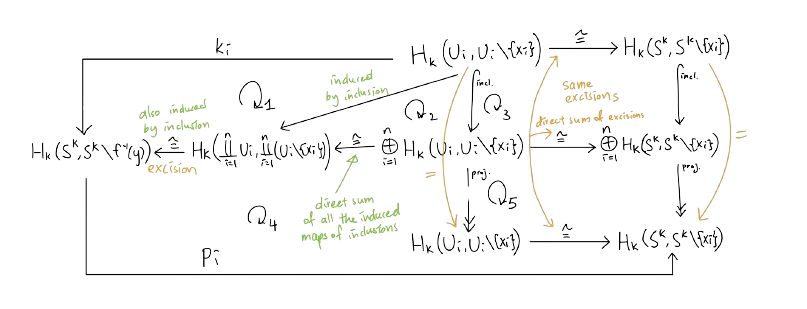
\includegraphics[scale = 0.5]{Image 3}
\end{center}

$k_i:H_k(U_i,U_i\setminus\{x_i\})\to H_k(S^k,S^k\setminus f^{-1}(y))$ is by definition of the composition of the obvious maps and so the upper left part of the diagram is commutativity. The upper middle part of the diagram commutes since both are induce by inclusions an direct sum of the induced maps of inclusions. The upper right and lower right part are commutative since they are induced by the same excisions and the direct sum of the very same excisions. Finally, $p_i:H_k(S^k,S^k\setminus f^{-1}(y))\to H_k(S^k,S^k\setminus\{x_i\})$ is defined to be the composition of the obvious maps and so the bottom left diagram is commutative by definition. \\~\\

All of the above shows that the upper left of the following diagram commutes: \\~\\
\adjustbox{scale=1.0,center}{\begin{tikzcd}
	& {H_k(U_i,U_i\setminus\{x_i\})} & {H_k(V,V\setminus\{y\})} \\
	{H_k(S^k,S^k\setminus\{x_i\})} & {H_k(S^k,S^k\setminus f^{-1}(y))} & {H_k(S^k,S^k\setminus\{y\})} \\
	& {H_k(S^k)} & {H_k(S^k)}
	\arrow["{f_\ast=\times\deg(f|_{x_i})}", from=1-2, to=1-3]
	\arrow["\cong"', from=1-2, to=2-1]
	\arrow["{k_i}"', from=1-2, to=2-2]
	\arrow["\cong", from=1-3, to=2-3]
	\arrow["{p_i}"', from=2-2, to=2-1]
	\arrow["{f_\ast}", from=2-2, to=2-3]
	\arrow["\cong", from=3-2, to=2-1]
	\arrow["{j_i}", from=3-2, to=2-2]
	\arrow["{f_\ast=\times\deg(f)}"', from=3-2, to=3-3]
	\arrow["\cong"', from=3-3, to=2-3]
\end{tikzcd}}\\~\\

The bottom left of this diagram is commutative because: 

\begin{center}
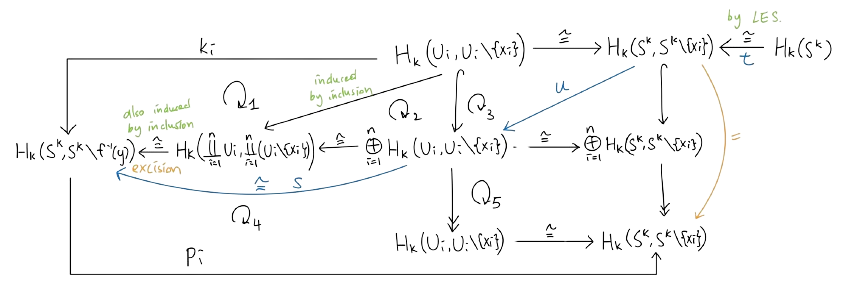
\includegraphics[scale = 0.5]{Image 4}
\end{center}

and $s\circ u\circ t$ is the map $j$. The isomorphism on the top right is obtained by excision. $k_i$ is induced by the inclusion $(S^k,S^k\setminus\{x_i\})\hookrightarrow(S^k,S^k\setminus f^{-1}(y))$ and then by the very same excision $$H_k(U_i,U_i\setminus\{x_i\})\cong H_k(S^k,S^k\setminus\{x_i\})$$ so that the top right square commutes. The isomorphism on the bottom right is given by the long exact sequence for relative homology. It is commutative by the naturality of long exact sequences for relative homology. \\~\\

By treating the middle term as $$H_k(S^k,S^k\setminus f^{-1}(y))$$ one can see that $k_i$ is just the inclusion into the direct summands. Similarly, using the first diagram of the proof we see that some part of $p_i$ is a projection of the direct summands. Commutativity of the third diagram shows that $p_i(j(1))=1$. Since $p_i$ is the projection from the direct summand, we must have that $p_i(0,\dots,0,1,0,\dots,0)=1$ which shows that $j(1)=(1,\dots,1)$. At the same time, $k_i$ is the inclusion into the direct summands thus $(1,\dots,1)=\sum_{i=1}^nk_i(1)$. Thus we conclude that $j(1)=\sum_{i=1}^nk_i(1)$. \\~\\

Now recall that $\deg(f)=f_\ast(1)$. By the lower part of the second diagram, we have that $$f_\ast(1)=f_\ast(j(1))=f_\ast\left(\sum_{i=1}^nk_i(1)\right)=\sum_{i=1}^nf_\ast(k_i(1))$$ By the top part of the second diagram, we conclude that $f_\ast(k_i(1))=\deg(f|_{x_i})$ for each $i$. Thus we have shown that $$\deg(f)=\sum_{i=1}^n\deg(f|_{x_i})$$ and so we are done. 
\end{proof}
\end{prp}

\subsection{Cellular Homology}
Singular homology is not often easy to calculate. A more combinatorial result comes from cellular homology, which actually gives the same result as singular homology. 

Recall that CW complexes and subcomplexes always forms good pairs. 

\begin{lmm}{}{} Let $X$ be a CW-complex with $n$-cells $\{D_\alpha^n\}$ for $n\geq 0$. Then $$H_k(X^n,X^{n-1})\cong\begin{cases}
\oplus_\alpha\Z\cdot\{D_\alpha^n\} & \text{ if } k=n\\
0 & \text{ otherwise }
\end{cases}$$ \tcbline
\begin{proof}
We have that $$H_k(X^n,X^{n-1})\cong\widetilde{H}_k(X^n/X^{n-1})\cong\widetilde{H}_k\left(\bigvee_\alpha D_\alpha^n/\partial D_\alpha^n\right)\cong\bigoplus_\alpha\widetilde{H}_k(D_\alpha^n/\partial D_\alpha^n)$$ and so we conclude. 
\end{proof}
\end{lmm}

In fact, one can explicitly describe the isomorphism as follows. For $D_\alpha^n$ in the $n$-skeleton in $X$, it is isomorphic to $\Delta^n$ an $n$-simplex. Thus we have a continuous map $$\Delta^n\cong D_\alpha^n\overset{\Phi_\alpha}{\longrightarrow}X$$ which is in fact a relative cycle for the pair $(X^n,X^{n-1})$. Its relative homology class then generates the copy of $\Z$ corresponding to $D_\alpha^n$. 

\begin{lmm}{}{} Let $X$ be a CW-complex. Then the following are true regarding the singular homology of $X$. 
\begin{itemize}
\item If $X$ is of dimension $k$ then $H_n(X)=0$ for all $n>k$. 
\item The map $H_n(X^m)\to H_n(X)$ induced by the inclusion $X^m\to X$ is an isomorphism if $n<m$ and surjective if $m=n$. 
\end{itemize} \tcbline
\begin{proof}
We proceed by induction. When $k=0$, it is obvious. Assume the statement is true for $k-1$. Consider the long exact sequence for relative homology: \\~\\
\adjustbox{scale=1.0,center}{\begin{tikzcd}
	\cdots & {H_{n+1}(X^k,X^{k-1})} & {H_n(X^{k-1})} & {H_n(X^k)} & {H_n(X^k,X^{k-1})} & \cdots
	\arrow[from=1-1, to=1-2]
	\arrow[from=1-2, to=1-3]
	\arrow[from=1-3, to=1-4]
	\arrow[from=1-4, to=1-5]
	\arrow[from=1-5, to=1-6]
\end{tikzcd}}\\~\\
By induction, the second term vanishes for $n>k$. By the previous lemma, the last term vanishes for $n>k$. Thus we obtain the required isomorphisms. \\~\\

Similarly, by the above long exact sequence, when $n<k-1$, both outer and terms vanish and the middle arrow becomes an isomorphism. For $n<k$, the last term vanishes and the middle arrow is a surjection. Thus for $n<m$, we have isomorphisms: \\~\\
\adjustbox{scale=1.0,center}{\begin{tikzcd}
	{H_n(X^m)} & {H_n(X^{m+1})} & {H_n(X^{m+2})} & \cdots
	\arrow[from=1-1, to=1-2]
	\arrow[from=1-2, to=1-3]
	\arrow[from=1-3, to=1-4]
\end{tikzcd}}\\~\\
By properties of the geometric realization, we must have that every compact subspace of $X$ must lie inside some $X^t$ for $t\in\N$. For any $\tau\in C_{n+1}(X)$, we thus have $\tau\in C_{n+1}(X^t)$ for some $t>n$. Hence $\tau$ maps to $0$ in $H_n(X^t)$ if $\tau$ is an $n$-cycle. Thus all these groups must be equal to $H_n(X)$. On the other hand, if $n=m$, then the first arrow $H_n(X^m)\to H_n(X^{m+1})$ is only surjective while the remaining ones are isomorphisms. Thus we are done. 
\end{proof}
\end{lmm}

Using the above lemma, we now have a spliced diagram : 
\\~\\
\adjustbox{scale=1.0,center}{\begin{tikzcd}
	&&& 0 \\
	0 && {H_n(X^{n+1})} \\
	& {H_n(X^n)} \\
	{H_{n+1}(X^{n+1},X^n)} && {H_n(X^n,X^{n-1})} && {H_{n-1}(X^{n-1},X^{n-2})} \\
	&&& {H_{n-1}(X^{n-1})} \\
	&& 0
	\arrow["\alpha", from=4-1, to=3-2]
	\arrow[from=3-2, to=2-3]
	\arrow[from=2-3, to=1-4]
	\arrow[from=2-1, to=3-2]
	\arrow["\beta", color={rgb,255:red,92;green,92;blue,214}, from=3-2, to=4-3]
	\arrow["\gamma", color={rgb,255:red,92;green,92;blue,214}, from=4-3, to=5-4]
	\arrow["{d_{n+1}}", color={rgb,255:red,214;green,92;blue,92}, from=4-1, to=4-3]
	\arrow["\delta", from=5-4, to=4-5]
	\arrow["{d_n}", color={rgb,255:red,214;green,92;blue,92}, from=4-3, to=4-5]
	\arrow[from=6-3, to=5-4]
\end{tikzcd}}\\~\\
where the diagonals come from the long exact sequence in the proof of the first part of lemma 7.4.3. The $d_n$ is then defined through the composition of the diagonal arrows. 

\begin{lmm}{}{} The composition $d_n\circ d_{n+1}$ is zero. \tcbline
\begin{proof}
The composition $d_n\circ d_{n+1}$ factors through the two blue arrows in the diagram. They are part of a long exact sequence and so their composition is $0$. 
\end{proof}
\end{lmm}

\begin{defn}{Cellular Chain Complex}{} Let $X$ be a CW-complex. Define the cellular chain complex $C_\bullet^\text{CW}(X)$ where $$C_n^{\text{CW}}(X)=H_n(X^n,X^{n-1})$$ together with differentials $d_n$ as defined above. Define the cellular homology groups of this chain complex to be $$H_n^\text{CW}(X)=H_n(C_\bullet^\text{CW}(X))$$
\end{defn}

\begin{lmm}{}{} For any CW-complex $X$, there are canonical isomorphisms $$H_n^\text{CW}(X)\cong H_n(X)$$ \tcbline
\begin{proof}
Since $\delta$ is injective, we have that $$\ker(d_n)=\ker(\gamma)=\im(\beta)$$ Also by lemma 7.3.2, we have that $H_n(X^{n+1})\cong H_n(X)$. This means that $$H_n(X)\cong\text{coker}(\alpha)\cong\frac{\im(\beta)}{\im(\beta\circ\alpha)}=\frac{\ker(d_n)}{\im(d_{n+1})}$$ where the second isomorphism comers from the fact that $\beta$ is injective. 
\end{proof}
\end{lmm}

Recall that a CW-complex $X$ is defined recursively through the use of attaching maps $\{\phi_\alpha:S_\alpha^{n-1}\to X^{n-1}|\alpha\in I_n\}$ for each $n$, such that $$X^n=\left(X^{n-1}\amalg\coprod_{\alpha\in I_n}D_\alpha^n\right)/\sim$$ where the equivalence relation is $x\sim\phi_\alpha(x)$ for all $x\in\partial D_\alpha^n$ (This is an amalgamated product over $\phi_\alpha(x)$). Notice that we have $$\frac{X^n}{X^{n-1}}\cong\bigvee_{\alpha\in I_n}\frac{D_\alpha^n}{\partial D_\alpha^n}=\bigvee_{\alpha\in I_n} S_\alpha^n$$ implies that there are canonical quotient maps obtain by collapsing all sphere other than one into a single point by an equivalence relation: \\~\\
\adjustbox{scale=1.0,center}{\begin{tikzcd}
	{\pi_\alpha:X^n} & {\frac{X^n}{X^{n-1}}\cong\bigvee_{\alpha\in I_n}S_\alpha^n} & {S_\alpha^n}
	\arrow[two heads, from=1-1, to=1-2]
	\arrow[two heads, from=1-2, to=1-3]
\end{tikzcd}} \\~\\

To compute the cellular homology of a CW complex, we already know that the chain complex has terms given by lemma 7.3.2. It remains to compute what the differentials look like. We will use this map in the following formula. 

\begin{thm}{Cellular Boundary Formula}{} Let $X$ be a CW-complex with attaching maps denoted $\phi_\alpha$, and $C_\bullet^\text{CW}(X)$ the cellular chain complex of $X$ with generators $\{[D_\alpha^n]|_{\alpha\in I_n}\}$ for each degree $n$. The boundary operator of the chain complex is given by the following formula: 
\begin{itemize}
\item In degree $n=1$, we have $$d_1\left([D_\alpha^1]\right)=[\phi_\alpha(1)]-[\phi_\alpha(0)]$$
\item In degrees $n>1$, we have $$d_n\left([D_\alpha^n]\right)=\sum_{\beta\in I_{n-1}}d_{\alpha\beta}\cdot[D_\beta^{n-1}]$$ where $$d_{\alpha\beta}=\deg\left(\Delta_{\alpha\beta}:S_\alpha^{n-1}\overset{\phi_\alpha}{\rightarrow}X^{n-1}\overset{\pi_\beta}{\rightarrow}S_\beta^{n-1}\right)$$ 
\end{itemize}
\end{thm}

On computation, one crucial fact to notice is that the map $\pi_\beta$ is a projection to the quotient topology. This means that after applying $\pi_\beta$, the map $$\Delta_{\alpha\beta}=\pi_\beta\circ\phi_\alpha:S_\alpha^{n-1}\to S_\beta^{n-1}$$ forgets about every boundary of the attached discs to $X^n$ other than the boundary of the disc $D_\beta^n$. Also notice that $\alpha\in I_n$ loops over all attaching maps and disks on the $n$th dimension, while $\beta\in I_{n-1}$ loops over that of the $n-1$ dimension. Notice that in the formula, $\beta$ is used to indicate the $S^{n-1}$ which are of dimension $n$. This makes sense because in $\pi_\beta$, there is a projection $X^{n-1}\to X^{n-1}/X^{n-2}$. $$\frac{X^{n-1}}{X^{n-2}}=\bigvee_{\beta\in I_{n-1}}\frac{D_\beta^{n-1}}{\partial D_\beta^{n-1}}$$ is then a wedge sum of all disks in dimension $n-1$ modulo boundary. \\~\\

We can now compute the singular homology of more complicated spaces such as the projective space. 

\begin{thm}{}{} Let $n\geq 1$. Then the real projective space $\R\Prj^n$ has the following homology groups: $$H_k(\R\Prj^n)=\begin{cases}
\Z & \text{ if }k=0\text{ and }k=n\text{ is odd}\\
\Z/2\Z & \text{ if } 0<k<n\text{ and }k\text{ is odd}\\
0 & \text{otherwise}
\end{cases}$$ \tcbline
\begin{proof}
Recall that the CW complex structure of $\R\Prj^n$ consists of one $k$-cell for each $0\leq k\leq n$. We have to determine the boundary operator. This is done by induction. \\~\\

The base case is obtained easily since $S^1\cong\R\Prj^1$. \\~\\

Suppose that the attaching maps are defined for all lower values of $k$. Recall that the attaching map of each $k$-cell is defined by the two-to-one map $f:S^{k-1}\to\R\Prj^{k-1}$. This forms the first part of the map $\Delta_{\alpha\beta}$ of the formula for the cellular boundary maps. To proceed, we quotient out the $X^{k-2}$ skeleton to obtain $$S^{k-1}\to\R\Prj^{k-1}\to\frac{\R\Prj^{k-1}}{\R\Prj^{k-2}}\cong S^{k-1}$$ We compute the degree of this map using local degrees. Since it is a two-to-one covering map, we concern ourselves with the north / south pole of $S^{k-1}$. Choose your favourite homeomorphism $D^{k-1}/\partial D^{k-1}\cong S^{k-1}$. Then the map $f:S^{k-1}\to\R\Prj^{k-1}$ is a local homeomorphism since it is a covering space. Thus the degree of the map is $\pm1$, fixed by the choice of the homeomorphism. This similar for the south pole. In fact, the map is identical to that of the local homeomorphism at the north pole and so the local homeomorphism is just the antipodal map composed with the local homeomorphism at the north pole. \\~\\

Denote $N$ and $S$ the north and south pole respectively. Since $\deg(f|_N)=\pm 1$ is fixed and the antipodal map has degree $(-1)^k$, we obtain $$\deg(f)=\deg(f|_N)+(-1)^n\deg(f|_N)=\begin{cases}
\pm2 & \text{ if } n \text{ is even}\\
0 & \text{ if } n \text{ is odd}
\end{cases}$$ Thus the cellular chain complex together with induction, is of the form \\~\\
\adjustbox{scale=1.0,center}{\begin{tikzcd}
	0 & \Z & \Z & \cdots & \Z & \Z & \Z & \Z & 0
	\arrow[from=1-1, to=1-2]
	\arrow["{d_k}", from=1-2, to=1-3]
	\arrow["{d_{k-1}}", from=1-3, to=1-4]
	\arrow["\pm2", from=1-4, to=1-5]
	\arrow["0", from=1-5, to=1-6]
	\arrow["{\pm 2}", from=1-6, to=1-7]
	\arrow["0", from=1-7, to=1-8]
	\arrow[from=1-8, to=1-9]
\end{tikzcd}}\\~\\
where $d_k=\pm2$ if $k$ is even and $d_k=0$ if $k$ is odd. It follows that $$\deg(f)=\deg(f|_N)+(-1)^n\deg(f|_N)=\begin{cases}
\pm2 & \text{ if } n \text{ is even}\\
0 & \text{ if } n \text{ is odd}
\end{cases}$$
\end{proof}
\end{thm}

\pagebreak
\section{Variants of Singular Homology}
\subsection{Unification of the Homology Theories}
We studied three different homology theories, namely the simplicial homology $H_\ast^{\Delta}$, singular homology $H_\ast$ and Cellular homology $H_\ast^{\text{CW}}$. We have seen that $H_\ast^{\text{CW}}(X)\cong H_n(X)$ for a CW-complex $X$. We can also show that singular homology does not give new information compared to simplicial homology. 

\begin{thm}{}{} Let $X$ be a topological space endowed with a $\Delta$-complex structure $(T,\abs{T}\cong X)$. The induced map $H_n^\Delta(X)\to H_n(X)$ by the map $s:\Delta^n\to X$ for each $s\in T^n$ is an isomorphism. \tcbline
\begin{proof}
Firstly, every $n$-simplex $s\in T$ induces a canonical continuous map $s:\Delta^n\to X$. This extends to a homomorphism $\Delta_n(T)\to C_n(X)$ and so to a chain map and descends to homology. \\~\\

Denote $T^k$ the $\Delta$-sets of simplices in $T$ of dimension at most $k$. Define $\Delta_\bullet(T^k,T^{k-1})=\Delta_\bullet(T^k)/\Delta_\bullet(T^{k-1})$ and accordingly, $H_n(\Delta_\bullet(T^k,T^{k-1}))$. Then the short exact sequence of chain complexes \\~\\
\adjustbox{scale=1,center}{\begin{tikzcd}
	0 & {\Delta_\bullet(T^{k-1})} & {\Delta_\bullet(T^k)} & {\Delta_\bullet(T^k,T^{k-1})} & 0
	\arrow[from=1-1, to=1-2]
	\arrow[from=1-2, to=1-3]
	\arrow[from=1-3, to=1-4]
	\arrow[from=1-4, to=1-5]
\end{tikzcd}} \\~\\
Together with the inclusion maps and by naturality in theorem 1.4.3, give the following: \\~\\
\adjustbox{scale=0.8,center}{\begin{tikzcd}
	\cdots & {H_{n+1}(T^k,T^{k-1})} & {H_n(T^{k-1})} & {H_n(T^{k-1})} & {H_n(T^k,T^{k-1})} & {H_{n-1}(T^{k-1})} & \cdots \\
	\cdots & {H_{n+1}(\abs{T^k},\abs{T^{k-1}})} & {H_n(\abs{T^{k-1}})} & {H_n(\abs{T^{k-1}})} & {H_n(\abs{T^k},\abs{T^{k-1}})} & {H_{n-1}(\abs{T^{k-1}})} & \cdots
	\arrow[from=1-1, to=1-2]
	\arrow[from=1-2, to=1-3]
	\arrow[from=1-2, to=2-2]
	\arrow[from=1-3, to=1-4]
	\arrow[from=1-3, to=2-3]
	\arrow[from=1-4, to=1-5]
	\arrow[from=1-4, to=2-4]
	\arrow[from=1-5, to=1-6]
	\arrow[from=1-5, to=2-5]
	\arrow[from=1-6, to=1-7]
	\arrow[from=1-6, to=2-6]
	\arrow[from=2-1, to=2-2]
	\arrow[from=2-2, to=2-3]
	\arrow[from=2-3, to=2-4]
	\arrow[from=2-4, to=2-5]
	\arrow[from=2-5, to=2-6]
	\arrow[from=2-6, to=2-7]
\end{tikzcd}} \\~\\
When $k=0$, $\abs{T^0}$ is a discrete topological space on the set $T^0$, and the map $H_n(T^0)\to H_n(\abs{T^0})$ is an isomorphism. By induction and the five lemma, the middle map is an isomorphism provided that the first and fourth maps are isomorphisms. \\~\\

Note that $\Delta_\bullet(T^{k-1})$ is a chain complex in degrees $k-1$, $k-2$, down to $0$. And $\Delta_\bullet(T^k)$ is the same chain complex with an additional term $\Z T_k$ in degree $k$. It follows that $\Delta_\bullet(T^k,T^{k-1})$ is the chain complex with $\Z T^k$ concentrated in degree $k$. In particular, we have that $$H_n(T^k,T^{k-1})=\begin{cases}
\Z T^k & \text{ if } n=k\\
0 & \text{ otherwise }
\end{cases}$$
By construction of the geometric realization, we have a homeomorphism $$\frac{\abs{T^k}}{\abs{T^{k-1}}}\cong\frac{\Delta^k\times T^k}{\partial\Delta^k\times T^k}\cong\bigvee_{T_k}\frac{\Delta^k}{\partial\Delta^k}$$ Using lemma 6.2.4 and lemma 6.2.5, we have that $$H_n(\abs{T^k},\abs{T^{k-1}})\cong\widetilde{H_n}(\abs{T^k}/\abs{T^{k-1}})\cong\begin{cases}
\Z T_k & \text{ if } n=k\\
0 & \text{ otherwisev }
\end{cases}$$
with generators corresponding to elements $s\in T^k$ via the relative cycles $s:\Delta^k\to\abs{T^k}$. It follows that an isomorphism occurs in the first and fourth position of the long exact sequence of relative homology groups. \\~\\

If $T=T^n$ for some $n\in\N$, we are done. \\~\\

Continuing the proof, let $z\in Z_n(T)$ be an $n$-cycle whose image in $H_n(\abs{T})$ vanishes. Then there exists $\tau\in C_{n+1}(\abs{T})$ with $\partial\tau=z$. Now since $\abs{T}$ is the geometric realization, we must have every compact subspace of $\abs{T}$ lying in some $\abs{T^k}$. Hence $\tau\in C_{n+1}(\abs{T^k})$ for some $k>n$. We deduce that $z$ maps to $0$ in $H_n(\abs{T^k})$. By the previous argument, we have taht $z=0\in H_n(T^k)=H_n(T)$. This shows injectivity of $H_n(T)\to H_n(\abs{T})$. \\~\\

Similarly, let $\sigma\in Z_n(T)$ be an $n$-cycle. We have seen that $\sigma\in Z_n(\abs{T^k})$ for some $k>n$ and by the argument above, $[\sigma]$ comes from $H_n(T^k)=H_n(T)$. This shows surjectivity of $H_n(T)\to H_n(\abs{T})$ and so we are done. 
\end{proof}
\end{thm}

We can finally show that simplicial homology is independent of the choice of $\Delta$-complex structure. 

\begin{crl}{}{} The simplicial homology $H_\bullet^\Delta(X)$ depends on $X$ only and not on the $\Delta$-complex structure. \tcbline
\begin{proof}
Indeed the geometric realization of any two $\Delta$-complex structure is isomorphic to the same singular homology group. 
\end{proof}
\end{crl}

\begin{crl}{}{} Suppose $X$ has a $\Delta$-complex structure with simplicies in dimension $\leq k$ only. Then $H_n(X)=0$ for all $n>k$. \tcbline
\begin{proof}
Direct since singular homology coincides with simplicial homology. 
\end{proof}
\end{crl}

\subsection{The Tensor Product Functor}
Let $R$ be a ring. Let $M,N$ be $R$-modules. Recall that we defined the tensor product of $M$ and $N$ via the universal property in Rings and Modules: The tensor product is an $R$-module $M\otimes_RN$ such that for any $R$-bilinear map $\varphi:M\times N\to L$ where $L$ is an $R$-module, there exists a unique map $\rho:M\otimes_RN\to L$ such that $$\varphi=\rho\circ u$$ where $u:M\times N\to M\otimes_RN$ is the map $(m,n)\mapsto(m\otimes n)$. \\

We specialize the case to where $R=\Z$. In this case, $M$ and $N$ are just abelian groups. 

\begin{defn}{The Tensor Product Functor}{} Let $G$ be an abelian group. Define the tensor product functor over $G$ to be the functor $$-\otimes G:\bold{Ab}\to\bold{Ab}$$ to consist of the following data. 
\begin{itemize}
\item For each abelian group $H\in\bold{Ab}$, the functor assigns the abelian group $H\otimes G$. 
\item For each group homomorphism $f:A\to B$, define the induced homomorphism $f\otimes G:A\otimes G\to B\otimes G$ by $$a\otimes g\mapsto f(a)\otimes g$$
\end{itemize}
\end{defn}

\begin{prp}{}{} Let $A,B,C,G$ be abelian groups. Let $f:A\to B$ and $g:B\to C$ be group homomorphisms. If $A\to B\to C\to 0$ is an exact sequence, then the sequence \\~\\
\adjustbox{scale=1,center}{\begin{tikzcd}
	{A\otimes G} & {B\otimes G} & {C\otimes G} & 0
	\arrow["{f\otimes G}", from=1-1, to=1-2]
	\arrow["{g\otimes G}", from=1-2, to=1-3]
	\arrow[from=1-3, to=1-4]
\end{tikzcd}} \\~\\
is exact. 
\end{prp}

\subsection{Homology with Coefficients}
We would now like to generalize singular homology so that the coefficients of the chain complex does not take values in $\Z$, but instead in an arbitrary group $G$. For this, we first modify the group of $n$-chains. 

\begin{defn}{Singular n-Chains with Coefficients in a Group}{} Let $X$ be a space. Let $G$ be an abelian group. Define the group of singular $n$-chains with coefficients in $G$ to be $$C_n(X;G)=C_n(X)\otimes G$$ Let $A\subseteq X$ be a subspace. Define the relative $n$-chains with coefficients in $G$ to be the group $$C_n(X,A;G)=\frac{C_n(X;G)}{C_n(A;G)}$$
\end{defn}

In particular, notice that the tensor product here just means that $C_n(X;G)$ is just copies of $G$, where the number of copies is precisely the number of singular $n$-simplexes in $X$. 

\begin{defn}{Boundary Operator}{} Let $X$ be a space. Let $G$ be an abelian group. Define the boundary operator of the singular chain complex with coefficients in $G$ to be $$\partial_G=\partial_n\otimes 1_G:C_n(X;G)\to C_{n-1}(X;G)$$ defined by $\sigma\otimes g\mapsto\partial_n(\sigma)\otimes g$ and then extended linearly. 
\end{defn}

\begin{lmm}{}{} Let $X$ be a space. Let $G$ be an abelian group. Then $\partial_G\circ\partial_G=0$. Moreover, the groups $C_n(X;G)$ together with the boundary operator $\partial_G$ is a chain complex. 
\end{lmm}

\begin{defn}{Singular Homology with Coefficients}{} Let $X$ be a space. Let $G$ be an abelian group. Define the singular homology groups of $X$ to be the homology groups of the chain complex $(C_\bullet(X;G),\partial_G)$. This means that $$H_n(X;G)=\frac{\ker(\partial_G:C_n(X;G)\to C_{n-1}(X;G))}{\im(\partial_G:C_{n+1}(X;G)\to C_n(X;G))}=H_n(C_\bullet(X;G))$$ for $n\in\N$. 
\end{defn}

A natural question would be to ask whether there is a relation between homology with integer coefficients $H_n(X)$ and homology with arbitrary coefficients $H_n(X;G)$. Namely, the chain complex for singular homology with coefficients simply replaces the integral coefficients of the original singular chain complex via the tensor product. Is there a natural association between $H_n(X)\otimes G$ and $H_n(X;G)$? \\~\\

The answer is yes, but it is not an isomorphism. Moreover, there is a way to measure the failure of the isomorphism in a natural and functorial way. This will be delayed to later sections. 

\subsection{Axioms of Homology}
\begin{defn}{Generalized Homology Theory for CW Pairs}{} A Generalized Homology Theory is a collection of functors and natural transformations $$h_n:\bold{CW}^2\to\bold{Ab}\;\;\;\;\text{ and }\;\;\;\;\delta_n:h_n\Rightarrow h_n\circ F$$ where $F(X,Y)=(Y,\emptyset)$, for each $n\in\N$, such that the following are true. 
\begin{itemize}
\item Homotopy Invariance: If $f\simeq g:(X,A)\to(Y,B)$ then $$h_n(f)=h_n(g):h_n(X,A)\to h_n(Y,B)$$
\item Exactness: There exists an exact sequence \\~\\
\adjustbox{scale=0.98,center}{\begin{tikzcd}
	\cdots & {h_{n+1}(X,A)} & {h_n(A,\emptyset)} & {h_n(X,\emptyset)} & {h_n(X,A)} & {h_{n-1}(A,\emptyset)} & \cdots
	\arrow[from=1-1, to=1-2]
	\arrow["{\delta_{n+1}}", from=1-2, to=1-3]
	\arrow["h_n(i)", from=1-3, to=1-4]
	\arrow["h_n(j)", from=1-4, to=1-5]
	\arrow["{\delta_n}", from=1-5, to=1-6]
	\arrow[from=1-6, to=1-7]
\end{tikzcd}}\\~\\
where $i:(A,\emptyset)\to(X,\emptyset)$ and $j:(X,\emptyset)\to(X,A)$ are inclusions. 
\item Excision: If $\overline{E}\subseteq A^\circ\subseteq X$, then there is an isomorphism $$h_n(X\setminus E,A\setminus E)\cong h_n(X,A)$$ induced by the inclusion map. 
\end{itemize}
\end{defn}

The homotopy invariance axiom means that homology descends to a functor $\bold{HoCW}^2\to\bold{Ab}$. Therefore some authors write the axiom implicit in the definition of the functors $h_n$, and then saying that a homology theory consists of functors $h_n:\bold{HoCW}\to\bold{Ab}$ instead. 

\begin{lmm}{}{} The excision axiom is equivalent to saying that $X=A^\circ\cup B^\circ$ with inclusion map $\iota:(B,A\cap B)\to (X,A)$ implies $h_n(\iota):h_n(B,A\cap B)\to h_n(X,A)$ is an isomorphism. 
\end{lmm}

\begin{defn}{Additive Homology Theory}{} Let $h_n:\bold{CW}^2\to\bold{Ab}$ be a generalized homology theory. We say that $h_n$ is additive if the following axiom is satisfied. 
\begin{itemize}
\item Additivity: If $(X,A)=\coprod_{i\in I}(X_i,A_i)$, then the direct sum of the inclusion maps $$\bigoplus_{i\in I}h_n(X_i,A_i)\cong h_n(X,A)$$ is an isomorphism
\end{itemize}
\end{defn}

We mention for once and for all that the additivity axiom is required only when the CW complexes are non-finite. In particular, in order for the homology theory to be meaningful, we must restrict the underlying category of spaces to be finite CW complexes if one drops the additivity axiom. \\~\\

\begin{defn}{Generalized Homology Theory for Spaces}{} A Generalized Homology Theory is a collection of functors $$h_n:\bold{Top}^2\to\bold{Ab}\;\;\;\;\;\;\;\text{ and }\;\;\;\;\;\;\;\delta_n:h_n\circ F\Rightarrow h_{n-1}$$ where $F(X,Y)=(Y,\emptyset)$, for each $n\in\N$, satisfying the first four axioms together with the following. 
\begin{itemize}
\item Weak Equivalence: If $f:(X,A)\to(Y,B)$ is a weak equivalence, then $$f_\ast:h_n(X,A)\to h_n(Y,B)$$ is an isomorphism. 
\end{itemize}
\end{defn}

By adding on the axiom of weak equivalence and the fact that every space admits a weak equivalence to a CW complex, we can see that the two theories are the same. 

\begin{thm}{}{} Any generalized homology theory on $\bold{Top}^2$ determines and is determined by a generalized homology theory on $\bold{CW}^2$.
\end{thm}

\begin{defn}{Ordinary Homology Theory}{} Let $G$ be an abelian group. If a generalized homology theory $(h_n,\delta_n)$ in addition satisfies 
\begin{itemize}
\item Dimension: $$h_n(\ast)=\begin{cases}
G & \text{ if } n=0\\
0 & \text{ otherwise }
\end{cases}$$
\end{itemize}
Then $h_n$ is called an ordinary homology theory. 
\end{defn}

\begin{thm}{Eilenberg-Steenrod Uniqueness Theorem}{} Let $T:(h_n,\delta_n)\to(h_n',\delta_n')$ be a natural transformation of generalized homology theories defined on $\bold{CW}^2$ such that $h_n(\ast)\cong h_n'(\ast)$, then $T$ is a natural isomorphism $$(h_n,\delta_n)\cong(h_n',\delta_n')$$
\end{thm}

\pagebreak
\section{Algebra of Cochain Complexes}
\subsection{Cochain Complexes}
\begin{defn}{Cochain Complexes}{} Let $R$ be a ring. A cochain complex $(C^\bullet,\partial^\bullet)$ over $R$ is a family of $R$-modules $C^n$ for $n\in\Z$ and $R$-module homomorphisms $\delta^n:C^{n-1}\to C^n$ such that $\delta^{n+1}\circ\delta^n=0$ for all $n$. In other words, we have the diagram: \\~\\
\adjustbox{scale=1.0,center}{\begin{tikzcd}
\cdots & C^{n+1}\arrow[l] & C^n\arrow[l, "\delta^{n+1}"'] & C^{n-1}\arrow[l, "\delta^n"'] & \cdots\arrow[l]
\end{tikzcd}}
\end{defn}

Notice that algebraically, there is no difference between a chain complex and a cochain complex, other than the fact that the boundary maps run in the other direction. For $(C_\bullet,\partial_\bullet)$ a chain complex, we can form a cochain complex by setting $C^n=C_{-n}$ and then using the same boundary maps. 

\begin{defn}{Category of Cochain Complexes}{} Let $R$ be a ring. Define the category of cochain complexes $$\bold{CCh}(R)$$ to consist of the following data. 
\begin{itemize}
\item The objects are the cochain complexes over $R$
\item The morphisms are the chain maps
\item Composition is given by the composition of maps on all levels of the chain map. 
\end{itemize}
\end{defn}

Because cochain complexes is the same data as a chain complex, we can also define homology groups for cochain complexes. We call them the cohomology groups of the cochain complex. 

\begin{defn}{Cohomology Groups}{} Let $R$ be a ring. Let $(C^\bullet,\partial^\bullet)$ be a cochain complex over $R$. Define the $n$th cohomology group of the cochain complex to be $$H^n(C^\bullet,\partial^\bullet)=\frac{\ker(\partial^{n+1}:C^n\to C^{n+1})}{\im(\partial^n:C^{n-1}\to C^n)}=H_n(C^\bullet,\partial^\bullet)$$ for $n\in\N$. 
\end{defn}

The construction of cohomology groups are functorial because the homology groups of a chain complex also are. 

\begin{defn}{The Cohomology Functor}{} Let $R$ be a ring. Let $n\in\N$. Define the $n$th cohomology functor to be the functor $$H^n:\bold{CCh}(R)\to\bold{Ab}$$ to consist of the following data. 
\begin{itemize}
\item For each cochain complex $(C^\bullet,\delta^\bullet)$ over $R$, define $H^n(C^\bullet,\delta^\bullet)$ to be the $n$th cohomology group of the cochain complex. 
\item For each chain map $f^\bullet:(C^\bullet,\delta^\bullet)\to(D^\bullet,\delta^\bullet)$, the induced map $$f^\ast:H^n(C^\bullet,\delta^\bullet)\to H^n(C^\bullet,\delta^\bullet)$$ is defined by $[z]\mapsto[f^n(z)]$. 
\end{itemize}
\end{defn}

Notice that obtaining cohomology from chain complexes is covariant. 

\subsection{Producing a Cochain Complex from a Chain Complex}
Let $R$ be a ring. Let $M,N$ be $R$-modules. Recall that $\Hom_R(M,N)$ is only an abelian group, and at most a $Z(R)$-ring in general. However, when $R$ is commutative, $\Hom_R(M,N)$ becomes an $R$-module. Here we treat the more general case and consider the case when $R$ is a general ring. 

\begin{defn}{Dualization of a Chain Complex}{} Let $R$ be a ring. Let $(C_\bullet,\partial_\bullet)$ be a chain complex. Let $M$ be an $R$-module. For each $R$-module $C_n$, define the associated cochain group to be $$C^n=\Hom_R(C_n,M)$$ Also define the coboundary map $\delta^n=\partial_n^\ast:C^{n-1}\to C^n$ by $$\delta^n(\phi)(\alpha)=\psi(\partial_{n+1}(\alpha))$$
\end{defn}

\begin{lmm}{}{} Let $(C_\bullet,\partial_\bullet)$ be a chain complex and let $C^\bullet$ and $\delta^\bullet$ be the associated cochain groups and coboundary maps respectively. Then $$\delta^n\circ\delta^{n-1}=0$$ for all $n$ such that $(C^\bullet,\delta^\bullet)$ is a cochain complex. 
\end{lmm}

\begin{defn}{The Hom Functor on Chain Complexes}{} Let $R$ be a ring. Let $M$ be an $R$-module. Define the (contravariant) Hom functor on chain complexes to be the functor $$\Hom(-;M):\bold{Ch}(R)\to\bold{CCh}(\Z)$$ consisting of the following data. 
\begin{itemize}
\item For $(C_\bullet,\partial_\bullet)$ a chain complex, define a cochain complex by $C^n=\Hom(C_n;G)$ and coboundary map by $\delta_n=\partial_n^\ast$
\item For a chain map $f_\bullet:(C_\bullet,\delta_\bullet)\to(D_\bullet,\delta_\bullet)$, define a chain map $f^\ast:D^n\to C^n$ by $\varphi\mapsto\varphi\circ f$. 
\end{itemize}
\end{defn}

If $R$ is commutative, we can upgrade the structure of the Hom sets to get a Hom functor of the form $$\Hom(-;M):\bold{Ch}(R)\to\bold{Ch}(R)$$

\begin{prp}{}{} Let $C_\bullet,D_\bullet,E_\bullet\in\bold{Ch}(\Z)$ be chain complexes such that the short exact sequence \\~\\
\adjustbox{scale=1.0,center}{\begin{tikzcd}
	0 & {C_\bullet} & {D_\bullet} & {E_\bullet} & 0
	\arrow[from=1-1, to=1-2]
	\arrow["f", from=1-2, to=1-3]
	\arrow["g", from=1-3, to=1-4]
	\arrow[from=1-4, to=1-5]
\end{tikzcd}}\\~\\
of chain complexes is degree wise split (this means that $D_n\cong C_n\oplus E_n$ for all $n\in\N$). Then the dual of the chain complex \\~\\
\adjustbox{scale=1.0,center}{\begin{tikzcd}
	0 & {E^\bullet} & {D^\bullet} & {C^\bullet} & 0
	\arrow[from=1-1, to=1-2]
	\arrow["{g^\ast}", from=1-2, to=1-3]
	\arrow["{f^\ast}", from=1-3, to=1-4]
	\arrow[from=1-4, to=1-5]
\end{tikzcd}}\\~\\
is also a short exact sequence of chain complexes. 
\end{prp}

We have now defined a series of functors. We also recap on the material in section 1. 
\begin{itemize}
\item We have defined the homology functor of chain complexes $$H_n:\bold{Ch}(\Z)\to\bold{Ab}$$ for each $n\in\N$. 
\item Using the very same functor, but thinking about cochain complexes as chain complexes in the wrong direction, we have also defined the cohomology functor of cochain complexes $$H^n:\bold{CCh}(\Z)\to\bold{Ab}$$ for each $n\in\N$. 
\item Specializing to the case $R=\Z$, we have a functorial method of dualizing chain complexes into cochain complexes by the functor $$\Hom(-;A):\bold{Ch}(\Z)\to\bold{CCh}(\Z)$$ for any abelian group $A$. 
\end{itemize}

\pagebreak
\section{The Choice of Coefficients in Singular (Co)Homology}
\subsection{Free Resolutions}
\begin{defn}{Free Resolutions}{} Let $H$ be a group. An exact sequence of the form \\~\\
\adjustbox{scale=1.0,center}{\begin{tikzcd}
\cdots\arrow[r] & F_1\arrow[r] & F_0\arrow[r] & H\arrow[r] & 0
\end{tikzcd}}\\~\\
is said to be a free resolution of $H$ if $F_n$ is a free group for $n\in\N$. 
\end{defn}

\begin{prp}{}{} Let $G$ and $H$ be abelian groups. Let $f:G\to H$ be a homomorphism. Suppose that there are free resolutions \\~\\
\adjustbox{scale=1.0,center}{\begin{tikzcd}
	\cdots & {F_1} & {F_0} & G & 0 \\
	\cdots & {E_1} & {E_0} & H & 0
	\arrow[from=1-1, to=1-2]
	\arrow["p_1", from=1-2, to=1-3]
	\arrow["p_0", from=1-3, to=1-4]
	\arrow[from=1-4, to=1-5]
	\arrow["f", from=1-4, to=2-4]
	\arrow[from=2-1, to=2-2]
	\arrow["q_1", from=2-2, to=2-3]
	\arrow["q_0", from=2-3, to=2-4]
	\arrow[from=2-4, to=2-5]
\end{tikzcd}}\\~\\
for $G$ and $H$ respectively. Let $f:G\to H$ be a group homomorphism. Then there exists a chain map extending $f$ such that the following diagram commutes: \\~\\
\adjustbox{scale=1.0,center}{\begin{tikzcd}
	\cdots & {F_1} & {F_0} & G & 0 \\
	\cdots & {E_1} & {E_0} & H & 0
	\arrow[from=1-1, to=1-2]
	\arrow["p_1", from=1-2, to=1-3]
	\arrow["p_0", from=1-3, to=1-4]
	\arrow["{f_1}", from=1-2, to=2-2]
	\arrow["{f_0}", from=1-3, to=2-3]
	\arrow[from=1-4, to=1-5]
	\arrow["f", from=1-4, to=2-4]
	\arrow[from=2-1, to=2-2]
	\arrow["q_1", from=2-2, to=2-3]
	\arrow["q_0", from=2-3, to=2-4]
	\arrow[from=2-4, to=2-5]
\end{tikzcd}}\\~\\
Moreover, any two such chain maps are homotopic. \tcbline
\begin{proof}
We will define the maps $f_n:F_n\to E_n$ for $n\in\N$ inductively. Since each $F_i$ is free, we only need to define the map on the basis elements of $F_i$. Consider the base case $n=0$. Since $E_0\to H$ is surjective, for any $x\in F_0$, there exists $x'\in E_0$ such that $q_0(x')=f(p_0(x))$. Define the map $f_0:F_0\to E_0$ by sending any basis element $x$ of $F_0$ to such an $x'$. (The $x'$ here may not be unique but we will show that any choice here leads to homotopic maps). \\~\\

Now suppose that $f_{k-1}:F_{k-1}\to E_{k-1}$ is defined such that $q_{k-1}\circ f_{k-1}=f_{k-2}\circ p_{k-1}$. Let $y\in F_k$. Then $f_{k-1}(p_k(y))\in E_{k-1}$. Now we have $$q_{k-1}((f_{k-1}\circ p_k)(y))=(f_{k-2}\circ p_{k-1}\circ p_k)(y)=f_{k-2}(0)=0$$ which shows that $(f_{k-1}\circ p_{k-1})(y)\in\ker(q_{k-1})=\im(q_k)$. But this means that there exists $y'\in E_k$ such that $q_k(y')=(f_{k-1}\circ p_k)(y)$. Therefore we define $f_k:F_k\to E_k$ by sending any basis element $y$ of $F_k$ to the defined $y'$. (Again the choice does not matter because any two choices of maps are homotopic). \\~\\

For uniqueness up to homotopy, suppose that $(g_k)_{k\in\N}$ is another such extension. Now consider the map $\alpha_k=f_k-g_k:F_k\to E_k$. The proof will be complete if the new chain map $\alpha$ is homotopic to the $0$ map. Because then $\alpha\simeq 0$ implies $f-g\simeq 0$ which implies $f\simeq g$. To show the null-homotopy, we need to define chain homotopies $\lambda_k:F_k\to E_{k+1}$ such that $\alpha_k=q_{k+1}\circ\lambda_k+\lambda_{k-1}\circ p_k$. We proceed by induction. \\~\\

For the map $\lambda_{-1}:G\to E_0$ we define it to be the $0$ map. When $k=0$, define $\lambda_0:F_0\to E_1$ as follows. Let $x\in F_0$ be a basis element. Then $f(p_0(x))=0$ and $g(p_0(x))=0$. Now we have that $$q_0(\alpha_0(x))=q_0((f_0-g_0)(x))=q_0(f_0(x))-q_0(g_0(x))=f(p_0(x))-g(p_0(x))=(f-g)(p_0(x))=0$$ because $f$ and $g$ are the same map. This means that $\alpha_0(x)\in\ker(q_0)=\im(q_1)$. Thus there exists $x'\in E_1$ such that $q_1(x')=\alpha_0(x)$. Therefore we define $\lambda_0:F_0\to E_1$ by sending any basis element $x\in F_0$ to the constructed $x'\in E_1$. But this is exactly what we want because it satisfies the chain condition: $$q_1(\lambda_0(x))+\lambda_{-1}(p_0(x))=q_0(\lambda_0(x))=q_1(x')=\alpha_0(x)$$~\\

Inductively, suppose that $\lambda_{k-1}:F_{k-1}\to E_k$ is already defined such that the chain homotopy condition is satisfied. Let $x\in F_k$ be a basis element. Then notice that 
\begin{align*}
q_k((\alpha_k-\lambda_{k-1}\circ p_k)(x))&=(q_k\circ\alpha_k)(x)-(q_k\circ\lambda_k\circ p_k)(x)\\
&=(q_k\circ f_k-q_k\circ g_k)(x)-(q_k\circ\lambda_k\circ p_k)(x)\\
&=(f_{k-1}\circ p_k-g_{k-1}\circ p_k)(x)-(q_k\circ\lambda_k\circ p_k)(x)\\
&=(f_{k-1}-g_{k-1})(p_k(x))-(q_k\circ\lambda_k\circ p_k)(x)\\
&=(\alpha_{k-1}\circ p_k)(x)-(q_k\circ\lambda_k\circ p_k)(x)\\
&=(\alpha_{k-1}-q_k\circ\lambda_k)(p_k(x))\\
&=(\lambda_{k-2}\circ p_{k-1}\circ p_k)(x)\tag{Chain Homotopy Condition}\\
&=\lambda_{k-2}(0)\\
&=0
\end{align*}
This shows that $(\alpha_k-\lambda_{k-1}\circ p_k)(x)\in\ker(q_k)=\im(q_{k+1})$, and hence there exists $x'\in E_{k+1}$ such that $q_{k+1}(x')=(\alpha_k-\lambda_{k-1}\circ p_k)(x)$. So we define $\lambda_k:F_k\to E_{k+1}$ by sending any basis element $x\in F_k$ to the constructed $x'\in E_{k+1}$. But this is exactly what we want because it satisfies the chain condition: 
\begin{align*}
(q_{k+1}\circ\lambda_k)(x)+(\lambda_{k-1}\circ p_k)(x)&=q_{k+1}(x')+(\lambda_{k-1}\circ p_k)(x)\\
&=(\alpha_k-\lambda_{k-1}\circ p_k)(x)+(\lambda_{k-1}\circ p_k)(x)\\
&=\alpha_k(x)
\end{align*}
And so we conclude. 
\end{proof}
\end{prp}

It follows from the algebra of chain complexes that any two such homotopic chain maps of free resolutions induce isomorphic cohomology groups. 

\begin{lmm}{}{} Every free resolution of an abelian group $H$ is of the form \\~\\
\adjustbox{scale=1.1,center}{\begin{tikzcd}
0\arrow[r] & F_1\arrow[r] & F_0\arrow[r, "h"] & H\arrow[r] & 0
\end{tikzcd}}\\~\\
where $F_0$ and $F_1$ is determined as follows. 
\begin{itemize}
\item Choose a set of generators $A$ of $H$. Define $F_0=\langle A\rangle$ and define the map $f_0:F_0\to H$ by sending basis elements to generators. 
\item $F_1=\ker(f_0)$ and $f_1:F_1\to F_0$ is the inclusion. 
\end{itemize} \tcbline
\begin{proof}
We want to show that using the above data to construct the free resolution gives an exact sequence. Clearly since $f_1:F_1\to F_0$ is the inclusion, it is injective. Also, $h$ is defined to be surjective. It remains to show that $\im(f_1)=\ker(f_0)$. But by definition, $f_1$ is the inclusion map of $\ker(f_0)$ to $F_1$ hence $\im(f_1)=\ker(f_0)$. 
\end{proof}
\end{lmm}

\subsection{Universal Coefficient Theorem for Cohomology}
\begin{defn}{Ext Group}{} Let $G,H$ be an abelian group. Choose a free resolution $F_\bullet$ of $H$: \\~\\
\adjustbox{scale=1.0,center}{\begin{tikzcd}
0\arrow[r] & F_1\arrow[r] & F_0\arrow[r] & H\arrow[r] & 0
\end{tikzcd}}\\~\\
Define the ext group of $H$ with coefficients in $G$ to be the first cohomology group of the cochain complex with coefficients in $G$ associated to this chain complex: $$\text{Ext}(H,G)=\text{Ext}_\Z^1(H,G)=\frac{\Hom(F_1,G)}{\im(\Hom(F_0,G)\to\Hom(F_1,G))}=H^1(\Hom(F_\bullet;G))$$
\end{defn}

The Ext group is well defined because of any choice of free resolution are chain chomotopic by a unique chain map. Moreover, chain homotopic maps induce isomorphisms on homology. This isomorphism is moreover canonical because the chain homotopy is given by a unique chain map. \\

A kind note: This is not the most general definition of an ext group. There are a few ways to advance this definition into the general one (as in Homological Algebra). Notice that every abelian group is a $\Z$-module. So we can define Ext groups depending on the underlying ring / module structure. For instance, if $M,N$ are $R$-modules, then there is a notion $\text{Ext}_R^1(M,N)$. In this case we no longer consider only free resolutions because free here refers to every abelian group is a $\Z$-module. Moreover, not every such resolution will only consist of two elements just as lmm 11.1.3. \\~\\

This leads to the second way of extending it. One can consider not using free groups for the resolution, and instead in the setting of $R$-modules, consider using projective / injective modules (again in Homological Algebra). \\~\\

For us, we are only considering abelian groups which are $\Z$-modules. Be wary of this assumption throughout the entire section. 

\begin{prp}{}{} Let $G,H,K$ be abelian groups. Then the following are true regarding the Ext group. 
\begin{itemize}
\item $\text{Ext}(H\oplus K,G)\cong\text{Ext}(H,G)\oplus\text{Ext}(K,G)$
\item $\text{Ext}(H,G)=0$ if $H$ is a free group. 
\item $\text{Ext}(\Z/n\Z,G)\cong G/nG$
\item $\text{Ext}(G,\Q)=0$
\end{itemize} \tcbline
\begin{proof}~\\
\begin{itemize}
\item Let $A_\bullet$ be a free resolution of $H$. Let $B_\bullet$ be a free resolution of $K$. I claim that \\~\\
\adjustbox{scale=0.85,center}{\begin{tikzcd}
	0 & {A_1\oplus B_1} & {A_0\oplus B_0} & {H\oplus K} & 0
	\arrow[from=1-1, to=1-2]
	\arrow[from=1-2, to=1-3]
	\arrow[from=1-3, to=1-4]
	\arrow[from=1-4, to=1-5]
\end{tikzcd}}\\~\\
with the direct sum of the obvious maps is a free resolution of $H\oplus K$. But this is obvious because the direct sum of free groups is again a free group. Now we have that 
\begin{align*}
\text{Ext}(H\oplus K)&=\frac{\Hom(H\oplus K,G)}{\im(A_0\oplus B_0\to H\oplus K)}\\
&\cong\frac{\Hom(H,G)\oplus\Hom(K,G)}{\im(A_0\to H_0)\oplus\im(B_0\to K_0)}\\
&\cong\frac{\Hom(H,G)}{\im(A_0\to H_0)}\oplus\frac{\Hom(K,G)}{\im(B_0\to K_0)}\\
&=\text{Ext}(H,G)\oplus\text{Ext}(K,G)
\end{align*}
\item If $H$ is already a free group, then $0\to H\to H\to 0$ with the identity map is a free resolution of $H$. Then by the definition of $\text{Ext}$ groups we conclude that $\text{Ext}(H,G)=0$
\end{itemize}
\end{proof}
\end{prp}

\begin{eg}{}{} The following are some computations of the Ext group. 
\begin{itemize}
\item $\text{Ext}(\Z/2\Z,\Z/3\Z)\cong\Z/6\Z$
\item $\text{Ext}(\Z/6\Z,\Z/2\Z)$
\item $\text{Ext}(\Z/4\Z,\Z/8\Z)$
\end{itemize}
\end{eg}

\begin{prp}{}{} Let $A,B,G$ be abelian groups. Let $f:A\to B$ be a group homomorphism. Define the induced map $$f^\ast:\text{Ext}(B,G)\to\text{Ext}(A,G)$$ as follows. Then $f^\ast$ is a group homomorphism. Moreover, the following are true. 
\begin{itemize}
\item Let $C$ be an abelian group and let $g:B\to C$ be a homomorphism. Then $$(g\circ f)^\ast=f^\ast\circ g^\ast$$ 
\item We have that $$\text{id}^\ast=\text{id}_{\text{Ext}(A,G)}:\text{Ext}(A,G)\to\text{Ext}(A,G)$$
\end{itemize}
\end{prp}

We conclude that $\text{Ext}$ is a functor of the first variable. It is also a functor of the second variable but we will not prove it. 

\begin{prp}{}{} Let $0\to A\to B\to C\to 0$ be a short exact sequence of abelian groups. Then there is a six term exact sequence: \\~\\
\adjustbox{scale=0.85,center}{\begin{tikzcd}
	0 & {\Hom(C,G)} & {\Hom(B,G)} & {\Hom(A,G)} & {\text{Ext}(C,G)} & {\text{Ext}(B,G)} & {\text{Ext}(A,G)} & 0
	\arrow[from=1-1, to=1-2]
	\arrow[from=1-2, to=1-3]
	\arrow[from=1-3, to=1-4]
	\arrow[from=1-4, to=1-5]
	\arrow[from=1-5, to=1-6]
	\arrow[from=1-6, to=1-7]
	\arrow[from=1-7, to=1-8]
\end{tikzcd}}
\end{prp}

The point of the Ext group is that it forms an error term to measure how far away is the cohomology of the dualized chain complex from the homology of the chain complex. 

\begin{thm}{Universal Coefficient Theorem for Cohomology}{} Let $(C_\bullet,\partial_\bullet)$ be a chain complex of free abelian groups. Let $G$ be an abelian group. Then there exists a natural map $h:H^n(C_\bullet;G)\to\Hom(H_n(C_\bullet;G))$ such that $$\text{Ext}(H_{n-1}(C_\bullet),G)\cong\ker(h)$$ and a split exact sequence (that is not natural) of the form \\~\\
\adjustbox{scale=1.0,center}{\begin{tikzcd}
0\arrow[r] & \text{Ext}(H_{n-1}(C_\bullet),G)\arrow[r] & H^n(C_\bullet;G)\arrow[r, "h"] & \Hom(H_n(C_\bullet),G)\arrow[r] & 0
\end{tikzcd}}\\~\\
for any $n\in\N$. In particular, split exactness implies that there is an isomorphism $$H^n(C_\bullet;G)\cong\text{Ext}(H_{n-1}(C_\bullet),G)\oplus\Hom(H_n(C_\bullet),G)$$ for any $n\in\N$. \tcbline
\begin{proof}
Define $h$ as follows. Let $[\alpha]\in H^n(C_\bullet,G)$. Then $\alpha\in\ker(\delta:C^n\to C^{n+1})\leq C^n$. Rephrasing shows that $\alpha$ is a homomorphism $C_n\to G$. We can then restrict $\alpha$ to the subgroup $Z_n\leq C_n$. I claim that $\alpha|_{Z_n}$ descends to a map in homology. This means that there exists a unique map $\overline{\alpha|_{Z_n}}:H_n(C_\bullet)\to G$ such that the following diagram commutes \\~\\
\adjustbox{scale=1.0,center}{\begin{tikzcd}
	{Z_n} & {\frac{Z_n}{B_n}=H_n(C_\bullet)} \\
	& G
	\arrow["p", from=1-1, to=1-2]
	\arrow["{\alpha|_{Z_n}}"', from=1-1, to=2-2]
	\arrow["{\exists!\overline{\alpha|_{Z_n}}}", dashed, from=1-2, to=2-2]
\end{tikzcd}}\\~\\
where $p$ is the projection map. But this is true since for any $x\in C_{n+1}$ such that $\partial x\in B_n$, we have that $$\alpha(\partial(x))=\delta(\alpha(x))=0$$ where the last equality comes from the fact that $\alpha\in\ker(\delta:C^n\to C^{n+1})$. By the universal property of quotients, $\overline{\alpha|_{Z_n}}$ exists and is unique. We finally define $h$ by $$h([\alpha])=\left[\overline{\alpha|_{Z_n}}\right]$$~\\

I claim that this is well defined. This means to show that if $[\alpha]=[\beta]$ then $h([\alpha])=h([\beta])$. So suppose that $[\alpha]=[\beta]$, then $\alpha+y=\beta$ for some $y\in B^n=\im(\delta:C^{n-1}\to C^n)$. This means that there exists $\overline{y}\in C^{n-1}$ such that $\delta(\overline{y})=y$. Now we have that 
\begin{align*}
h([\beta])&=\left[\overline{\beta|_{Z_n}}\right]\\
&=\left[\overline{(\alpha+y)|_{Z_n}}\right]\\
&=\left[\overline{(\alpha+\delta(\overline{y}))|_{Z_n}}\right]\\
&=\left[\overline{(\alpha+\overline{y}\circ\partial)|_{Z_n}}\right]\\
&=\left[\overline{(\alpha)|_{Z_n}}\right]\tag{$\partial$ restricted to $Z_n$ is just $0$}\\
&=h([\alpha])
\end{align*}
Thus $h$ is well defined. \\~\\

We now show that $h$ is split surjective. Define a map $v:\Hom(H_n(C_\bullet,G))\to H^n(C_\bullet,G)$ as follows. Let $\theta\in\Hom(H_n(C_\bullet),G)$. Precompose with the projection map $p:Z_n(C_\bullet)\to H_n(C_\bullet)$ to obtain a map $\theta\circ p:Z_n\to G$.
Now $C_n$ being free implies that $B_{n-1}$ is free. It follows that there is a split exact sequence \\~\\
\adjustbox{scale=1.0,center}{\begin{tikzcd}
	0 & {Z_n} & {C_n} & {B_{n-1}} & 0
	\arrow[from=1-1, to=1-2]
	\arrow[hook, from=1-2, to=1-3]
	\arrow["\partial", from=1-3, to=1-4]
	\arrow[from=1-4, to=1-5]
\end{tikzcd}}\\~\\
by lmm 1.2.10. By the characterization of split exactness we conclude that there is a map $q:C_n\to Z_n$ such that the map $Z_n\hookrightarrow C_n\overset{q}{\longrightarrow}Z_n$ is the identity (so $q$ is the identity on $Z_n$). Now $\theta\circ p\circ q:C_n\to G$ vanishes on $B_n$ because $\theta\circ p$ does. This means that for all $x\in C_{n+1}$, we have that $(\theta\circ p\circ q)(\partial x)=0$ for $\partial x\in B_n$. This means that $\delta(\theta\circ p\circ q)=0$ and $\theta\circ p\circ q\in\ker(\delta)$. Now define $v:\Hom(H_n(C_\bullet,G))\to H^n(C_\bullet,G)$ by $$v(\theta)=[\theta\circ p\circ q]$$ Now we have that 
\begin{align*}
h(v(\theta))&=h([\theta\circ p\circ q])\\
&=[\overline{\theta\circ p\circ q}|_{Z_n}]\\
&=[\overline{\theta\circ p}]\tag{$q$ is the identity on $Z_n$}
\end{align*}
Recall that $\overline{\theta\circ p}$ is the unique map such that $\overline{\theta\circ p}\circ p=\theta\circ p$ (first diagram of this proof). Since $\theta$ satisfies the description we have that $\overline{\theta\circ p}=\theta$. We conclude that $h(v(\theta))$. From this, we have that for any $\theta\in\Hom(H_n(C_\bullet),G)$ we have $v(\theta)\in H^n(C_\bullet)$ such that $h(v(\theta))=\theta$. This proves that $h$ is surjective. Moreover, the existence of the map $v$ proves that the sequence \\~\\
\adjustbox{scale=1.0,center}{\begin{tikzcd}
	0 & {\ker(h)} & {H^n(C_\bullet)} & {\Hom(H_n(C_\bullet),G)} & 0
	\arrow[from=1-1, to=1-2]
	\arrow[hook, from=1-2, to=1-3]
	\arrow["h", from=1-3, to=1-4]
	\arrow[from=1-4, to=1-5]
\end{tikzcd}}\\~\\
is split exact. \\~\\

We finally need to show the involvement of the Ext group. \\
We begin with a short exact sequence of chain complexes of the form \\~\\
\adjustbox{scale=1.0,center}{\begin{tikzcd}
	0 & {Z_\bullet} & {C_\bullet} & {B_{\bullet-1}} & 0
	\arrow[from=1-1, to=1-2]
	\arrow[hook, from=1-2, to=1-3]
	\arrow["\partial", from=1-3, to=1-4]
	\arrow[from=1-4, to=1-5]
\end{tikzcd}}\\~\\
where its expanded form is given by \\~\\
\adjustbox{scale=1.0,center}{\begin{tikzcd}
	& \vdots & \vdots & \vdots \\
	0 & {Z_n} & {C_n} & {B_{n-1}} & 0 \\
	0 & {Z_{n-1}} & {C_{n-1}} & {B_{n-2}} & 0 \\
	& \vdots & \vdots & \vdots
	\arrow[from=1-2, to=2-2]
	\arrow[from=1-3, to=2-3]
	\arrow[from=1-4, to=2-4]
	\arrow[from=2-1, to=2-2]
	\arrow[hook, from=2-2, to=2-3]
	\arrow["0"', from=2-2, to=3-2]
	\arrow["\partial", from=2-3, to=2-4]
	\arrow["\partial", from=2-3, to=3-3]
	\arrow[from=2-4, to=2-5]
	\arrow["0", from=2-4, to=3-4]
	\arrow[from=3-1, to=3-2]
	\arrow[hook, from=3-2, to=3-3]
	\arrow[from=3-2, to=4-2]
	\arrow["\partial"', from=3-3, to=3-4]
	\arrow[from=3-3, to=4-3]
	\arrow[from=3-4, to=3-5]
	\arrow[from=3-4, to=4-4]
\end{tikzcd}}\\~\\
Dualizing the entire diagram gives \\~\\
\adjustbox{scale=1.0,center}{\begin{tikzcd}
	& \vdots & \vdots & \vdots \\
	0 & {\Hom(Z_n,G)} & {\Hom(C_n,G)} & {\Hom(B_{n-1},G)} & 0 \\
	0 & {\Hom(Z_{n-1},G)} & {\Hom(C_{n-1},G)} & {\Hom(B_{n-2},G)} & 0 \\
	& \vdots & \vdots & \vdots
	\arrow[from=2-2, to=1-2]
	\arrow[from=2-2, to=2-1]
	\arrow[from=2-3, to=1-3]
	\arrow[hook', from=2-3, to=2-2]
	\arrow[from=2-4, to=1-4]
	\arrow["{\partial^\ast}"', from=2-4, to=2-3]
	\arrow[from=2-5, to=2-4]
	\arrow["0", from=3-2, to=2-2]
	\arrow[from=3-2, to=3-1]
	\arrow["{\partial^\ast}"', from=3-3, to=2-3]
	\arrow[hook', from=3-3, to=3-2]
	\arrow["0"', from=3-4, to=2-4]
	\arrow["{\partial^\ast}", from=3-4, to=3-3]
	\arrow[from=3-5, to=3-4]
	\arrow[from=4-2, to=3-2]
	\arrow[from=4-3, to=3-3]
	\arrow[from=4-4, to=3-4]
\end{tikzcd}}\\~\\
Now each row is split exact because it is split exact before dualizing and the Hom functor preserves split exact sequences. We think of the above as a short exact sequence of chain complexes. This induces a long exact sequence in homology given by \\~\\
\adjustbox{scale=0.7,center}{\begin{tikzcd}
	\cdots & {H_{n-1}(\Hom(Z_{n-1},G))} & {H_n(\Hom(B_{n+1},G))} & {H^n(C_\bullet,G)} & {H_n(\Hom(Z_n,G))} & {H_{n-1}(\Hom(B_n,G))} & \cdots
	\arrow[from=1-1, to=1-2]
	\arrow[from=1-2, to=1-3]
	\arrow[from=1-3, to=1-4]
	\arrow[from=1-4, to=1-5]
	\arrow[from=1-5, to=1-6]
	\arrow[from=1-6, to=1-7]
\end{tikzcd}}\\~\\
Since $\Hom(Z_\bullet,G)$ and $\Hom(B_\bullet,G)$ have $0$ as the boundary map, the above long exact sequence reduces to \\~\\
\adjustbox{scale=0.85,center}{\begin{tikzcd}
	\cdots & {\Hom(Z_{n-1},G)} & {\Hom(B_{n-1},G)} & {H^n(C_\bullet,G)} & {\Hom(Z_n,G)} & {\Hom(B_n,G)} & \cdots
	\arrow[from=1-1, to=1-2]
	\arrow[from=1-2, to=1-3]
	\arrow[from=1-3, to=1-4]
	\arrow[from=1-4, to=1-5]
	\arrow[from=1-5, to=1-6]
	\arrow[from=1-6, to=1-7]
\end{tikzcd}}\\~\\
Let us work out the connecting homomorphism $\Hom(Z_n,G)\to\Hom(B_{n-1},G)$. For $\alpha\in\Hom(Z_n,G)$, the connecting homomorphism sends $\alpha:Z_n\to G$ to $\gamma:B_{n-1}\to G$ where $\partial(\beta)=\alpha$ and $i_n(\gamma)=\partial(\beta)$. Now notice that $$i_n(\gamma)=\partial(\beta)=\alpha$$ for $i_n:B_{n-1}\to C_n$ the inclusion. Thus the connecting homomorphism is precisely the dual of $i_n$, denoted $i_n^\ast$. \\~\\

I claim that there is an isomorphism $$\ker(i_n^\ast:\Hom(Z_n,G)\to\Hom(B_n,G))\cong\Hom(H_n(C_\bullet),G)$$ Let $\alpha\in\ker(i_n^\ast)$. Then $\alpha:Z_n\to G$ is such that $\alpha\circ i_n:B_n\hookrightarrow Z_n\to G$ is the zero map. Or in other words, $\alpha|_{B_n}=0$. But then $\alpha$ is clearly an element of $\Hom(H_n(C_\bullet),G)$ by definition. The converse is also true. \\~\\

Now by definition of $H^n(C_\bullet)$, we get an exact sequence \\~\\
\adjustbox{scale=1.0,center}{\begin{tikzcd}
	0 & {\ker(h)} & {H^n(C_\bullet)} & {\Hom(H_n(C_\bullet),G)} & 0
	\arrow[from=1-1, to=1-2]
	\arrow[hook, from=1-2, to=1-3]
	\arrow["h", from=1-3, to=1-4]
	\arrow[from=1-4, to=1-5]
\end{tikzcd}}\\~\\

Going back to the long exact sequence \\~\\
\adjustbox{scale=0.85,center}{\begin{tikzcd}
	\cdots & {\Hom(Z_{n-1},G)} & {\Hom(B_{n-1},G)} & {H^n(C_\bullet,G)} & {\Hom(Z_n,G)} & {\Hom(B_n,G)} & \cdots
	\arrow[from=1-1, to=1-2]
	\arrow["{i_{n+1}^\ast}", from=1-2, to=1-3]
	\arrow[from=1-3, to=1-4]
	\arrow[from=1-4, to=1-5]
	\arrow["{i_n^\ast}", from=1-5, to=1-6]
	\arrow[from=1-6, to=1-7]
\end{tikzcd}}\\~\\
We can restrict the $\Hom(B_{n-1},G)$ term to $\text{coker}(i_{n-1}^\ast)$ and the $\Hom(Z_n,G)$ term to $\ker(i_n^\ast)$ to obtain a short exact sequence \\~\\
\adjustbox{scale=0.85,center}{\begin{tikzcd}
	0 & {\text{coker}(i_{n-1}^\ast)} & {H^n(C_\bullet,G)} & {\ker(i_n^\ast)} & 0
	\arrow["{i_{n+1}^\ast}", from=1-1, to=1-2]
	\arrow[from=1-2, to=1-3]
	\arrow[from=1-3, to=1-4]
	\arrow["{i_n^\ast}", from=1-4, to=1-5]
\end{tikzcd}}\\~\\
Now using the isomorphism $\ker(i_n^\ast)\cong\Hom(H_n(C_\bullet),G)$ it is also easy to see that the map $H^n(C_\bullet,G)\to\ker(i_n^\ast)$ is actually just the map $h$. We conclude that the above long exact sequence is precisely the long exact sequence we wanted to analyse, and in particular $\text{coker}(i_{n-1}^\ast)\cong\ker(h)$. \\~\\

Now consider the following exact sequence: \\~\\
\adjustbox{scale=0.85,center}{\begin{tikzcd}
	0 & {B_{n-1}} & {Z_{n-1}} & {H_{n-1}(C_\bullet)} & 0
	\arrow[from=1-1, to=1-2]
	\arrow["{i_{n-1}}", hook, from=1-2, to=1-3]
	\arrow[two heads, from=1-3, to=1-4]
	\arrow[from=1-4, to=1-5]
\end{tikzcd}}\\~\\
Since $C_n$ is free abelian we conclude that $B_{n-1}$ and $Z_{n-1}$ are free. This means that this exact sequence is actually a free resolution of $H_{n-1}(C_\bullet)$. Using this free resolution, we obtain an isomorphism $$\text{Ext}(H_{n-1}(C_\bullet),G)\cong\text{coker}(i_{n-1}^\ast)$$ Thus we conclude the proof. 
\end{proof}
\end{thm}

\begin{crl}{}{} Let $(C_\bullet,\partial_\bullet)$ be a chain complex of free abelian groups. Let $k$ be a field. Then there is an isomorphism $$H^n(C_\bullet,k)\cong\Hom(H_n(C_\bullet),k)$$ given by the universal coefficient theorem. 
\end{crl}

\pagebreak
\section{Singular Cohomology}
\subsection{Singular Cohomology}
We now have all the pieces to define singular cohomology. This is a three step functorial process so that the end result is also functorial. 

\begin{defn}{Singular Cochain Complex with Coefficients}{} Let $X$ be a space. Let $G$ be an abelian group. Define the singular cochain complex $$(C^\bullet(X;G),\partial^\ast)$$ with coefficients in $G$ to be the dual of the singular chain complex $(C_\bullet(X),\partial)$. Each term $C^n(X;G)$ is called the $n$th singular cochain group. The maps $\partial^\ast$ are called the coboundary maps. 
\end{defn}

\begin{defn}{Singular Cohomology Groups of a Space}{} Let $X$ be a topological space and $(C^\bullet(X;G),\delta_\bullet)$ the singular cochain complex of $X$ with coefficients in an abelian group $G$. The $n$th cohomology group of $X$ with coefficients in $G$ is defined to be $$H^n(X;G)=\frac{\ker(\delta_{n+1}:C^n(X;G)\to C^{n+1}(X;G))}{\im(\delta_n:C^{n-1}(X;G)\to C^n(X;G))}=H_\bullet(C^\bullet(X;G),\delta_\bullet)$$
\end{defn}

We can describe the construction of singular cohomology groups as a three step functorial process $$H^n(-;G):\bold{Top}\overset{C_\bullet(-)}{\longrightarrow}\bold{Ch}(\Z)\overset{\Hom(-,G)}{\longrightarrow}\bold{CCh}(\Z)\overset{H_n(-)}{\longrightarrow}\bold{Ab}$$ Therefore the construction of singular cohomology groups are also functorial. \\~\\

Recall that for a space $X$, its singular chain complex $C_\bullet^\text{Sing}(X)$ is defined to be free abelian group $$C_n^\text{Sing}(X)=\Z[\Delta^n]$$ on the set of singular $n$-simplicies on $X$. By dualizing it, one obtains the singular cochain complex $$C_\text{Sing}^n(X)=\Hom(\Z[\Delta^n],G)$$ for any abelian group $G$. Such a map $f\in\Hom(\Z[\Delta^n],G)$ is determined on the generators of the free abelian group by its universal property. And so $f$ is essentially determined by the choice of an element $g\in G$ for every singular $n$-simplex. In other words, every element of $C_\text{Sing}^n(X;G)$ of $X$ is just a labelling of every singular $n$-simplex with an element of $G$. Now if $f:\Z[\Delta^n]\to G$ is a cocycle, we simply require that the sum of the values that $f$ takes on the boundary of $\Delta^n$ to be $0$. In particular, 
\begin{itemize}
\item Elements of $C_\text{Sing}^0(X;G)$ simply labels every point of $X$ with an element of $G$. 
\item Elements of $Z^0(X;G)$ labels every point of $X$ with an element of $G$ such that $f(v_0)=f(v_1)$, thus forming a $1$-simplex $v:[0,1]\to X$ (Indeed, if $f\in Z^0(X;G)$, then $\delta(f)=f\circ\partial=0$. Choosing the $1$-simplex $[0,1]$ shows that $0=f(\partial([0,1]))=f(v_0-v_1)=f(v_0)-f(v_1)$ which is exactly what we wanted). But this means that elements of $Z^0(X;G)$ labels every point of $X$ with an element of $G$ such that $f$ is constant on path components of $X$. 
\end{itemize}

\begin{defn}{Induced Homomorphisms}{} Let $f:X\to Y$ be a continuous map. Let $G$ be an abelian group. Define the induced map on cohomology $$f^\ast:H^n(Y;G)\to H^n(X;G)$$ by the formula $[\alpha]\mapsto[\alpha\circ f]$. 
\end{defn}

\begin{thm}{Induced Homomorphisms}{} Let $f:X\to Y$ be a continuous map. Let $G$ be an abelian group. Then the induced homomorphism $$f^\ast:H^n(Y;G)\to H^n(X;G)$$ is well defined and is a group homomorphism. Moreover, the following are true. 
\begin{itemize}
\item If $Z$ is a space and $g:Y\to Z$ is another map, then $$(g\circ f)^\ast=f^\ast\circ g^\ast$$
\item We have that $$(\text{id}_X)^\ast=\text{id}_{H^n(X;G)}$$
\end{itemize}
\end{thm}

\begin{defn}{Reduced Cohomology Groups}{} Let $X$ be a space. Let $R$ be a ring. Let $M$ be an $R$-module. Define the reduced cohomology groups of $X$ to be $$\widetilde{H}_\text{Sing}^n(X;M)=H^n(\Hom(C_\bullet(X)\to\Z,M))$$ the $n$th cohomology groups of the dual of the augmented singular chain complex \\~\\
\adjustbox{scale=1,center}{\begin{tikzcd}
	\cdots & {C_n(X)} & \cdots & {C_1(X)} & {C_0(X)} & \Z & 0
	\arrow[from=1-1, to=1-2]
	\arrow[from=1-2, to=1-3]
	\arrow[from=1-3, to=1-4]
	\arrow[from=1-4, to=1-5]
	\arrow["\varepsilon", from=1-5, to=1-6]
	\arrow[from=1-6, to=1-7]
\end{tikzcd}}\\~\\
of $X$. 
\end{defn}

\begin{prp}{}{} Let $X$ be a space. Let $R$ be a ring. Let $M$ be an $R$-module. Then the following are true regarding the reduced cohomology of $X$. 
\begin{itemize}
\item For all $n>0$, $$\widetilde{H}_\text{Sing}^n(X;M)=H_\text{Sing}^n(X;M)$$
\item When $n=0$, the universal coefficient theorem induces an isomorphism $$\widetilde{H}_\text{Sing}^0(X;M)\cong\Hom(H_0^\text{Sing}(X),M)$$
\end{itemize}
\end{prp}

\subsection{Properties of Singular Cohomology}
\begin{thm}{Homotopy Invariance}{} Let $f,g:X\to Y$ be continuous such that $f\simeq g$. Then $f$ and $g$ induces the same map $$f^\ast=g^\ast:H^n(Y)\to H^n(X)$$ on singular cohomology. 
\end{thm}

\begin{thm}{Excision}{} Let $(X,A)$ be a pair of spaces. Let $Z\subseteq A$ such that $\overline{Z}\subset A^\circ$. Let $R$ be a ring. Let $M$ be an $R$-module. Then the inclusion map $\iota:(X\setminus Z,A\setminus Z)\hookrightarrow(X,A)$ induces an isomorphism $$\iota^\ast:H^n(X,A;M)\overset{\cong}{\longrightarrow}H^n(X\setminus Z,A\setminus Z;M)$$ in cohomology groups for all $n\in\N$. 
\end{thm}

\begin{thm}{Mayer-Vietoris Sequence}{} Let $X$ be a topological space and $U_1,U_2$ be open sets of $X$ such that $X=U_1\cup U_2$ and that $U_1\cap U_2\neq\emptyset$. Write $i_1:U_1\cap U_2\to U_1$, $i_2:U_1\cap U_2\to U_2$, $j_1:U_1\to X$ and $j_2:U_2\to X$ the inclusion maps. Let $G$ be an abelian group. Then there is a long exact sequence \\~\\
\adjustbox{scale=0.7,center}{\begin{tikzcd}
\cdots\arrow[r] & H^{n-1}(X;G)\arrow[r, "\partial"] & H^n(U_1\cap U_2;G)\arrow[rr, "(i_1)^\ast-(i_2)^\ast"] && H^n(U_1;G)\oplus H^n(U_2;G)\arrow[rr, "(j_1)^\ast+(j_2)^\ast"] && H^n(X;G)\arrow[r, "\partial"] & H^{n+1}(U_1\cap U_2;G)\arrow[r] & \cdots
\end{tikzcd}}\\~\\
in cohomology. 
\end{thm}

\subsection{Relative Cohomology}
\begin{defn}{Relative Cohomology Groups}{} Let $X$ be a space and let $A\subseteq X$ be a subspace. Let $G$ be an abelian group. Define the relative cochain complex $$(C^\bullet(X,A;G),\partial^\ast)$$ with coefficients in $G$ to be the dual of the relative chain complex $(C_\bullet(X,A),\partial)$. Define the $n$th relative cohomology group of $X$ to be the quotient group $$H_n(X,A;G)=\frac{\ker(\partial^\ast:C^n(X,A;G)\to C^{n+1}(X,A;G))}{\im(\partial^\ast:C^{n-1}(X,A;G)\to C^n(X,A;G))}=H_n(C^\bullet(X,A;G))$$
\end{defn}

\begin{lmm}{}{} Let $X$ be a space and let $A\subseteq X$ be a subspace. Let $G$ be an abelian group. Then the $n$th term of the relative cochain complex is given by $$C^n(X,A;G)=\{\alpha:C_n(X)\to G\;|\;\alpha(\sigma)=0\text{ for all }\sigma\in C_n(X,A)\text{ such that }\im(\sigma)\subseteq A\}$$
\end{lmm}

\begin{thm}{Long Exact Sequence of Relative Cohomology Groups}{} Let $X$ be a space and let $A\subseteq X$ be a subspace. Let $G$ be an abelian group. Then there is an exact sequence \\~\\
\adjustbox{scale=1.0,center}{\begin{tikzcd}
\cdots\arrow[r] & H^{n-1}(A;M)\arrow[r, "\partial"] & H^n(X,A;M)\arrow[r, "j^\ast"] & H^n(X;M)\arrow[r, "i^\ast"] & H^n(A)\arrow[r] & \cdots
\end{tikzcd}}\\~\\
where $\iota:A\to X$ is the inclusion map and $j:X\to X\setminus A$ is the quotient map. Moreover, the connecting homomorphism $\partial:H^{n-1}(A;M)\to H^n(X,A;M)$ is defined by ?????. \tcbline
\begin{proof}
Notice that \\~\\
\adjustbox{scale=1.0,center}{\begin{tikzcd}
	0 & {C^\bullet(X,A;G)} & {C^\bullet(X)} & {C^\bullet(A)} & 0
	\arrow[from=1-1, to=1-2]
	\arrow["{j^\ast}", from=1-2, to=1-3]
	\arrow["{i^\ast}", from=1-3, to=1-4]
	\arrow[from=1-4, to=1-5]
\end{tikzcd}}\\~\\
is a short exact sequence by the above lemma. Thus it induces a long exact sequence in cohomology groups. \\~\\

Consider $[z]=z+C_n(A)\in C_n(X,A)$ a cycle in $C_n(X,A)$. The surjective map $j$ is the projection map so $j(z)=[z]$. Now $d(z)\in\ker(j)$ because $$j(d(z))=d(j(z))=d([z])=0$$ by assumption So $d(z)\in\ker(j)=\im(i)$. Since $i$ is the inclusion, $[d(z)]\in C_{n-1}(A)$ is precisely the element that $\partial$ maps $[z]$ to. 
\end{proof}
\end{thm}

\begin{prp}{}{} Let $X$ be a space. Let $B\subseteq A\subseteq X$ be subspaces. Let $j:B\hookrightarrow A$ and $i:A\hookrightarrow X$ be inclusions. Then \\~\\
\adjustbox{scale=1.0,center}{\begin{tikzcd}
	0 & {C_\bullet^\text{Sing}(A,B)} & {C_\bullet^\text{Sing}(X,B)} & {C_\bullet^\text{Sing}(A,B)} & 0
	\arrow[from=1-1, to=1-2]
	\arrow["i", from=1-2, to=1-3]
	\arrow["j", from=1-3, to=1-4]
	\arrow[from=1-4, to=1-5]
\end{tikzcd}}\\~\\
is a short exact sequence of chain complexes. 
\end{prp}

\begin{thm}{Long Exact Sequence of Triplet of Spaces}{} Let $X$ be a space. Let $B\subseteq A\subseteq X$ be subspaces. Let $j:B\hookrightarrow A$ and $i:A\hookrightarrow X$ be inclusions. Let $M$ be a $R$-module for some ring $R$. Then there is a long exact sequence in cohomology \\~\\
\adjustbox{scale=0.8,center}{\begin{tikzcd}
	\cdots & {H^{n-1}(A,B;M)} & {H^n(X,A;M)} & {H^n(X,B;M)} & {H^n(A,B;M)} & {H^{n+1}(X,A;M)} & \cdots
	\arrow[from=1-1, to=1-2]
	\arrow["\delta", from=1-2, to=1-3]
	\arrow["{j^\ast}", from=1-3, to=1-4]
	\arrow["{i^\ast}", from=1-4, to=1-5]
	\arrow["\delta", from=1-5, to=1-6]
	\arrow[from=1-6, to=1-7]
\end{tikzcd}}\\~\\
induced by the dual of the short exact sequence of the above proposition. The map $\delta$ is given by the connecting homomorphism. 
\end{thm}

The connecting homomorphism $\partial$ in homology is related to the connecting homomorphism $\delta$ in the following way. 

\begin{prp}{}{} Let $(X,A)$ be a pair of space. Let $M$ be a $R$-module for some ring $R$. Let $\partial:H_{n+1}(X,A)\to H_n(A)$ denote the connecting homomorphism in relative homology. Let $\delta:H^n(A;M)\to H^{n+1}(X,A;M)$ denote the connecting homomorphism in relative cohomology. Then the following diagram is commutative: \\~\\
\adjustbox{scale=1.0,center}{\begin{tikzcd}
	{H^n(A;M)} & {H^{n+1}(X,A;M)} \\
	{\Hom_R(H_n(A),M)} & {\Hom_R(H_{n+1}(X,A);M)}
	\arrow["\delta", from=1-1, to=1-2]
	\arrow["h"', from=1-1, to=2-1]
	\arrow["h", from=1-2, to=2-2]
	\arrow["{\partial^\ast}"', from=2-1, to=2-2]
\end{tikzcd}}\\~\\
where $h$ is the canonical homomorphism given by the universal coefficient theorem. 
\end{prp}

\pagebreak
\section{Variants of Cohomology}
\subsection{Simplicial and Cellular Cohomology}
\begin{defn}{Simplicial Cohomology Groups}{} Let $X$ be a $\Delta$-complex. Let $R$ be a ring. Let $M$ be an $R$-module. Define the $n$th simplicial cohomology group of $X$ $$H_\Delta^n(X;M)=H^n(\Hom(\Delta_\bullet(X),M))$$ to be the $n$th cohomology group of the dual of the simplicial complex $\Delta_\bullet(X)$ of $X$. 
\end{defn}

\begin{defn}{Cellular Cochain Complex}{} Let $X$ be a CW complex. Let $R$ be a ring. Let $M$ be an $R$-module. Define the cellular cochain complex of $X$ with coefficients in $M$ to be $$C_\text{CW}^n(X;M)=\Hom_R(C_n^\text{CW}(X),M)$$ the dual of the cellular chain complex. 
\end{defn}

TBA: We can splice the dual of the exact sequence to obtain the cellular chain complex similar to that of cellular homology. 

\begin{defn}{Cellular Cohomology Groups}{} Let $X$ be a CW complex. Let $R$ be a ring. Let $M$ be an $R$-module. Define the $n$ cellular cohomology group of $X$ with coefficients in $M$ $$H_\text{CW}^n(X;M)=H^n(\Hom(C_n^\text{CW}(X),M))$$ to be the $n$th cohomology group of the dual of the cellular chain complex. 
\end{defn}

\subsection{Cohomology with Compact Support}
\begin{defn}{Cochain with Compact Supports}{} Let $X$ be a space. Let $A$ be an abelian group. Define the $n$th cochain with compact supports to be the cochain subcomplex given by $$C_c^n(X;A)=\left\{c\in C^n(X;A)\;\bigg{|}\;\substack{\text{ there exists }K\text{ compact}\\\text{such that }c(x)=0\text{ for }x\notin K}\right\}\subseteq C^n(X;A)$$ and the induced coboundary map. 
\end{defn}

\begin{defn}{Cohomology with Compact Supports}{} Let $X$ be a space. Let $A$ be an abelian group. Define the $n$th cohomology of compact supports of $X$ to be the $n$the cohomology $$H_c^n(X;A)=H^n(C_c^n(X;A))=\frac{\ker(\delta:C_c^n(X;A)\to C_c^{n+1}(X;A))}{\im(\delta:C_c^{n-1}(X;A)\to C_c^n(X;A))}$$ of the cochain with compact supports. 
\end{defn}

\begin{prp}{}{} Let $X$ be a space. Let $A$ be an abelian group. Let $\{X_\alpha\subseteq X\;|\;\alpha\in I\}$ be a directed system of subspaces of $X$. Then there is an canonical isomorphism $$\lim_{\alpha\in I}H^n(X,X\setminus X_\alpha;A)\cong H_c^n(X;A)$$ induced by the universal property for any $n\in\N$. 
\end{prp}

\subsection{Axioms of Cohomology}
\begin{defn}{Generalized Cohomology Theory for CW Pairs}{} A Generalized cohomology theory is a collection of contravariant functors and natural transformations $$h^n:\bold{CW}_2\to{_R\bold{Mod}}\;\;\;\;\;\;\;\text{ and }\;\;\;\;\;\;\;\delta^n:h^n\circ F\Rightarrow h^{n+1}(X,A)$$ where $F(X,A)=(A,\emptyset)$, for each $n\in\N$ such that the following are true. 
\begin{itemize}
\item Homotopy Invariance: If $f\simeq g:(X,A)\to(Y,B)$ then $$h^n(f)=h^n(g):h^n(X,A)\to h^n(Y,B)$$
\item Exactness: If $X$ is a CW-complex and $A\subseteq X$, then there is a short exact sequence \\~\\
\adjustbox{scale=0.95,center}{\begin{tikzcd}
	\cdots & {h^n(X,A)} & {h^n(X,\emptyset)} & {h^n(A,\emptyset)} & {h^{n+1}(X,A)} & {h^{n+1}(X,\emptyset)} & \cdots
	\arrow[from=1-1, to=1-2]
	\arrow[from=1-2, to=1-3]
	\arrow[from=1-3, to=1-4]
	\arrow["{\partial_n}", from=1-4, to=1-5]
	\arrow[from=1-5, to=1-6]
	\arrow[from=1-6, to=1-7]
\end{tikzcd}}\\~\\
\item Excision: If $\overline{E}\subseteq A^\circ\subseteq X$, then $$h^n(X\setminus E,A\setminus E)\cong h^n(X,A)$$ induced by the inclusion map
\end{itemize}
\end{defn}

\begin{defn}{Additive Cohomology Theories}{} Let $h_n:\bold{CW}^2\to{_R\bold{Mod}}$ be a generalized cohomology theory. We say that $h_n$ is additive if it satisfies the following axiom. 
\begin{itemize}
\item Additivity: Denote the inclusion map as $\iota_k:(X_k,A_k)\to\coprod_{k\in I}(X_k,A_k)$. Then the product of the induced maps of inclusions induce an isomorphism $$\prod_{k\in I}(\iota_k)^\ast:h^n\left(\coprod_{k\in I}(X_k,A_k)\right)\overset{\cong}{\longrightarrow}\prod_{k\in I}h^n(X_k,A_k)$$
\end{itemize}
\end{defn}

\begin{defn}{Generalized Cohomology Theory for Spaces}{} A Generalized cohomology theory is a collection of contravariant functors and natural transformations $$h^n:\bold{Top}_2\to{_R\bold{Mod}}\;\;\;\;\;\;\;\text{ and }\;\;\;\;\;\;\;\delta^n:h^n\circ F\Rightarrow h^{n+1}(X,A)$$ where $F(X,A)=(A,\emptyset)$, for each $n\in\N$, satisfying the above first four axioms and the following. 
\begin{itemize}
\item Weak Equivalence: If $f:(X,A)\to(Y,B)$ is a weak equivalence, then $$f_\ast:h^n(Y,B)\to h^n(X,A)$$ is an isomorphism. 
\end{itemize}
\end{defn}

\begin{defn}{Ordinary Cohomology Theory}{} Let $G$ be an abelian group. If a generalized cohomology theory $(h^n,\delta^n)$ in addition satisfies 
\begin{itemize}
\item Dimension: $$h^n(\ast)=\begin{cases}
G & \text{ if } n=0\\
0 & \text{ otherwise }
\end{cases}$$
\end{itemize}
Then $h^n$ is called an ordinary cohomology theory. 
\end{defn}

\pagebreak
\section{The Ring Structure in Singular Cohomology}
\subsection{The Cup Product}
What separates singular cohomology from singular homology is that the abelian group arising from the cohomology groups has a natural structure of a ring. This in turns makes singular cohomology an invariant that associates to every space a graded ring, instead of just a sequence of abelian groups. \\~\\

For this, we define the cup product which serves as multiplication between elements of the graded abelian groups. 

\begin{defn}{Cup Product}{} Let $X$ be a space. Let $R$ be a ring. Let $\phi\in C^k(X;R)$ and $\psi\in C^l(X;R)$. Define the cup product to be $\phi\smile\psi:C^{k+l}(X;R)\to R$ where for $\sigma=[v_0,\dots,v_{k+l}]$, we have that $$(\phi\smile\psi)(\sigma)=\phi(\sigma|_{[v_0,\dots,v_k]})\cdot\psi(\sigma|_{[v_k,\dots,v_{k+l}]})$$ and then extended $R$-linearly. 
\end{defn}

Notice that the cup product is defined in terms of the singular complexes, therefore this definition only works for chain complexes that arise from a space. Moreover, the cup product is only defined when we take singular cohomology in a ring instead of an abelian group. 

\begin{lmm}{}{} Let $X$ be a space. Let $R$ be a ring. Let $\phi\in C^k(X;R)$ and $\psi\in C^l(X;R)$. Then we have that $$\delta(\phi\smile\psi)=\delta\phi\smile\psi+(-1)^k\phi\smile\delta\psi$$ \tcbline
\begin{proof}
Let $\sigma:\Delta^{k+1+l}\to X$ be a singular $(k+1+l)$-simplex. We have that 
\begin{align*}
(\delta\phi\smile\psi)(\sigma)&=\delta(\phi)(\sigma|_{v_0,\dots,v_{k+1}})\cdot\psi(\sigma|_{v_{k+1},\dots,v_{k+1+l}})\\
&=\phi(\partial(\sigma|_{v_0,\dots,v_{k+1}}))\cdot\psi(\sigma|_{v_{k+1},\dots,v_{k+1+l}})\\
&=\phi\left(\sum_{i=0}^{k+1}(-1)^i\sigma|_{v_0,\dots,\hat{v}_i,\dots,v_{k+1}}\right)\cdot\psi(\sigma|_{v_{k+1},\dots,v_{k+1+l}})\\
&=\sum_{i=0}^{k+1}(-1)^i\phi(\sigma|_{v_0,\dots,\hat{v}_i,\dots,v_{k+1}})\cdot\psi(\sigma|_{v_{k+1},\dots,v_{k+1+l}})
\end{align*}
and 
\begin{align*}
(-1)^k\left(\phi\smile\delta(\psi)\right)(\sigma)&=\phi(\sigma|_{v_0,\dots,v_k})\cdot(\psi(\partial\sigma|_{v_k,\dots,v_{k+1+l}}))\\
&=\phi(\sigma|_{v_0,\dots,v_k})\cdot((-1)^k\psi(\partial\sigma|_{v_k,\dots,v_{k+1+l}}))\\
&=\phi(\sigma|_{v_0,\dots,v_k})\cdot\psi\left(\sum_{j=k}^{k+1+l}(-1)^j\sigma|_{v_k,\dots,\hat{v}_j,\dots,v_{k+1+l}}\right)\\
&=\phi(\sigma|_{v_0,\dots,v_k})\cdot\sum_{j=k}^{k+1+l}(-1)^j\psi(\sigma|_{v_k,\dots,\hat{v}_j,\dots,v_{k+1+l}})
\end{align*}
Notice that the last term of the first sum cancels out the first term of the second sum. Thus we have 
\begin{align*}
&\;\;\;\;(\delta\phi\smile\psi)(\sigma)+(-1)^k\left(\phi\smile\delta(\psi)\right)(\sigma)\\
&=\sum_{i=0}^{k+1}(-1)^i\phi(\sigma|_{v_0,\dots,\hat{v}_i,\dots,v_{k+1}})\cdot\psi(\sigma|_{v_{k+1},\dots,v_{k+1+l}})+\phi(\sigma|_{v_0,\dots,v_k})\cdot\sum_{j=k}^{k+1+l}(-1)^j\psi(\sigma|_{v_k,\dots,\hat{v}_j,\dots,v_{k+1+l}})\\
&=\sum_{i=0}^k(-1)^i\phi(\sigma|_{v_0,\dots,\hat{v}_i,\dots,v_{k+1}})\cdot\psi(\sigma|_{v_{k+1},\dots,v_{k+1+l}})+\phi(\sigma|_{v_0,\dots,v_k})\cdot\sum_{j=k+1}^{k+1+l}(-1)^j\psi(\sigma|_{v_k,\dots,\hat{v}_j,\dots,v_{k+1+l}})\\
&=(\phi\smile\psi)(\partial\sigma)\\
&=\delta(\phi\smile\psi)(\sigma)
\end{align*}
and so we conclude. 
\end{proof}
\end{lmm}

\begin{prp}{}{} Let $X$ be a space. Let $R$ be a ring. Then the cup product $$\smile:H^m(X;R)\times H^n(X;R)\to H^{m+n}(X;R)$$ descends to homology and is well defined. \tcbline
\begin{proof}
By the universal property of quotients, we just have to show the following: 
\begin{itemize}
\item If $\phi$ and $\psi$ are cochains, then $\phi\smile\psi$ is a cochain
\item If either $\phi$ or $\psi$ are coboundaries, then $\phi\smile\psi$ is a coboundary. 
\end{itemize}
So let $\phi$ and $\psi$ are cochains. Then $\delta(\phi)=0$ and $\delta(\psi)=0$. By the above lemma, we have that $$\delta(\phi\smile\psi)=0\smile\psi+(-1)^n\phi\smile 0=0$$ Hence we are done. \\~\\

If $\phi$ is a coboundary, then there exists $\alpha\in C^{n-1}(X;R)$ such that $\delta(\alpha)=\phi$. Then we have that $$\delta(\alpha\smile\psi)=\phi\smile\psi+(-1)^{n-1}\alpha\smile 0=\psi\smile\psi$$ so that $\phi\smile\psi$ is a coboundary. If $\psi$ is a coboundary, then there exists $\beta\in C^{m-1}(X;R)$ such that $\delta(\beta)=\psi$. Then we have that $$\delta(\phi\smile\beta)=0\smile\beta+(-1)^n\phi\smile\psi$$ so that $\phi\smile\psi$ is a coboundary. 
\end{proof}
\end{prp}

\begin{prp}{}{} Let $X$ be a space and let $R$ be a commutative ring. If $\phi\in H^m(X;R)$ and $\psi\in H^n(X;R)$, then $$\phi\smile\psi=(-1)^{mn}\psi\smile\phi$$ \tcbline
\begin{proof}

\end{proof}
\end{prp}

It is important to note that the above proposition (graded commutativity) is only true when $R$ is a commutative ring. 

\begin{thm}{The Cohomology Ring}{} Let $X$ be a topological space and $R$ a commutative ring with identity. Then the direct sum of abelian groups $$H^\ast(X;R)=\bigoplus_{i=0}^\infty H^i(X;R)$$ is a graded commutative ring with identity $1_R\in H^0(X;R)$. The product is given by the cup product $$\smile:H^m(X;R)\times H^n(X;R)\to H^{m+n}(X;R)$$ defined by $$(\phi\smile\psi)(\sigma)=\phi(\sigma|_{[v_0,\dots,v_n]})\cdot\psi(\sigma|_{[v_n,\dots,v_{n+m}]})$$ Moreover, $H^\ast(X;R)$ is an $R$-algebra. \tcbline
\begin{proof}
\end{proof}
\end{thm}

\begin{lmm}{}{} Let $X,Y$ be spaces. Let $R$ be a commutative ring. Let $f:X\to Y$ be a map. Then the induced map $$f^\ast:H^\ast(Y;R)\to H^\ast(X;R)$$ is a ring homomorphism. 
\end{lmm}

\subsection{The Relative Cup Product}
\begin{defn}{The Relative Cup Product}{} Let $X$ be a space. Let $A,B\subseteq X$ be open. Let $R$ be a ring. Define the relative cup product of $A$ and $B$ to be the map $$\smile:H^k(X,A;R)\times H^l(X,B;R)\to H^{k+l}(X,A\cup B;R)$$ by the formula $$(\phi\smile\psi)(\sigma)=\phi(\sigma|_{[v_0,\dots,v_k]})\cdot\psi(\sigma|_{[v_k,\dots,v_{k+l}]})$$ for $\phi\in C_\text{Sing}^k(X,A;R)$ and $\psi\in C_\text{Sing}^l(X,B;R)$. 
\end{defn}

In particular, notice that this is the same formula for the (absolute) cup product, other than the fact that the domain of the two inputs are restricted. But we also want to show that this map is well defined in the sense that the codomain is given correctly. 

\begin{lmm}{}{} Let $X$ be a space. Let $A,B\in X$ be open. Let $R$ be a ring. Then the relative cup product $$\smile:H^k(X,A;R)\times H^l(X,B;R)\to H^{k+l}(X,A\cup B;R)$$ is well defined. \tcbline
\begin{proof}
Let $\phi\in C_\text{Sing}^k(X,A;R)$ and $\psi\in C_\text{Sing}^l(X,B;R)$. Then $\phi$ vanishes on any simplexes in $A$. Likewise $\psi$ vanishes on any simplexes in $B$. Recall in the proof of excision that $C^n(X,A+B;R)$ is the subgroup of $C^n(X;R)$ consisting of cochains that vanish on sums of chains in $A$ and sums of chains in $B$. We conclude that $\phi\smile\psi\in C^{k+l}(X,A+B;R)$. So now our cup product is well-defined in the following way: $$\smile:C^k(X,A;R)\times C^l(X,B;R)\to C^{k+l}(X,A+B;R)$$ Moreover, they descend to their respective cohomology groups in the same way as 11.4.3. \\~\\

Recall from singular homology that the following two horizontal sequences are exact: \\~\\
\adjustbox{scale=1.0,center}{\begin{tikzcd}
	0 & {C_n(A\cup B)} & {C_n(X)} & {C_n(X,A\cup B)} & 0 \\
	0 & {C_n(A+B)} & {C_n(X)} & {C_n(X,A+B)} & 0
	\arrow[from=1-1, to=1-2]
	\arrow[hook, from=1-2, to=1-3]
	\arrow[two heads, from=1-3, to=1-4]
	\arrow[from=1-4, to=1-5]
	\arrow[from=2-1, to=2-2]
	\arrow[hook, from=2-2, to=2-3]
	\arrow[two heads, from=2-3, to=2-4]
	\arrow[from=2-4, to=2-5]
\end{tikzcd}}\\~\\
Dualizing also gives two short exact sequence of chain complexes: \\~\\
\adjustbox{scale=1.0,center}{\begin{tikzcd}
	0 & {C^n(X,A\cup B;R)} & {C^n(X;R)} & {C^n(A\cup B;R)} & 0 \\
	0 & {C^n(X,A+B;R)} & {C^n(X;R)} & {C^n(A+B;R)} & 0
	\arrow[from=1-1, to=1-2]
	\arrow[hook, from=1-2, to=1-3]
	\arrow[two heads, from=1-3, to=1-4]
	\arrow[from=1-4, to=1-5]
	\arrow[from=2-1, to=2-2]
	\arrow[hook, from=2-2, to=2-3]
	\arrow[two heads, from=2-3, to=2-4]
	\arrow[from=2-4, to=2-5]
\end{tikzcd}}\\~\\
Now recall from 4.3.7 that the inclusion $C_\bullet(A+B)\to C_\bullet(A\cup B)$ is chain homotopic to the identity map. Dualizing the inclusion gives a restriction map $C^\bullet(A\cup B)\to C^\bullet(A+B)$ that is chain homotopic to the identity. By naturality of the connecting homomorphism, we now obtain the following diagram: \\~\\
\adjustbox{scale=0.8,center}{\begin{tikzcd}
	\cdots & {H^n(X,A\cup B;R)} & {H^n(X;R)} & {H^n(A\cup B;R)} & {H^{n+1}(X,A\cup B;R)} & {H^{n+1}(X;R)} & \cdots \\
	\cdots & {H^n(X,A+B;R)} & {H^n(X;R)} & {H^n(A+B;R)} & {H^{n+1}(X,A+B;R)} & {H^{n+1}(X;R)} & \cdots
	\arrow[from=1-1, to=1-2]
	\arrow[from=1-2, to=1-3]
	\arrow["\cong"', from=1-2, to=2-2]
	\arrow[from=1-3, to=1-4]
	\arrow["\cong"{description}, from=1-3, to=2-3]
	\arrow["\delta", from=1-4, to=1-5]
	\arrow[from=1-4, to=2-4]
	\arrow[from=1-5, to=1-6]
	\arrow["\cong"', from=1-5, to=2-5]
	\arrow[from=1-6, to=1-7]
	\arrow["\cong"{description}, from=1-6, to=2-6]
	\arrow[from=2-1, to=2-2]
	\arrow[from=2-2, to=2-3]
	\arrow[from=2-3, to=2-4]
	\arrow["\delta", from=2-4, to=2-5]
	\arrow[from=2-5, to=2-6]
	\arrow[from=2-6, to=2-7]
\end{tikzcd}}\\~\\
By the 5-lemma, we conclude that the middle map is an isomorphism and so we conclude. 
\end{proof}
\end{lmm}

\begin{thm}{The Relative Cohomology Ring}{} Let $X$ be a topological space and $R$ a commutative ring with identity. Then the direct sum of abelian groups $$H^\ast(X;R)=\bigoplus_{i=0}^\infty H^i(X;R)$$ is a graded commutative ring with identity $1_R\in H^0(X;R)$. The product is given by the cup product $$\smile:H^m(X;R)\times H^n(X;R)\to H^{m+n}(X;R)$$ defined by $$(\phi\smile\psi)(\sigma)=\phi(\sigma|_{[v_0,\dots,v_n]})\cdot\psi(\sigma|_{[v_n,\dots,v_{n+m}]})$$ Moreover, $H^\ast(X;R)$ is an $R$-algebra. \tcbline
\begin{proof}
\end{proof}
\end{thm}

\begin{prp}{}{} Let $X$ be a space. Let $R$ be a ring. Let $\{U_k\;|\;1\leq k\leq n\}$ be the smallest open cover of $X$ such that each inclusion $U_k\hookrightarrow X$ is null-homotopic. Let $x_k\in H^{i_k}(X;R)$ for some $i_k\in\N$ and $1\leq j\leq n$. Then $$x_1\smile\cdots\smile x_n=0$$ \tcbline
\begin{proof}
For each $U_k$ in the open cover, notice that $U_k\hookrightarrow X$ begin null-homotopic implies that the long exact sequence in relative cohomology becomes \\~\\
\adjustbox{scale=1.0,center}{\begin{tikzcd}
	\cdots & {H^{i_j}(X,U_k)} & {H^{i_j}(X)} & {H^{i_j}(U_k)} & \cdots
	\arrow[from=1-1, to=1-2]
	\arrow[from=1-2, to=1-3]
	\arrow["0", from=1-3, to=1-4]
	\arrow[from=1-4, to=1-5]
\end{tikzcd}}\\~\\
which also implies that $H^{i_j}(X,U_k)\to H^{i_j}(X)$ is surjective. Thus by taking the product, we have that the map $$H^{i_1}(X,U_1)\times\cdots\times H^{i_n}(X,U_n)\to H^{i_1}(X)\times\cdots\times H^{i_n}(X)$$ is surjective. Now by surjectivity, there exists a lift $(\tilde{x}_1,\dots,\tilde{x}_n)\in H^{i_1}(X,U_1)\times\cdots\times H^{i_n}(X,U_n)$ of $(x_1,\dots,x_n)$. Now using the relative version of the cup product, we obtain a commutative diagram: \\~\\
\adjustbox{scale=1.0,center}{\begin{tikzcd}
	{\prod_{k=1}^nH^{i_k}(X;R)} & {H^{i_1+\dots+i_n}(X;R)} \\
	{\prod_{k=1}^nH^{i_k}(X,U_k;R)} & {H^{i_1+\dots+i_n}(X,U_1\cup\cdots\cup U_n;R)}
	\arrow["\smile", from=1-1, to=1-2]
	\arrow[two heads, from=2-1, to=1-1]
	\arrow["\smile", from=2-1, to=2-2]
	\arrow[two heads, from=2-2, to=1-2]
\end{tikzcd}}\\~\\
(why is it natural / commutative) But $X=\bigcup_{i=1}^nU_i$ implies that $H^{i_1+\dots+i_n}(X,U_1\cup\cdots\cup U_n;R)=0$. Thus $(x_1,\dots,x_n)$ is mapped to the $0$ element. 
\end{proof}
\end{prp}

Such a number $n$ is called the Lusternik-Schnirelmann category of $X$. 

\subsection{The Kunneth Formula}
\begin{defn}{The Cross Product}{} Let $X,Y$ be topological spaces. Let $R$ be a commutative ring. Denote $p_1:X\times Y\to X$ and $p_2:X\times Y\to Y$ the projection maps. Define the cross product of $x\in H^m(X;R)$ and $y\in H^m(Y;R)$ for a ring $R$ to be $$x\times y=p_1^\ast(x)\smile p_2^\ast(y)$$ where $x\times y\in H^{m+n}(X\times Y;R)$. 
\end{defn}

\begin{prp}{}{} Let $X,Y$ be topological spaces. Let $R$ be a commutative ring. Let $a,c\in H^\ast(X;R)$ and $b,d\in H^\ast(Y;R)$ with $c\in H^m(X;R)$ and $d\in H^n(Y;R)$ we have $$(a\times b)\smile(c\times d)=(-1)^{mn}(a\smile c)\times(b\smile d)$$
\end{prp}

Recall that an $R$-module $M$ is finitely generated and free if and only if $M\cong R^n\cong R^{\oplus n}$ for some $n\in\N$. 

\begin{thm}{The Kunneth Formula}{} Let $X$ and $Y$ be CW-complexes. Let $R$ be a commutative ring. Then the cross product $$\times:H^\ast(X;R)\otimes_R H^\ast(Y;R)\to H^\ast(X\times Y;R)$$ is graded ring homomorphism. Moreover, it is an isomorphism of graded rings if $H^k(Y;R)$ is a finitely generated free $R$-module for all $k$. 
\end{thm}

\begin{thm}{The Relative Kunneth Formula}{} Let $(X,A)$ and $(Y,B)$ be CW complex pairs. Let $R$ be a commutative ring. Then the cross product $$\times:H^\ast(X,A;R)\otimes_R H^\ast(Y,B;R)\to H^\ast(X\times Y,X\times B\cup A\times Y;R)$$ is graded ring homomorphism. Moreover, it is an isomorphism of graded rings if $H^k(Y,B;R)$ is a finitely generated free $R$-module for all $k$. 
\end{thm}

\subsection{Applications of the Cup Product}
\begin{prp}{}{} Let $n\in\N$. Then the following are true. 
\begin{itemize}
\item There is an isomorphism of graded rings $$H^\ast(\R\Prj^n;\Z/2\Z)\cong\frac{\Z/2\Z[t]}{(t^{n+1})}$$ where $t$ is of degree $1$ in the graded structure. 
\item There is an isomorphism of graded rings $$H^\ast(\C\Prj^n;\Z)\cong\frac{\Z[t]}{(t^{n+1})}$$ where $t$ is of degree $2$ in the graded structure. 
\end{itemize}
\end{prp}

\begin{prp}{}{} Let $\R^n$ be equipped with the structure of a division algebra over $\R$. Then $n$ is a power of $2$. 
\end{prp}

\pagebreak
\section{Suspensions and Loopspaces}
\subsection{Suspensions of a Space}
\begin{defn}{Reduced Suspension}{} Let $(X,x_0)$ be a pointed space. Define the reduced suspension of $X$ to be the space $$\Sigma X=\frac{X\times I}{(X\times\{0\}\cup X\times\{1\}\cup\{x_0\}\times I)}$$ together with the base point as the equivalence class in the quotient. 
\end{defn}

By definition of quotients, the reduced suspension defines a canonical continuous map sending a space $X$ to its reduced suspension $\Sigma X$. 

\begin{thm}{}{} The reduced suspension $\Sigma$ define functors on $\bold{Top}_\ast$ and $\bold{hTop}_\ast$ as follows. 
\begin{itemize}
\item $\Sigma$ sends a pointed space $(X,x_0)$ to $$(\Sigma X,(x_0,0))$$
\item For the non homotopy category, $\Sigma$ sends a map $f:X\to Y$ to $$\Sigma f:\Sigma X\to\Sigma Y$$ defined by $\Sigma f([x,t])=[f(x),t]$
\item For the homotopy category, $\Sigma$ sends a homotopy class of maps $[X,Y]$ to $$[\Sigma X,\Sigma Y]$$ respectively given by the same formula as above
\end{itemize}
\end{thm}

\begin{defn}{Unreduced Suspensions}{} Let $X$ be a space. Define the unreduced suspension of $X$ to be the space $$SX=\frac{X\times I}{X\times\{0\},X\times\{1\}}$$
\end{defn}

\subsection{The Construction of the Loop Space}
\begin{defn}{Compact Open Topology}{} Let $X,Y$ be spaces. Define the compact open topology on the set $$\Hom_\bold{Top}(X,Y)=\{f:X\to Y\;|\;f\text{ is continuous}\}$$ as follows. For $K\subseteq X$ compact and $U\subseteq Y$ open, consider the fiber product $$V(K,U)=\Hom_\bold{Top}(K,U)\times_{\Hom_\bold{Top}(K,Y)}\Hom_\bold{Top}(X,Y)$$ The collection of all $V(K,U)$ running through $K$ and $U$ forms the subbase for the compact open topology on $\Hom_\bold{Top}(X,Y)$. 
\end{defn}

\begin{defn}{Loop Spaces}{} Let $(X,x_0)$ be a pointed space. Define the loop space of $(X,x_0)$ to be $$\Omega X=\Hom_\bold{Top}(S^1,X)$$ together with the compact open topology and base point the constant loop $c_{x_0}$. 
\end{defn}

\begin{thm}{}{} The construction of the loopspace $\Omega$ define functors on $\bold{Top}_\ast$ and $\bold{hTop}_\ast$ as follows. 
\begin{itemize}
\item $\Omega$ sends a pointed space $(X,x_0)$ to $$(\Omega X,c_{x_0})$$
\item For the non homotopy category, $\Omega$ sends a map $f:X\to Y$ to $$\Omega f:\Omega X\to\Omega Y$$ defined by $\Omega f(\gamma)=f\circ\gamma$. 
\item For the homotopy category, $\Omega$ sends a homotopy class of maps $[X,Y]$ to $$[\Omega X,\Omega Y]$$ respectively given by the same formula as above. 
\end{itemize}
\end{thm}

\begin{lmm}{}{} Let $G$ be an abelian group and let $n\in\N$. Then there is a homeomorphism $$\Omega K(G,n)\cong K(G,n-1)$$
\end{lmm}

\subsection{The Suspension-Loopspace Adjunction}
\begin{thm}{The Suspension-Loopspace Adjunction}{} The functor $\Sigma:\bold{Top}_\ast\to\bold{Top}_\ast$ is a left adjoint to the functor $\Omega:\bold{hTop}_\ast\to\bold{hTop}_\ast$. Explicitly, if $X,Y$ are pointed spaces, there is a natural bijection of sets $$\Hom_\bold{Top_\ast}(\Sigma X,Y)\cong\Hom_\bold{Top_\ast}(X,\Omega Y)$$ Moreover, the bijection induces a homeomorphism if we equip both sides with the compact open topology. 
\end{thm}

\begin{thm}{}{} The suspension-loopspace adjunction $$\Sigma:\bold{Top}_\ast\rightleftarrows\bold{Top}_\ast:\Omega$$ induces an adjunction in the homotopy category $$\Sigma:\bold{hTop}_\ast\rightleftarrows\bold{hTop}_\ast:\Omega$$ Explicitly, there is a natural bijection given by $$[\Sigma X,Y]_\ast\cong[X,\Omega Y]_\ast$$
\end{thm}

Switzer / Hatcher\\

By the set bijection $[\Sigma^nX,Y]_\ast\cong[X,\Omega^nY]_\ast$, we can endow the structure of a group on $[\Sigma^nX,Y]_\ast$. 

\subsection{(Co)Homology of Suspensions and Loopspaces}
\begin{prp}{}{} Let $X$ be a space. Then the suspension map induces natural isomorphisms $$\widetilde{H}_{k+1}(\Sigma X)\cong\widetilde{H}(X)$$ for $k\geq -1$. 
\end{prp}

\begin{prp}{}{} Let $X$ be a space. The the unreduced suspension map induces natural isomorphisms $$H_{k+1}(SX)\cong H_k(SX)$$ for $k\geq 1$. Moreover, the following are true. 
\begin{itemize}
\item There is an isomorphism $H_0(X)\cong H_1(SX)\oplus\Z$
\item $H_0(SX)\cong\Z$. 
\end{itemize}
\end{prp}

\subsection{Group Structure on the Set of Maps}
\begin{defn}{Group Structure on Loop Spaces}{} Let $X$ be a space. Define a group structure on $\Omega X$ as follows. Let $\cdot:\Omega X\times\Omega X\to\Omega X$ be defined as the concatenation: $(f,g)\mapsto f\cdot g$. 
\end{defn}

\begin{prp}{}{} Let $X,Y$ be spaces. Then the group structure on $\Omega Y$ endows $[X,\Omega Y]_\ast$ with a group structure defined as follows. The binary operation $+:[X,\Omega Y]_\ast\times[X,\Omega Y]_\ast\to[X,\Omega Y]_\ast$ is defined by $$([f],[g])\mapsto[f+g]$$ where $f+g:X\to\Omega Y$ is defined by $(f+g)(x)=f(x)\cdot g(x)$. 
\end{prp}

\begin{prp}{}{} Let $X,Y$ be spaces. Then for $n\geq 2$, the group $$[X,\Omega^n Y]_\ast$$ is abelian. 
\end{prp}

\subsection{The Art of Delooping}
\begin{defn}{Delooping}{} Let $X$ be a space. We say that $X$ is a loopspace if there exists a space $Y$ such that there is a weak equivalence $$X\simeq\Omega Y$$
\end{defn}

\begin{defn}{Infinite Loopspaces}{} Let $X$ be a space. We say that $X$ is an infinite loop space if for all $n\in\N$, the $n$th delooping $\Omega^n X$ admits a delooping. 
\end{defn}

\pagebreak
\section{Relation Between (Co)Homology Theories}
We have seen that the homotopy groups, the homology groups and the cohomology groups all satisfy a functorial property. This means that they can be considered as functors from the category of spaces to the category of some algebraic structures. It is meaningful to study all of them at once, and to compare different versions of homology and cohomology. \\

In general, there are different parameters of the (co)homology theories. 
\begin{itemize}
\item Including ``for CW Pairs'' means that the theory is tailored for CW pairs. If we want a general theory for any topological spaces, we must add a new axiom so that weak equivalences (isomorphisms in homotopy groups) gives isomorphisms (in homology groups). This is true for CW complexes but not for arbitrary topological spaces. 
\item ``Generalized'' means that that dimension axiom is dropped. This enables wilder (co)homology theories such as (co)bordism to appear. ``Ordinary'' means that the dimension axiom is included. In the case that we restrict to CW complexes, this axiom ensures that all (co)homology theories of this type are isomorphic to each other. 
\item ``Reduced'' theories typically throw away the relative context in order to gain more concrete computations. There is a theorem that says that determining a generalized (co)homology theory is the ``same'' determining a reduced theory and vice versa. 
\end{itemize}

\subsection{Reduced Homology Theory}
In Algebraic Topology 2, we have also encountered the notion of reduced singular homology. This is derived directly from singular homology, where one simply defines reduced singular homology by also considering the augmented chain complex. Such a construction can easily be extended to arbitrary homology theories: Indeed there is no need for a topological argument in the definition of reduced singular homology. \\~\\

In fact, this subsection will also prove a unification theorem for the following four homolog theories: 
\begin{itemize}
\item Generalized homology theory for CW complexes
\item Generalized homology theory for spaces
\item Reduced homology theory for CW complexes
\item Reduced homology theory for spaces
\end{itemize}

and they can be unified only because of the unnatural condition posed for homology theory for spaces. The axiom of weak equivalences enables the use of CW approximations. 

\begin{defn}{Reduced Homology Theory for CW Complexes}{} A reduced Homology Theory is a collection of functors $$\widetilde{h}_n:\bold{CW}_\ast\to\bold{Ab}$$ that satisfies the following. 
\begin{itemize}
\item Homotopy Invariance: If $f\simeq g:(X,x_0)\to(Y,y_0)$ then $$\widetilde{h}_n(f)=\widetilde{h}_n(g):\widetilde{h}_n(X,x_0)\to\widetilde{h}_n(Y,y_0)$$
\item Exactness: If $X$ is a CW-complex and $A\subseteq X$ and $x_0\in A$, then there is a short exact sequence \\~\\
\adjustbox{scale=1.0,center}{\begin{tikzcd}
	{\widetilde{h}_n(A,x_0)} & {\widetilde{h}_n(X,x_0)} & {\widetilde{h}_n(X/A,\ast)}
	\arrow["{\iota_\ast}", from=1-1, to=1-2]
	\arrow["{p_\ast}", from=1-2, to=1-3]
\end{tikzcd}}\\~\\
where $\iota:A\to X$ is the inclusion and $p:X\to X/A$ is the projection. 

\item Suspension: There is a natural isomorphism $$\Sigma:\widetilde{h}_n(X,x_0)\overset{\cong}{\longleftrightarrow}\widetilde{h}_{n+1}(\Sigma X,\ast)$$

\item Additivity: If $X=\bigvee_{i\in I}X_i$, then the direct sum of the inclusion maps $$\bigoplus_{i\in I}\widetilde{h}_n(X_i)\cong\widetilde{h}_n(X)$$ is an isomorphism
\end{itemize}
\end{defn}

\begin{lmm}{}{} Let $\widetilde{h}_n:\bold{CW}_\ast\to\bold{Ab}$ be a reduced homology theory. Then $$\widetilde{h}_n(\ast)=0$$
\end{lmm}

\begin{thm}{}{} Let $h_n:\bold{CW}^2\to\bold{Ab}$ be a generalized homology theory for CW complexes. Define a collection of functors $$\widetilde{h}_n:\bold{CW}_\ast\to\bold{Ab}$$ by $(X,x_0)\mapsto\widetilde{h}_n(X,x_0)=h_n(X,\{x_0\})$. Then  $\widetilde{h}_n$ defines a reduced homology theory for CW complexes. 
\end{thm}

\begin{thm}{}{} Let $\widetilde{h}_n:\bold{CW}_\ast\to\bold{Ab}$ be a reduced homology theory for CW complexes. Define a collection of functors $$\widetilde{h}_n:\bold{CW}^2\to\bold{Ab}$$ by $(X,A)\mapsto\widetilde{h}_n(X/A,\ast=A)$ and a collection of natural transformations $$\delta_n:h_n(X,Y)\to(Y,\emptyset)$$ by ??? Then $h_n$ and $\delta_n$ defines a generalized homology theory for CW complexes. 
\end{thm}

\begin{thm}{}{} Any generalized homology theory for CW complexes determines and is determined by a reduced homology theory for CW complexes. 
\end{thm}

We have now showed that reduced homology theory and generalized homology theory for CW complexes really are the same thing: $$\substack{\text{Reduced Homology Theory}\\\text{for CW Complexes}}\overset{1:1}{\longleftrightarrow}\substack{\text{Generalized Homology Theory}\\\text{for CW Complexes}}$$ Let us now show the same for homology theories for spaces in general and moreover, establish such a relation between spaces and CW complexes. 

\begin{defn}{Reduced Homology Theory for Spaces}{} A reduced Homology Theory for spaces is a collection of functors $$\widetilde{h}_n:\bold{Top}_\ast\to\bold{Ab}$$ that the above axioms (Homotopy Invariance, Exactness, Suspension, Additivity) and the following: 
\begin{itemize}
\item Weak Equivalences: If $f:(X,x_0)\to(Y,y_0)$ is a weak equivalence then $$f_\ast:\widetilde{h}_n(X,x_0)\to\widetilde{h}_n(Y,y_0)$$ is an isomorphism for all $n$. 
\end{itemize}
\end{defn}

\begin{thm}{}{} Any reduced homology theory for spaces determines and is determined by a reduced homology theory on spaces. 
\end{thm}

\begin{thm}{}{} Any reduced homology theory for spaces determines and is determined by a generalized homology theory on spaces. 
\end{thm}

Thus we have showed that under the conditions of all the given axioms of all such homology theories, we really just have the same thing: $$\substack{\text{Generalized  Homology Theory}\\\text{for Spaces}}\overset{1:1}{\longleftrightarrow}\substack{\text{Reduced Homology Theory}\\\text{for Spaces}}\overset{1:1}{\longleftrightarrow}\substack{\text{Reduced Homology Theory}\\\text{for CW Complexes}}\overset{1:1}{\longleftrightarrow}\substack{\text{Generalized Homology Theory}\\\text{for CW Complexes}}$$ We once again note that such a bijection is only possible when we introduce the weak equivalence axiom for homology theories on spaces. Such an axiom in fact restricts the amount of valid homology theories, but it is only through this axiom that we can declare all such homology theories are essentially determined by one another. \\~\\

Some authors indeed does not require the weak equivalence axiom to exist. In such cases the bijection between generalized homology theories and reduced homology theories can be constructed, but there is no passage between homology of CW complexes and homology of spaces in general. 

\subsection{Reduced Cohomology Theories}
\begin{defn}{Reduced Cohomology Theory for CW Complexes}{} A reduced cohomology theory is a collection of contravariant functors $$\widetilde{h}^n:\bold{CW}\to\bold{Ab}$$ satisfying the following. 
\begin{itemize}
\item Homotopy Invariance: If $f\simeq g:X\to Y$ then $$\widetilde{h}^n(f)=\widetilde{h}^n(g):\widetilde{h}^n(X)\to\widetilde{h}^n(Y)$$
\item Exactness: There exists a short exact sequence \\~\\
\adjustbox{scale=1.0,center}{\begin{tikzcd}
	\cdots & {\widetilde{h}^n(X,A)} & {\widetilde{h}^n(X)} & {\widetilde{h}^n(A)} & {\widetilde{h}^{n+1}(X,A)} & {\widetilde{h}^{n+1}(X)} & \cdots
	\arrow[from=1-1, to=1-2]
	\arrow["\widetilde{h}_n(\pi)", from=1-2, to=1-3]
	\arrow["\widetilde{h}_n(\iota)", from=1-3, to=1-4]
	\arrow["{\delta_n}", from=1-4, to=1-5]
	\arrow["\widetilde{h}_{n+1}(\pi)", from=1-5, to=1-6]
	\arrow[from=1-6, to=1-7]
\end{tikzcd}}\\~\\
where $\iota:A\to X$ is the inclusion and $\pi:X\to X/A$ is the projection. 
\item Additivity: If $X=\bigvee_{i\in I}X_i$, then the direct sum of the inclusion maps $$\bigoplus_{i\in I}\widetilde{h}^n(X_i)\cong\widetilde{h}^n(X)$$ is an isomorphism
\item Suspension: There is an isomorphism $$\widetilde{h}^n(\Sigma):\widetilde{h}^n(X)\overset{\cong}{\longrightarrow}\widetilde{h}^{n+1}(\Sigma X)$$
\end{itemize}
\end{defn}

\begin{lmm}{}{} Let $\widetilde{h}_n:\bold{CW}\to\bold{Ab}$ be a reduced homology theory. Then $$\widetilde{h}_n(\ast)=0$$
\end{lmm}

\begin{prp}{}{} Let $\widetilde{h}^n:\bold{CW}\to\bold{Ab}$ be a reduced cohomology theory. Then there is a natural isomorphism $$\widetilde{h}_{n+1}(\Sigma X)=\widetilde{h}_n(X)$$
\end{prp}

TBA: Unreduced = reduced. 


\pagebreak
\section{The Euler Characteristic}
The Euler characteristic is similar to a notion of size. In set theory we have cardinality, in linear algebra we have dimensions, in abelian groups we have rank. The Euler characteristic acts similar to these quantities. 

\subsection{The Characteristic as an Invariant}
\begin{crl}{}{} Let $C_\bullet$ be a chain complex with only finitely many non-zero terms, all of which are finitely generated abelian groups. Then $$\sum_{n\in\Z}(-1)^n\rank(C_n)=\sum_{n\in\Z}(-1)^n\rank(H_n(C_\bullet))$$ \tcbline
\begin{proof}
We have two short exact sequences for al $n$ given by \\~\\
\adjustbox{scale=1,center}{\begin{tikzcd}
	0 & {Z_n} & {C_n} & {B_{n-1}} & 0 \\
	0 & {B_n} & {Z_n} & {H_n} & 0
	\arrow[from=1-1, to=1-2]
	\arrow[from=1-2, to=1-3]
	\arrow[from=1-3, to=1-4]
	\arrow[from=1-4, to=1-5]
	\arrow[from=2-1, to=2-2]
	\arrow[from=2-2, to=2-3]
	\arrow[from=2-3, to=2-4]
	\arrow[from=2-4, to=2-5]
\end{tikzcd}}\\~\\
We therefore have that 
\begin{align*}
\sum_{n\in\Z}(-1)^n\rank(C_n)&=\sum_{n\in\Z}(-1)^n(\rank(Z_n)+\rank(B_{n-1}))\\
&=\sum_{n\in\Z}(-1)^n(\rank(Z_n)-\rank(B_n))\\
&=\sum_{n\in\Z}(-1)^n\rank(H_n)
\end{align*}
and so we conclude. 
\end{proof}
\end{crl}

\begin{prp}{}{} Let $X$ be a topological space that admits the structure of a CW-complex. Then the alternating sum $$\sum_{n\geq 0}(-1)^n\abs{\{n\text{-cells}\}}$$ is independent of the choice of CW-complex structure. \tcbline
\begin{proof}
By the above corollary, we have that the sum is equal to $\sum_{n\in\Z}(-1)^n\rank(H_n(X))$ and the rank of $H_n(X)$ is independent of the cell structure. 
\end{proof}
\end{prp}

The above proposition allows the following definition to be well defined under different CW-complexes. 

\begin{defn}{The Euler Characteristic}{} Let $X$ be a space with only finitely many non-zero homology groups, all of which are finitely generated abelian groups. Then the Euler characteristic is defined as $$\chi(X)=\sum_{n\geq 0}(-1)^n\rank(H_n(X))$$
\end{defn}

Note that if $X$ is a finite CW-complex, then the alternating sum coincides with that of the Euler characteristic. \\~\\

\begin{defn}{Plane Graph}{} A plane graph is a finite $1$-dimensional CW-complex embedded in the real plane $\R^2$. Equivalently, it is a finite graph in the plane in which the edges do not cross. A planar graph is a finite $1$-dimensional CW-complex that exhibits such an embedding. \\~\\

A face of a graph $X$ is a connected component of $\R^2\setminus X$. 
\end{defn}

The Euler characteristic is in fact a generalization of Euler's formula. 

\begin{prp}{Euler's Formula}{} Let $X$ be a planar graph with $v$ vertices, $e$ edges and $f$ faces. Then we have $$v-e+f=2$$
\end{prp}

\subsection{First Properties of the Euler Characteristic}
\begin{prp}{}{} Let $X=U\cup V$ be a space and assume that one of the following holds. 
\begin{itemize}
\item $X$ is a CW-complex and $U,V$ are subcomplexes
\item $U,V\subseteq X$ are open
\end{itemize}
Then if $\chi(U),\chi(V),\chi(U\cap V)$ are well defined, $\chi(X)$ is also well defined and we have $$\chi(X)=\chi(U)+\chi(V)-\chi(U\cap V)$$ \tcbline
\begin{proof}
If $U$ and $V$ are finite CW complexes then so is $X$. Looking at the number $c_n$ of cells in each dimension $n$ we have that $$c_n(X)=c_n(U)+c_n(V)-c_n(U\cap V)$$ which completes the proof. \\~\\

If $U$ and $V$ are open, then using Mayer-Vietoris sequence, we obtain an alternating sum of cells in $X$, $U$ and $V$. By corollary 11.1.3, it follows that since the sequence is exact, we have that $$\sum_{n\in\Z}(-1)^n(\rank(H_n(U\cap V))-\rank(H_n(U))-\rank(H_n(V))+\rank(H_n(X)))=0$$ and so we conclude. 
\end{proof}
\end{prp}

\begin{prp}{}{} Let $X$ and $Y$ be finite CW-complexes. Then so is $X\times Y$ and we have $$\chi(X\times Y)=\chi(X)\times\chi(Y)$$ \tcbline
\begin{proof}
We first prove that $c_n(X\times Y)=\sum_{a+b=n}c_a(X)c_b(Y)$. The result then follows by proposition 11.1.3. 
\end{proof}
\end{prp}

We can relate the Euler characteristic with covering spaces by the following formula. 

\begin{prp}{}{} Let $p:\tilde{X}\to X$ be a $d$-sheeted cover and $X$ is a finite CW complex. Then we have that $$\chi(\tilde{X})=d\cdot\chi(X)$$ \tcbline
\begin{proof}
In the proof that $\tilde{X}$ is also a CW complex, we have seen that if $X$ has $k$ amount of $n$-cells, then $\tilde{X}$ has $d\cdot k$ amount. This applies to all $n$ and so we obtain the formula. 
\end{proof}
\end{prp}












\end{document}